\documentclass[a4paper, 11pt]{article}
 


%%%%%%%%%%%%%%%%%%%%%%%%%%%%%%%%%
%	 PACKAGES	%
%%%%%%%%%%%%%%%%%%%%%%%%%%%%%%%%%
% Codierung von in und Output
\usepackage[utf8]{inputenc}
\usepackage[T1]{fontenc}

% AMS-Pakete für Mathe
\usepackage{amsthm,amssymb,amsmath}

% Sprachpaket neue rechtschreibung
\usepackage[ngerman]{babel}

\usepackage[dvipsnames]{xcolor}
\usepackage[many]{tcolorbox}

%Header und Seitengrösse
\usepackage{fancyhdr}
\usepackage{geometry}

% Paket für Links im PDF (glaubs)!
\usepackage[hidelinks]{hyperref}

%Paket um ganze pdf-File zu importieren (Arbeitsblätter aus Analysis DMK)
\usepackage{pdfpages}

%TColorbox nutzt Theoreme und bessere Verweise
\tcbuselibrary{theorems}
\usepackage{cleveref}

%Package, um Aufgaben auf mehrere Spalten zu verteilen.
\usepackage{tasks}

% kein Plan, was das folgende macht... :(
\usepackage{listings}
\lstset{basicstyle=\ttfamily}
\makeatletter
\def\BState{\State\hskip-\ALG@thistlm}
\makeatother

\usepackage{graphicx}
\usepackage{hyperref}
\usepackage{array}
\hypersetup{colorlinks=true}

% damit kann man nummerierte Liste unterbrechen und wieder aufnehmen
\usepackage{enumitem}

%%%CHANGE LABEL FIGURE
\usepackage[figurename=Abbildung.]{caption}
\usepackage{subcaption}

%%%%%%%%%%%%%%%%%%%%%%%%%%%%%%%%
%%%%%%%%%%%	LAYOUT	%%%%%%%%%%%%
%%%%%%%%%%%%%%%%%%%%%%%%%%%%%%%%

\geometry{
	a4paper,
	total={165mm,225mm},
	left=25mm,
	top=35mm,
}

%keine Einrückung bei Absatz dafür Abstand
\setlength\parindent{0pt}
\setlength{\parskip}{1em}

%Header
\pagestyle{fancy}
\setlength{\headheight}{13.6pt}
\renewcommand{\sectionmark}[1]{ \markright{#1}{} }
\lhead[L]{M. Anderegg}
\chead{}
\rhead{\rightmark}
\lfoot{}
\cfoot{\thepage}
\rfoot{}



%Programmcode-Darstellung
\usepackage{listings}
\usepackage{xcolor}
\lstset{basicstyle=\ttfamily, language= Python}
\definecolor{codekeyword}{rgb}{0.11,0.53,0.63}
\definecolor{codenumbers}{rgb}{0.71,0.21,0.30}
\definecolor{codeoperation}{rgb}{0.57,0.32,0.59}
\definecolor{codecomment}{rgb}{0.17,0.59,0.28}
\definecolor{backcolour}{rgb}{0.98,0.97,0.99}
\definecolor{codestring}{rgb}{0.84,0.56,0.16}
\lstdefinestyle{mystyle}{
	backgroundcolor=\color{backcolour},
	commentstyle=\color{codecomment},
	keywordstyle=\color{codekeyword},
	numberstyle=\tiny\color{black},
	stringstyle=\color{codestring},
	basicstyle=\ttfamily\footnotesize,
	breakatwhitespace=false,
	breaklines=true,
	captionpos=b,
	keepspaces=true,
	numbers=left,
	numbersep=5pt,
	showspaces=false,
	showstringspaces=false,
	showtabs=false,
	tabsize=4
}

\lstset{style=mystyle}
\lstset{literate=%
	{Ö}{{\"O}}1
{Ä}{{\"A}}1
{Ü}{{\"U}}1
{ß}{{\ss}}1
{ü}{{\"u}}1
{ä}{{\"a}}1
{ö}{{\"o}}1
{~}{{\textasciitilde}}1
}





%%%%%%%%%%%%%%%%%%%%%%%%%%%%%%%%
%%%%%%%%% TCB-Commands %%%%%%%%%
%%%%%%%%%%%%%%%%%%%%%%%%%%%%%%%%

\newtcbtheorem
[auto counter, number within=section, crefname={beispiel}{beispiele}, Crefname={Beispiel}{Beispiele}] % Nummerierung und Name bei Verweis
{bsp} % Name der Umgebung \begin{bsp}
{Beispiel} %Name der im Titel angezeigt wird
{breakable, enhanced, fonttitle=\bfseries, coltitle = black, colbacktitle = orange!15, righthand width=3cm,
	sharp corners,boxrule=.4pt,colback=orange!5} %%Optionen für die Box. 
%Breakable und Enhanced lassen zu, dass sich die Box auf zwei Seiten verteilt.
{bsp} %So wird intern auf die Referenz verwiesen.

\newtcbtheorem[auto counter,  crefname={lernaufgabe}{lernaufgaben},
	Crefname={Lernaufgabe}{Lernaufgaben}]{LA}{Lernaufgabe}{
	breakable, enhanced, fonttitle=\bfseries, coltitle = black, colbacktitle = cyan!15, righthand width=3cm,
	sharp corners,boxrule=.4pt,colback=white}{LA}

\newtcbtheorem[auto counter, number within=section]{ueb}{Übung}{
	breakable, fonttitle=\bfseries, coltitle = black, colbacktitle = blue!15, righthand width=3cm,
	sharp corners,boxrule=.4pt,colback=blue!5}{uebng}


\newtcbtheorem[auto counter, number within=section, crefname={definition}{definitionen},
	Crefname={Definition}{Definitionen}]{definition}{Definition}{
	breakable, colframe=green!70!black, fonttitle=\bfseries, coltitle = white, colbacktitle = green!70!black, enhanced, attach boxed title to top left={yshift=-0.1in, xshift=0.15in},}{def}

\newtcbtheorem[auto counter, number within=section, crefname={Satz}{Sätze},
	Crefname={Satz}{Sätze}]{satz}{Satz}{%
	breakable, lower separated=false,
	colframe=red!70!white, fonttitle=\bfseries, coltitle = white, colbacktitle = red!70!white, enhanced, attach boxed title to top left={yshift=-0.1in,xshift=0.15in},
}{satz}




%%%%%%%%%%%%%%%%%%%%%%
%%%% Mathe-Befehle %%%
%%%%%%%%%%%%%%%%%%%%%%


\newcommand{\N}{\mathbb{N}}
\newcommand{\Z}{\mathbb{Z}}
\newcommand{\Q}{\mathbb{Q}}
\newcommand{\R}{\mathbb{R}}
\newcommand{\C}{\mathbb{C}}
\newcommand{\LL}{\mathbb{L}}
\newcommand{\DD}{\mathbb{D}}
\newcommand{\Ra}{\Rightarrow}

% Komplexe Zahlen
\newcommand{\RE}{\mathrm{Re}}
\newcommand{\IM}{\mathrm{Im}}
\newcommand{\cis}{\mathrm{cis}}

% TikZ
\usepackage{pgfplots}
\pgfplotsset{compat=1.8}
\usepackage{pgf,tikz}
\usepackage{mathrsfs}
\usetikzlibrary{arrows}


\usetikzlibrary{arrows,positioning,shapes,fit,calc}

\pgfdeclarelayer{background}
\pgfsetlayers{background,main}



\begin{document}

\title{Taylorreihen}
\author{M. Anderegg}
\date{} % sonst wird das Datum im Titel angezeigt
\maketitle
Im Grundlagenfach haben Sie trigonometrische und Exponentialfunktionen kennengelernt. Damit kann man Schwingungsvorgänge und Wachstums- bzw. Zerfallsprozesse beschreiben.

Bislang haben Sie für die Auswertung solcher Funktionen Ihren Taschenrechner quasi als Black-Box verwendet, ohne dabei zu hinterfragen, wie dieser die Werte im Hintergrund eigentlich berechnet.

In den folgenden Kapitel, werden Sie ganz allgemein eine Methode kennenlernen, mit der sich viele Funktionen durch Polynome approximieren lassen. Letztere kann man sehr einfach mit einem Taschenrechner/Computer auswerten. Ausserdem kann man mit dieser Methode auch Grenzwerte berechnen, die sonst nur schwer zugänglich sind. Zuletzt wird diese Methode auch verwendet, um Funktionen auf komplexe Zahlen zu erweitern.



\newpage



\section{Approximation der Sinusfunktion}
Die Bauweise von Computern und Taschenrechner macht es möglich, dass man mit ihnen die vier Grundoperationen (Addition, Subtraktion, Multiplikation und Division) sehr schnell ausführen kann. Oft setzen wir den Taschenrechner aber auch ein, um komplexere Operationen durchzuführen zum Beispiel das Ziehen von Wurzeln, die Berechnung eines Logarithmus oder das Auswerten einer trigonometrischen Funktion. In diesem Abschnitt werden wir eine Methode kennenlernen, mit der man diese komplexen Operationen auf die vier Grundoperationen zurückführen kann – so können sie von Taschenrechner ausgeführt werden!

\begin{bsp}{Approximation durch ein Polynom 1. Grades}{}
	Betrachten Sie die Funktion  $f(x)=\sin(x)$.
	\begin{center}
		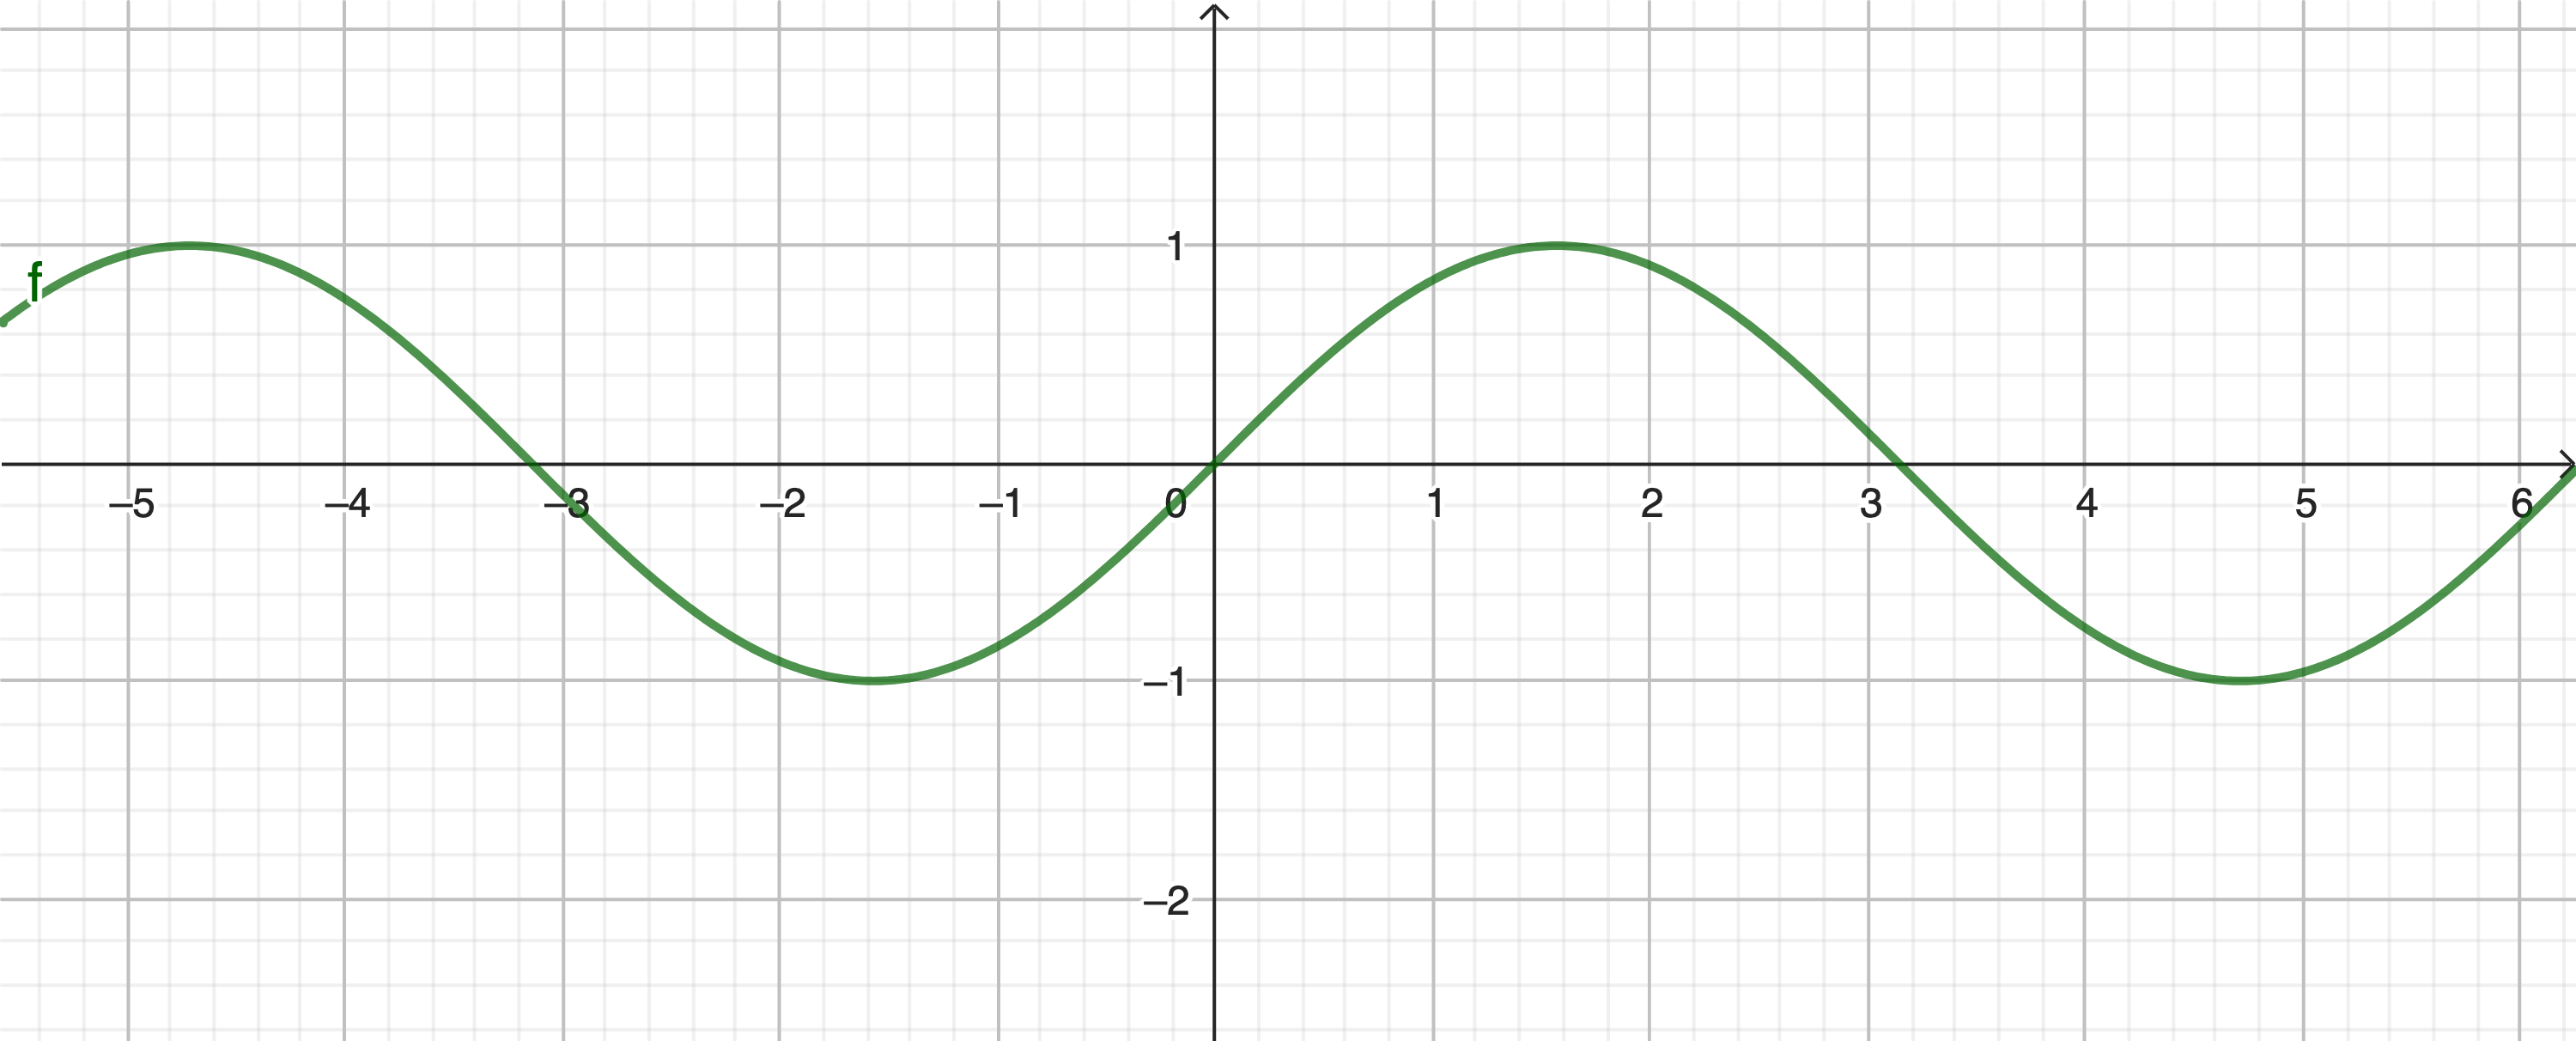
\includegraphics[width = 0.5 \textwidth]{media/IntroTaylor.png}
	\end{center}
	Ein Polynom ersten Grades ist eine lineare Funktion. Der Graph ist eine Gerade.

	Welche Gerade nähert sich um die Stelle $x_0=0$ am besten an den Graphen an?

	\vspace*{4cm}

	Approximation durch ein Polynom $T_2(x)$ 2. Grades:

	Ansatz: $T_2(x)=a_2x^2+a_1x+a_0$
	\vspace*{6cm}


\end{bsp}
\clearpage
\begin{LA}
	{Approximation der Sinusfunktion}{TaylorSinus}
	\begin{enumerate}
		\item 	Bestimmen Sie Näherungen der Funktion $f(x)=\sin(x)$ durch Polynome $T_3,T_4$ und $T_5$ vom Grad 3, 4 und 5 nach dem besprochenen Muster. Testen Sie jeweils die Genauigkeit an der Stelle $x=0.5$ (rad), indem Sie $\sin(0.5)$ mit $T_k (0.5)$ vergleichen.
		\item Können Sie die Polynome $T_6$ und $T_7$ angeben, ohne die ganze Rechnung erneut durchzuführen?
		\item Sei nun $f$ eine beliebige Funktion. 	Bestimmen Sie Polynomfunktionen $T_1,T_2$ und $T_3$ ersten, zweiten bzw. dritten Grades, die mit $f$ an der Stelle $x_0=0$ im Funktionswert und im Wert der 1., 2. und 3. Ableitung übereinstimmen.
		\item 	Wie lauten das Näherungspolynom $n$-ten Grades $T_n (x)$ für eine beliebige Funktion $f$?
	\end{enumerate}
\end{LA}

\clearpage



\clearpage
\section{Taylorpolynom und Taylorentwicklung}

\begin{figure}[h]
	\centering
	\begin{subfigure}[b]{0.3\textwidth}
		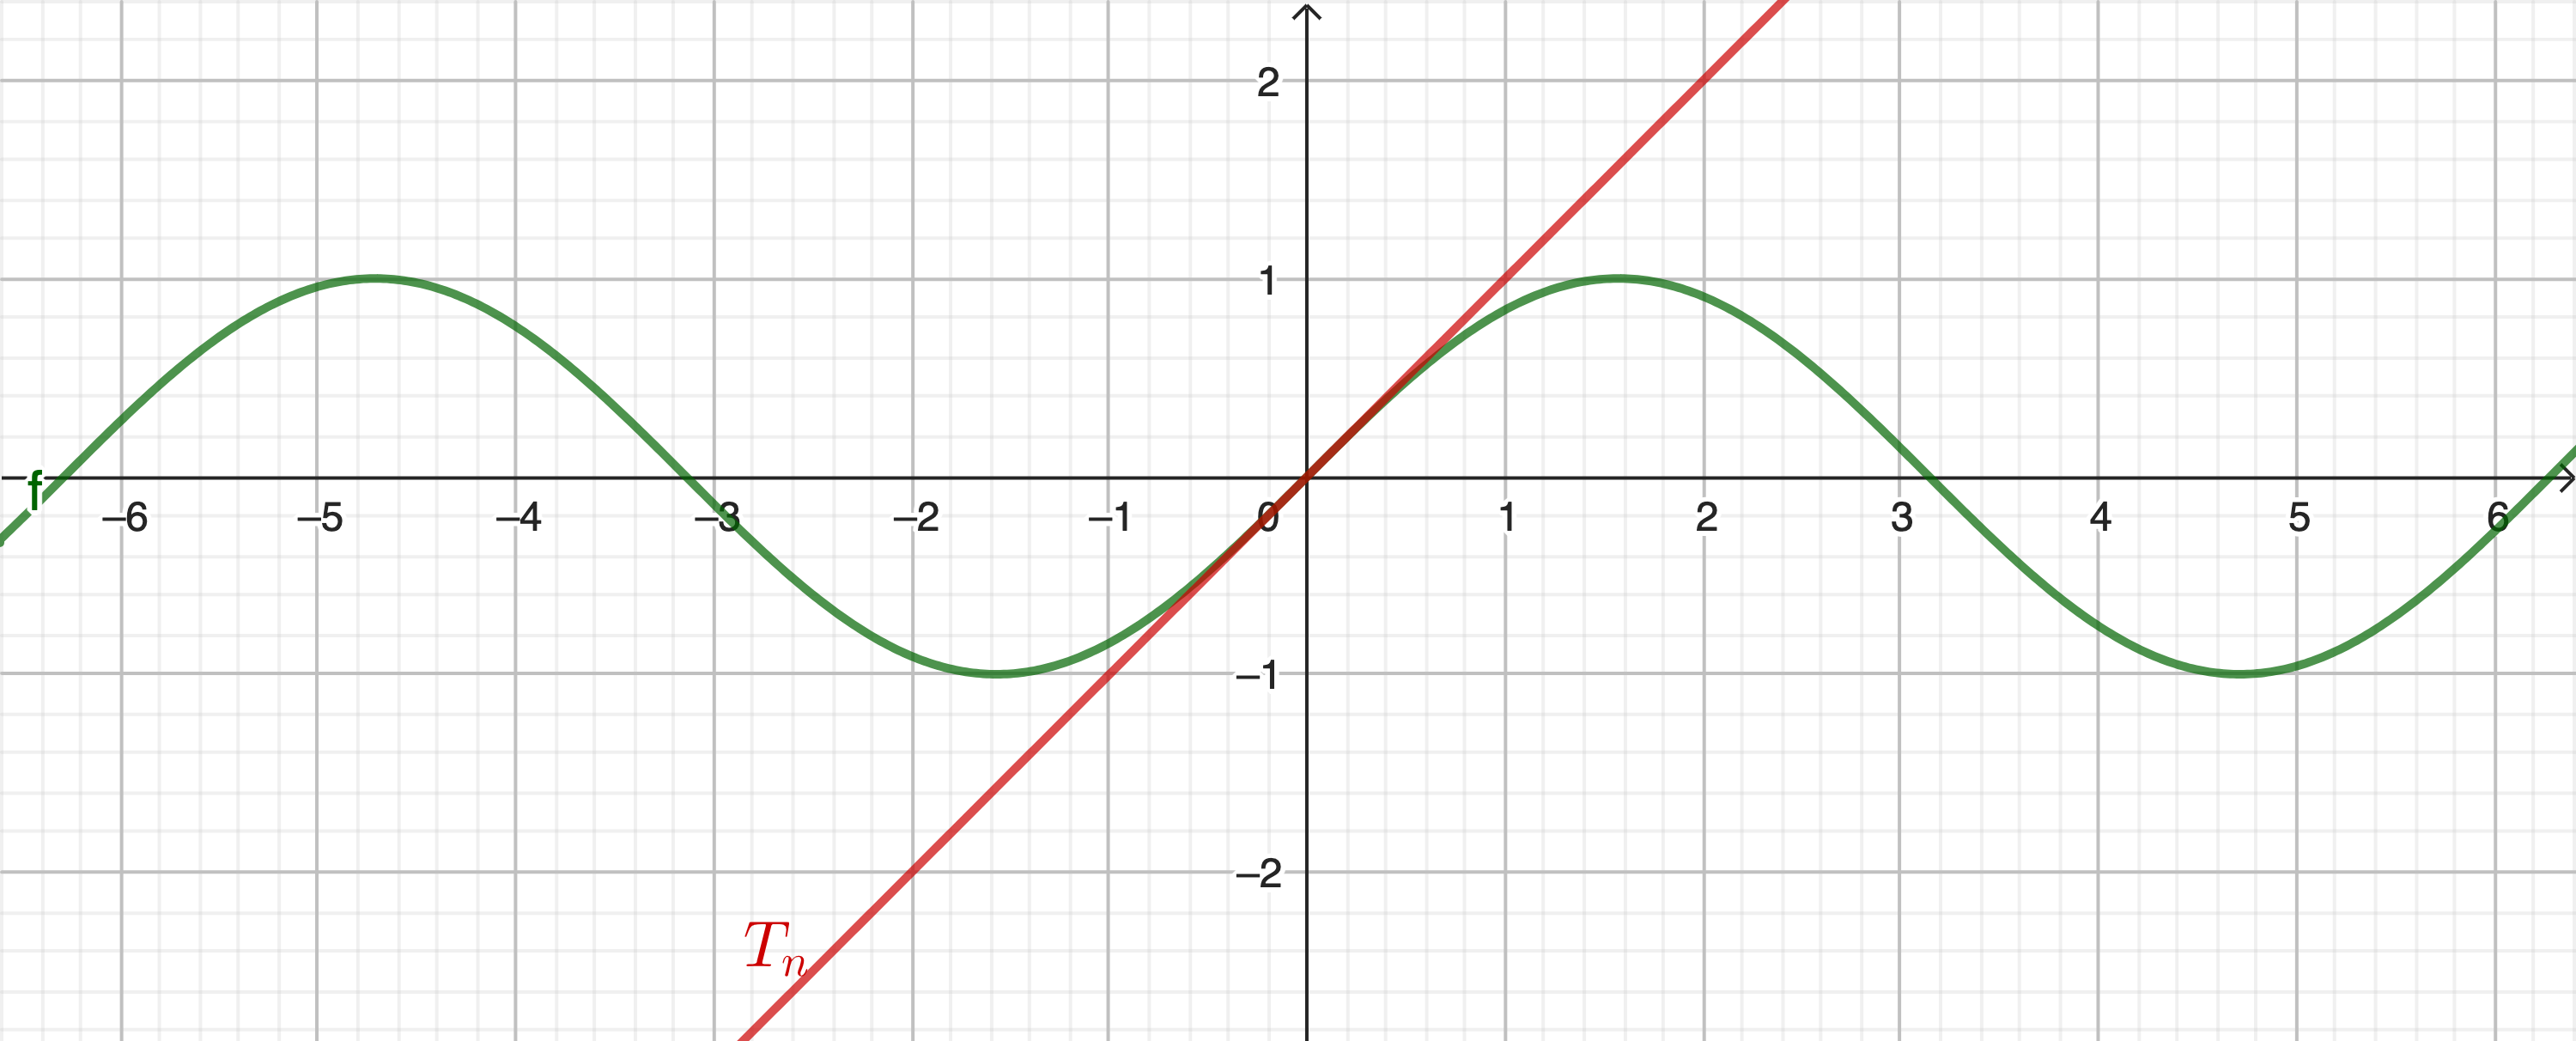
\includegraphics[width=\textwidth]{media/SinusT1.png}
		\caption*{Approximation durch ein Polynom von Grad 1}
	\end{subfigure}
	\begin{subfigure}[b]{0.3\textwidth}
		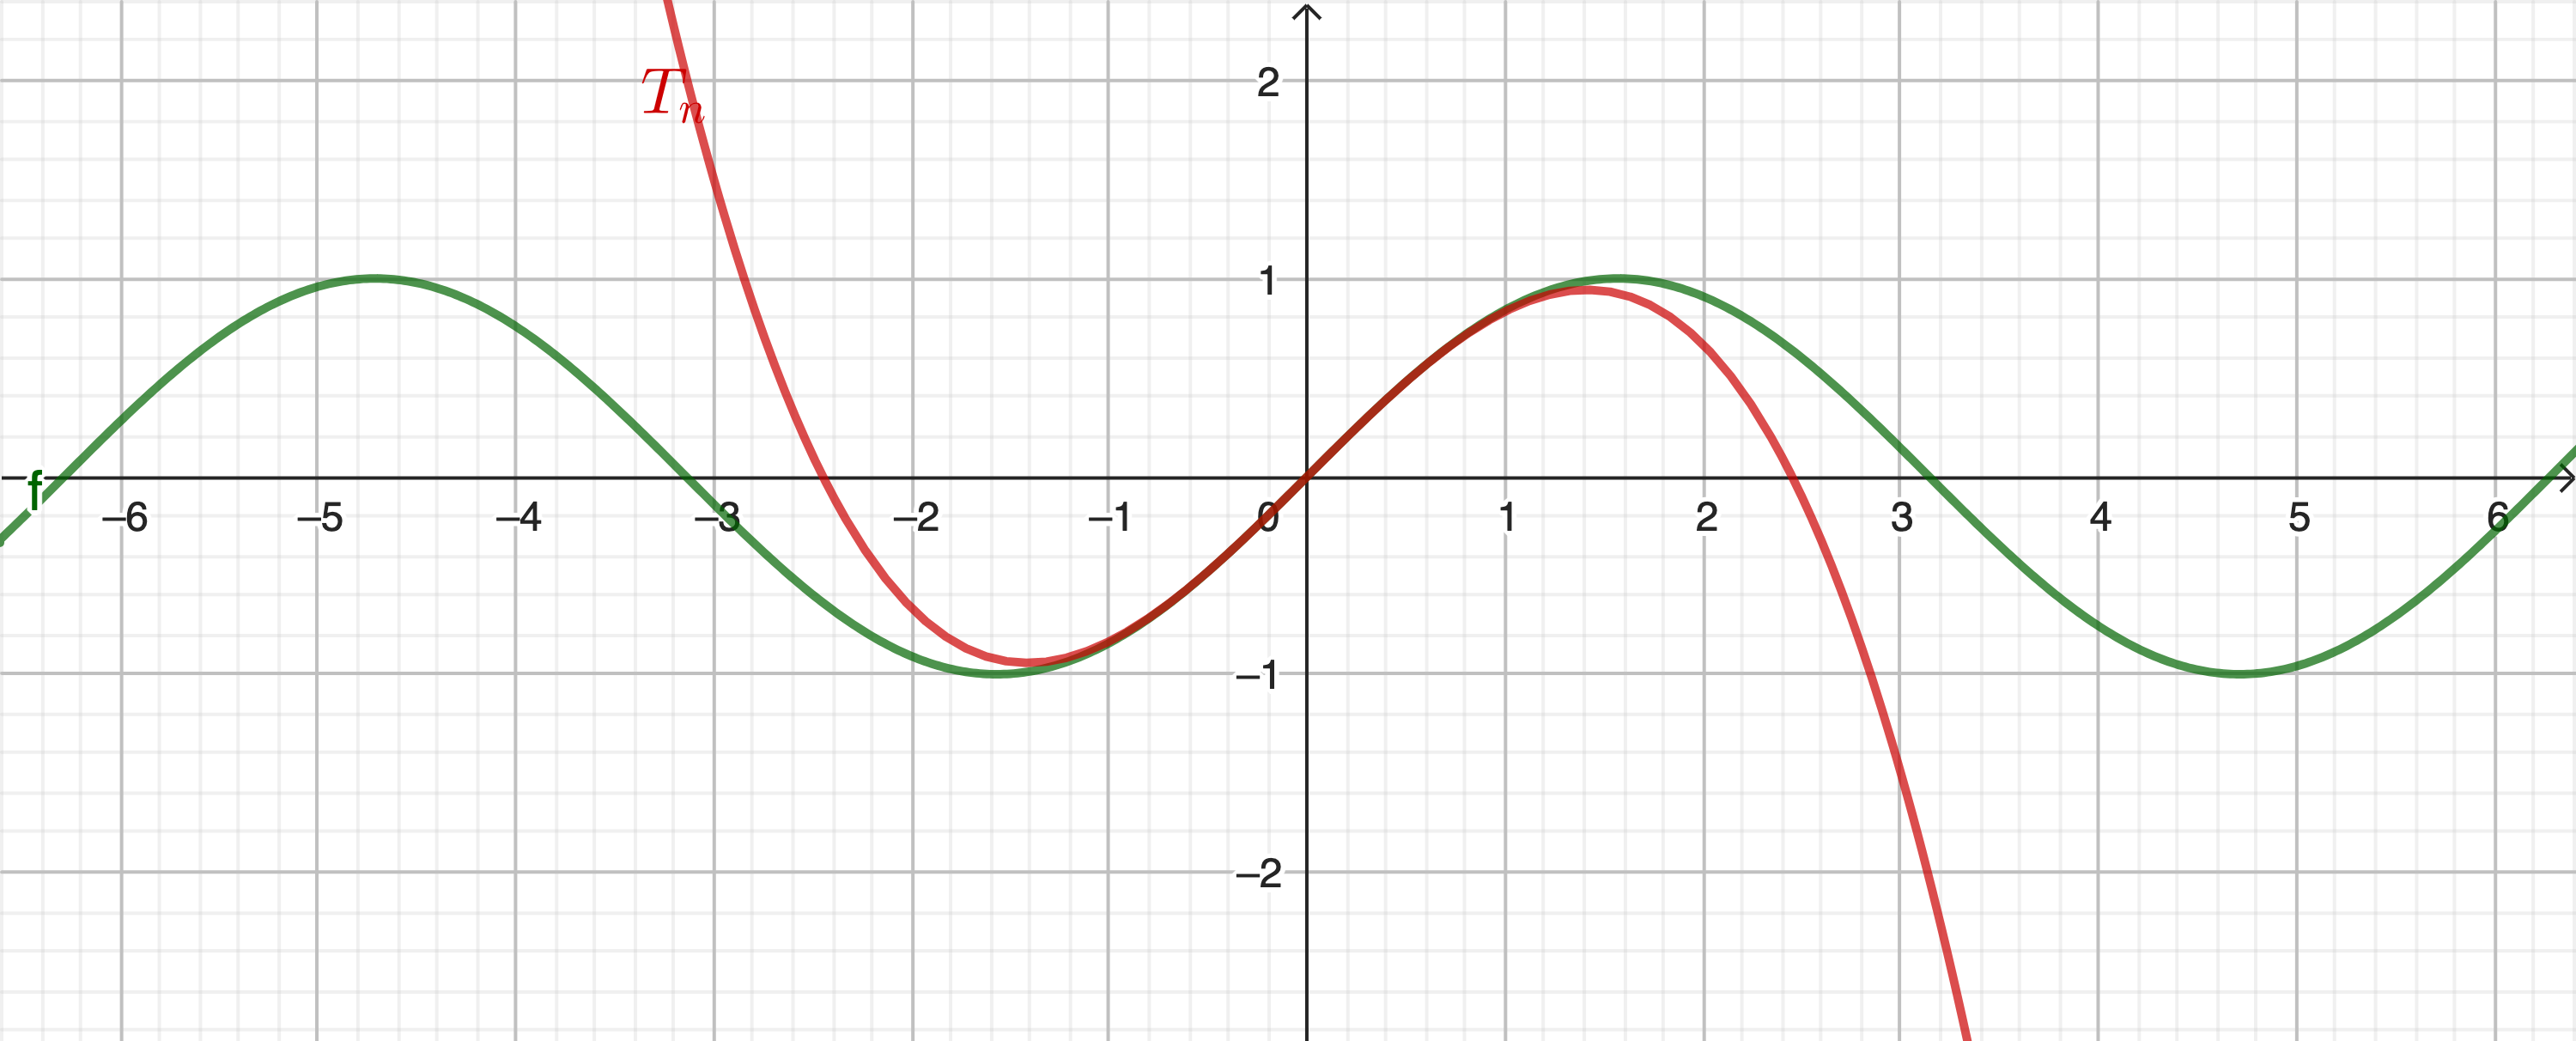
\includegraphics[width=\textwidth]{media/sinusT3.png}
		\caption*{Approximation durch ein Polynom von Grad 3}
	\end{subfigure}
	\begin{subfigure}[b]{0.3\textwidth}
		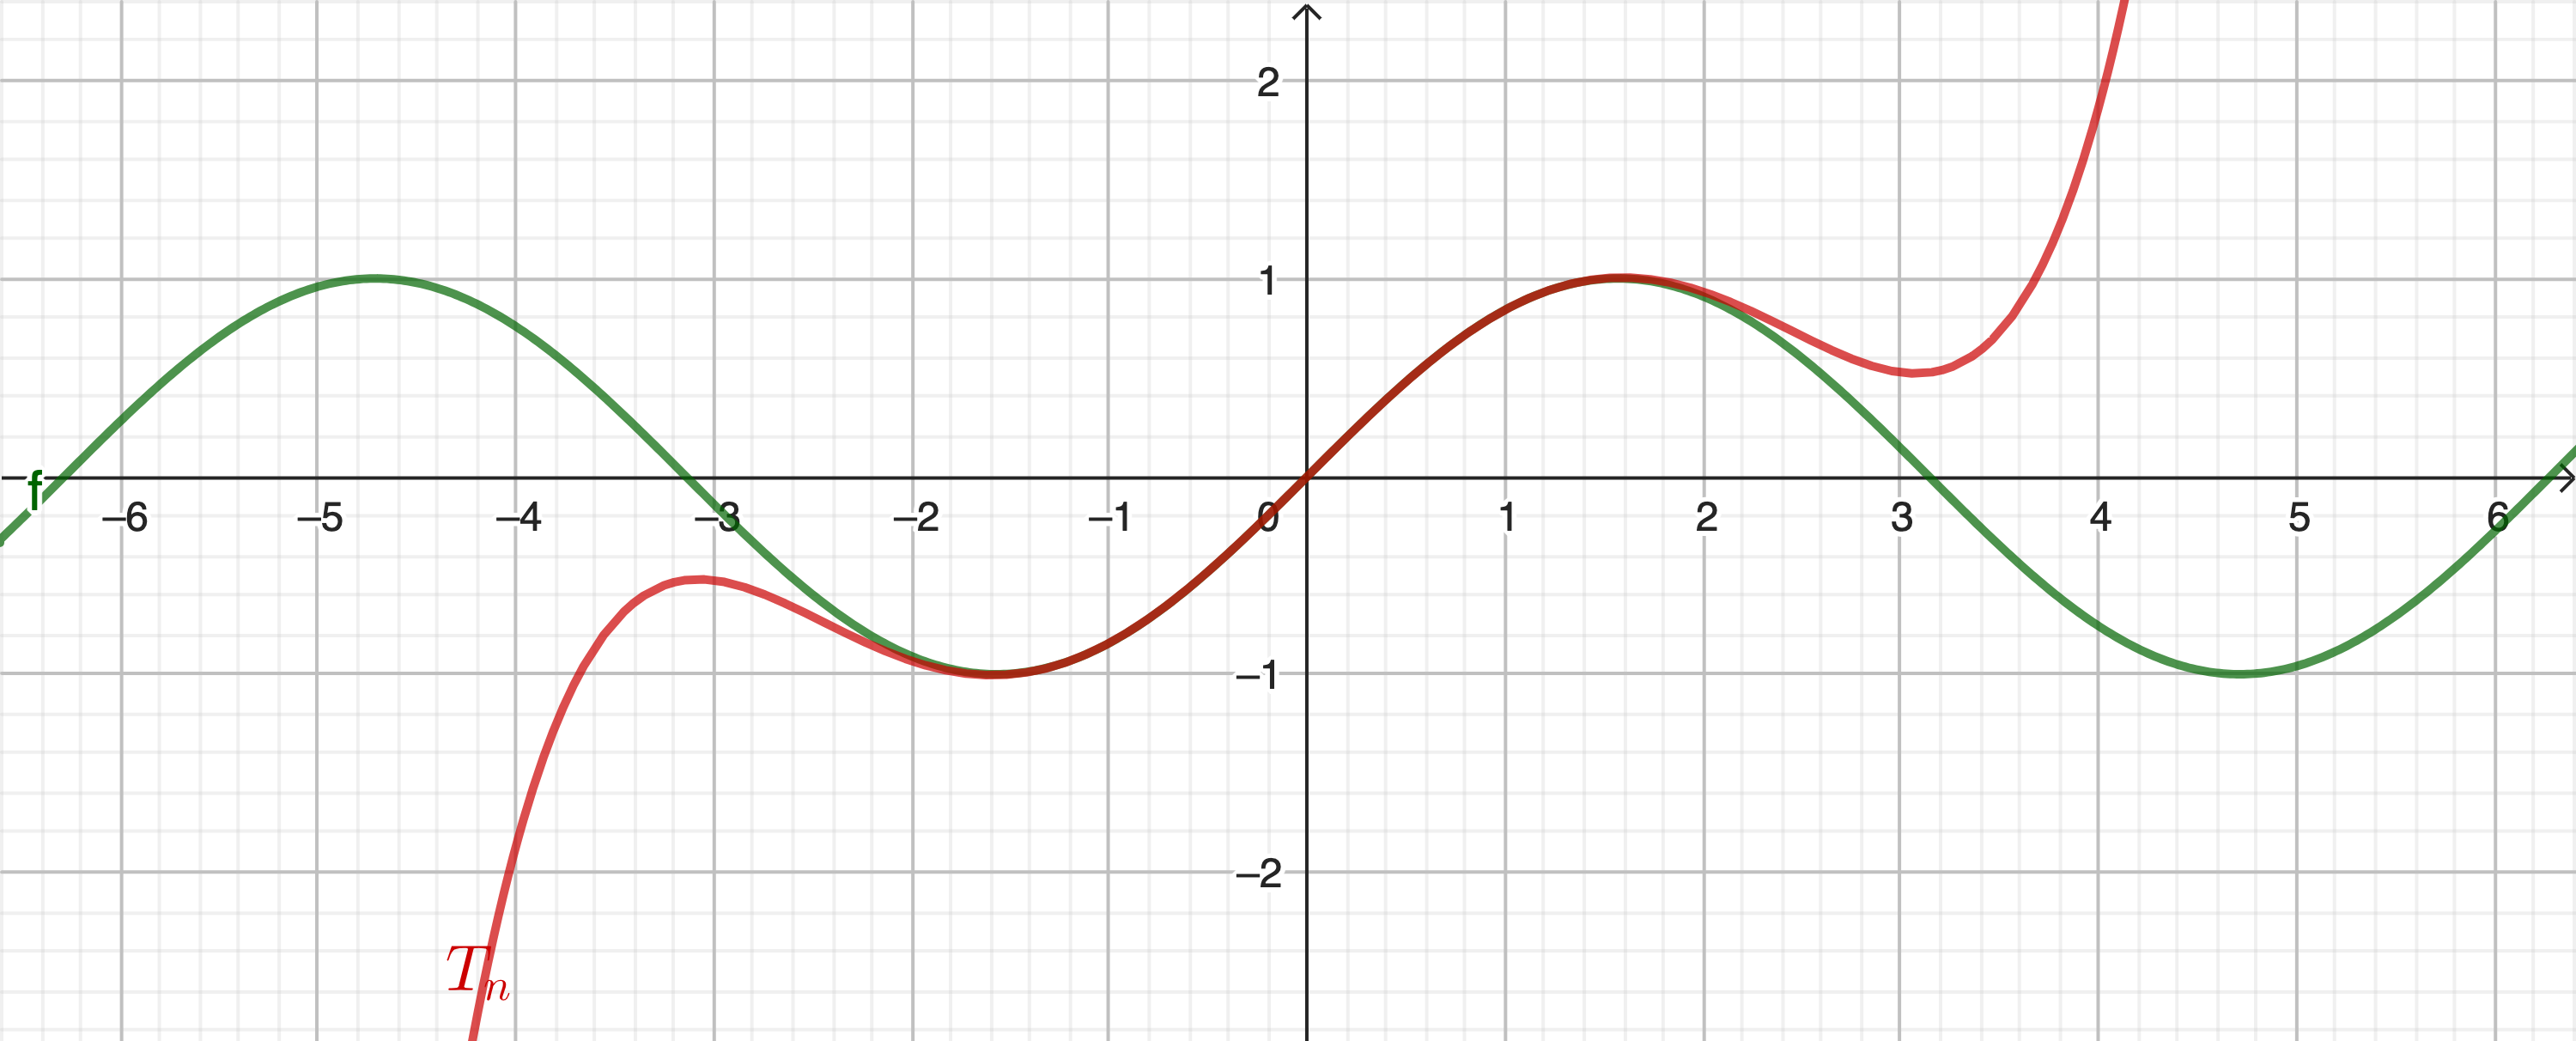
\includegraphics[width=\textwidth]{media/sinusT5.png}
		\caption*{Approximation durch ein Polynom von Grad 5}

	\end{subfigure}

\end{figure}
Die Bilder zeigen die Approximationen der Sinusfunktion durch Polynome 1., 3. und 5. Grades. Die Forderung nach weiterer Übereinstimmung in immer höheren Ableitungen führt zu immer besseren Näherungsfunktionen. Insbesondere wird der Bereich, in welchem die Taylorpolynome fast mit der Sinusfunktion übereinstimmen, immer grösser.

Wenn man diesen Prozess unendlich weiterdenkt, erhält man den folgenden Satz:
\begin{satz} {Taylorentwicklung der Sinusfunktion}{}
	$$ \sin(x) = x - \frac{1}{3!}x^3 + \frac{1}{5!}x^5 - \frac{1}{7!}x^7 + \frac{1}{9!}x^9 \pm \ldots = \sum_{k=0}^{\infty} (-1)^k \frac{x^{2k+1}}{(2k+1)!} $$
\end{satz}

Dieser Satz bildet den Schlüssel zur Berechnung von Sinuswerten unter Verwendung der vier Grundoperationen. Allerdings müsste man zur Ermittlung eines genauen Sinuswerts, unendlich viele Rechenoperationen durchführen. Deswegen verwendet man in der Praxis oft nur die ersten paar Summanden. Dabei argumentiert man wie folgt: Wenn $x$ nicht allzu gross ist, dann ist für grosse $n$  $x^n$ viel kleiner als $n!$ Also fallen die hinteren Terme der Summe  $\sum_{k=0}^{\infty} (-1)^k \frac{x^{2k+1}}{(2k+1)!}$ kaum ins Gewicht und es gilt:
$$\sin(x)\approx  x - \frac{1}{3!}x^3 + \frac{1}{5!}x^5 \qquad \text{, für $|x|$  klein} $$
Dabei gilt: Je kleiner $|x|$, desto weniger Summanden sind nötig, um eine bestimmte Genauigkeit zu erreichen und umgekehrt.

Eine solche Approximation der Sinusfunktion durch Polynome bildet die Grundidee, wie man mit dem Taschenrechner gute Näherungen für die Werte von $\sin(x)$ erzeugen kann. Allerdings verwendet der Taschenrechner in Wahrheit aus Speicher- und Laufzeitgründen eine andere, kompliziertere Methode, auf die wir hier nicht weiter eingehen werden.

Die Idee, wie wir die Sinusfunktion approximiert haben, lässt auch auf andere Funktionen anwenden:
\begin{definition}
	{Taylorpolynom}{}
	Sei $f$ eine Funktion, die an der Stelle $x_0=0$ $n$-mal differenzierbar ist. Dann nennt man
	\[
		T_n(x) = f(0) + \frac{f'(0)}{1!} \cdot x + \frac{f''(0)}{2!} \cdot x^2 + \frac{f'''(0)}{3!} \cdot x^3 + \ldots + \frac{f^{(n)}(0)}{n!} \cdot x^n = \sum_{k=0}^{n} \frac{f^{(k)}(0)}{k!} \cdot x^k
	\]
	das \emph{Taylorpolynom} $n$-ten Grades von $f$ um die Entwicklungsstelle $x_0=0$.
\end{definition}
Analog der unendliche Prozess:
\begin{definition}
	{Taylorreihe}{}
	Sei $f$ eine Funktion, die an der Stelle $x_0=0$ unendlich oft differenzierbar ist. Dann nennt man
	\[
		T(x) = f(0) + \frac{f'(0)}{1!} \cdot x + \frac{f''(0)}{2!} \cdot x^2 + \frac{f'''(0)}{3!} \cdot x^3 + \ldots = \sum_{k=0}^{\infty} \frac{f^{(k)}(0)}{k!} \cdot x^k
	\]
	die \emph{Taylorentwicklung oder die Taylorreihe} von $f$ um die Entwicklungsstelle $x_0=0$.
\end{definition}

Für jedes $x\in \R$ ist $T(x)$ eine unendliche Reihe. Jede dieser Reihen kann konvergieren oder auch nicht (siehe nächstes Kapitel).
\begin{bsp}
	{Die Taylorreihe der Sinusfunktion}{}

	Sei \( f(x) = \sin(x) \), dann gilt \[ f'(x) = \cos(x), \, f''(x) = -\sin(x) ,\, f^{(3)}(x) = -\cos(x) ,\,  f^{(4)}(x) = \sin(x) ,\, \ldots\]

	Daraus folgt wiederum, dass \[ f(0) = 0 ,\,  f'(0) = 1 ,\, f''(0) = 0 ,\,  f^{(3)}(0) = -1 ,\,  f^{(4)}(0) = 0 ,\, \ldots \]

	Damit lautet die Taylorreihe der Sinusfunktion:
	\[
		T(x) = 0 + \frac{1}{1!}x + \frac{0}{2!}x^2 - \frac{1}{3!}x^3 + \frac{0}{4!}x^4 + \ldots
		= x - \frac{x^3}{3!} + \frac{x^5}{5!} - \frac{x^7}{7!} \pm \ldots
		= \sum_{k=0}^{\infty} \frac{(-1)^k}{(2k+1)!}x^{2k+1}
	\]
\end{bsp}

Die Taylorpolynome liefern im Allgemeinen eine Approximation der Funktion in der Nähe von $x_0=0$. Durch geeignetes Verschieben kann man auch eine Näherungsfunktion an einer beliebigen anderen Stelle angeben:

\begin{definition}
	{Taylorpolynom und Taylorreihe an beliebiger Stelle}{}
	Sei \( f(x) \) eine Funktion, die an der Stelle \( x_0 \) unendlich oft differenzierbar ist. Dann nennt man

	\begin{align*}
		T_{n,x_0}(x) & = f(x_0) + \frac{f'(x_0)}{1!}(x-x_0) + \frac{f''(x_0)}{2!}(x-x_0)^2 + \ldots + \frac{f^{(n)}(x_0)}{n!}(x-x_0)^n \\
		             & = \sum_{k=0}^{n} \frac{f^{(k)}(x_0)}{k!}(x-x_0)^k
	\end{align*}

	Das Taylorpolynom \(n\)-ten Grades von \(f\) um die Entwicklungsstelle \(x_0\).

	Analog nennt man:

	\[
		T_{x_0}(x) = f(x_0) + \frac{f'(x_0)}{1!}(x-x_0) + \frac{f''(x_0)}{2!}(x-x_0)^2 + \ldots = \sum_{k=0}^{\infty} \frac{f^{(k)}(x_0)}{k!}(x-x_0)^k
	\]

	Die Taylorreihe von \(f\) um die Entwicklungsstelle \(x_0\).

\end{definition}

\begin{bsp}
	{Die Taylorreihe der Sinusfunktion um $x_0=\frac{\pi}{2}$}{}
	Sei \( f(x) = \sin(x) \). Dann gilt \( f\left(\frac{\pi}{2}\right) = 1 \), \( f'\left(\frac{\pi}{2}\right) = 0 \), \( f''\left(\frac{\pi}{2}\right) = -1 \), \( f'''\left(\frac{\pi}{2}\right) = 0 \), \( f^{(4)}\left(\frac{\pi}{2}\right) = 1 \), ...

	Daraus folgt
	\begin{align*}
		T_{\frac{\pi}{2}}(x) & = 1 + \frac{0}{1!}\left(x-\frac{\pi}{2}\right) + \frac{\left(-1\right)}{2!}\left(x-\frac{\pi}{2}\right)^2 + \frac{0}{3!}\left(x-\frac{\pi}{2}\right)^3 + \frac{1}{4!}\left(x-\frac{\pi}{2}\right)^4 + \ldots \\
		                     & = 1 - \frac{\left(x-\frac{\pi}{2}\right)^2}{2!} + \frac{\left(x-\frac{\pi}{2}\right)^4}{4!} - \frac{\left(x-\frac{\pi}{2}\right)^6}{6!} \pm \ldots                                                           \\
		                     & = \sum_{k=0}^{\infty} \frac{\left(-1\right)^k}{\left(2k\right)!}\left(x-\frac{\pi}{2}\right)^{2k}
	\end{align*}



\end{bsp}
\begin{ueb}
	{}{}

	\begin{enumerate}
		\item Bestimmen Sie die Taylorpolynome 3. Grades der folgenden Funktionen um die Entwicklungsstelle $x_0=0$. Geben Sie nach Möglichkeit auch die vollständige Taylorentwicklung mit einem Summenzeichen an:
		      \begin{enumerate}
			      \item $f(x) = \cos(x)$
			      \item $f(x)= e^x$
			      \item $f(x)= \frac{1}{1+x}=(1+x)^{-1}$
			      \item $f(x)= (x+1)^2$
			      \item $f(x)= 5x^5-7x^4+3x^3+2x+1$
		      \end{enumerate}
		\item Zeichnen Sie mit dem Computer die Graphen von $f(x)=e^x$ und von dessen Entwicklungen $T_1 (x),T_2 (x),T_3 (x)$. Verfolgen sie die wachsende Übereinstimmung.
		\item Stellen Sie die Funktion $f(x)=e^x$ als unendliche Taylorreihe dar und bestimmen Sie summandenweise die Ableitung der Reihe. Was fällt Ihnen auf?
		\item 	Betrachten Sie die Taylorreihe der Funktion $g(x)=\sin(x)$. Bestimmen Sie summandenweise die Ableitung der Reihe.
		\item Sei $v$ die Relativgeschwindigkeit zweier Inertialsysteme. Dann wird die Zeitdilatation in der SRT mit dem Lorentzfaktor berechnet:
		      \[
			      \gamma(v) = \frac{1}{\sqrt{1 - \left(\frac{v}{c}\right)^2}} = \left(1 - \frac{1}{c^2}\cdot v^2\right)^{-\frac{1}{2}}
		      \]

		      Da für Vorgänge im Alltag das Verhältnis \( \frac{v}{c} \) sehr klein ist, wird der Lorentzfaktor oft angenähert durch
		      \[
			      \gamma(v) \approx 1 + \frac{v^2}{2c^2}
		      \]

		      Zeigen Sie, dass diese Annäherung dem Taylorpolynom 2. Grades entspricht.
		      \pagebreak

		\item 	Bestimmen Sie die Taylorpolynome 3. Grades der Funktion $f$ an der Stelle $x_0$
		      \begin{enumerate}
			      \item $f(x) = \ln(x),\, x_0 = 1$
			      \item $f(x) = e^x,\, x_0 = e$
			      \item $f(x) = \cos(x),\, x_0 = \frac{\pi}{2}$
			      \item $f(x) = \sqrt{x},\, x_0 = 1$
		      \end{enumerate}
		\item 	Sei $T_{x_0}  (x)$ die Taylorentwicklung von $f$ um die Stelle $x_0$.

		      Berechnen Sie $T'(x_0 ),T'' (x_0 ),T'''(x_0 )$.
	\end{enumerate}
\end{ueb}
\clearpage

\emph{Lösungen}
\begin{enumerate}
	\item Entwicklungen
	      \begin{enumerate}
		      \item \[T_3(x) = 1-\frac{x^2}{2} , \quad T(x) = \sum_{k=0}^{\infty} \frac{(-1)^k}{(2k)!} x^{2k}\]
		      \item         \[T_3(x) = 1+x+\frac{x^2}{2!}+\frac{x^3}{3!}, \quad T(x) = \sum_{k=0}^{\infty} \frac{x^k}{k!}\]
		      \item         \[T_3(x) = 1-x+x^2-x^3, \quad T(x) = \sum_{k=0}^{\infty} (-x)^k\]
		      \item  $$T_3(x) = x^2+2x+1 = T(x) $$
		      \item         \[T_3(x) = 3x^3+2x+1, \quad T(x) = 5x^5-7x^4+3x^3+2x+1 \]
	      \end{enumerate}
	\item Grafik
	\item \[(e^x )'=(1+x+\frac{x^2}{2}+\frac{x^3}{6}+\frac{x^4}{24}+\ldots)'\]
	      \[=0+ 1+\frac{2x}{2}+\frac{3x^2}{6}+\frac{4x^3}{24}+\ldots\]
	      \[= 1+x+\frac{x^2}{2}+\frac{x^3}{6}+\ldots=e^x\]
	      Oder mit Summenformeln:
	      \[(e^x )'=\left(\sum_{k=0}^{\infty} \frac{x^k}{k!}\right)'\]
	      \[=\sum_{k=1}^{\infty} \frac{kx^{k-1}}{k!}=\sum_{k=1}^{\infty} \frac{x^{k-1}}{(k-1)!}=\sum_{k=0}^{\infty} \frac{x^k}{k!}=e^x\]
	\item \[(\sin(x) )'=(x-\frac{x^3}{6}+\frac{x^5}{120}-\frac{x^7}{5040}+\ldots)'\]
	      \[=1-\frac{3x^2}{6}+\frac{5x^4}{120}-\frac{7x^6}{5040}+\ldots\]
	      \[=1-\frac{x^2}{2}+\frac{x^4}{24}-\frac{x^6}{720}+\ldots=\cos(x)\]
	      Oder mit Summenformeln:
	      \[\left(\sum_{k=0}^{\infty} \frac{(-1)^k}{(2k+1)!} x^{2k+1}\right)'\]
	      \[=\sum_{k=0}^{\infty} \frac{(2k+1)(-1)^k}{(2k+1)!} x^{2k}=\sum_{k=0}^{\infty} \frac{(-1)^k}{(2k)!} x^{2k}=\cos(x)\]
	\item Einige Zwischenresultate:

	      $ \gamma'(v) = \frac{v}{c^2}\cdot \left(1-\frac{v^2}{c^2}\right)^{-\frac{3}{2}}  $ und $\gamma''(v) = \frac{1}{c^2}\cdot \left(1-\frac{v^2}{c^2}\right)^{-\frac{3}{2}} + \frac{3v^2}{c^4} \left(1-\frac{v^2}{c^2}\right)^{-\frac{5}{2}} $


	      % \[\gamma(v)\approx 1+\frac{v^2}{2c^2} \]
	\item Taylor an anderer Stelle
	      \begin{enumerate}
		      \item \[(x-1)-\frac{(x-1)^2}{2}+\frac{(x-1)^3}{3}\]
		      \item \[e^e+e^e (x-e)+\frac{e^e}{2} (x-e)^2+\frac{e^e}{3!} (x-e)^3\]
		      \item \[-(x-\frac{\pi}{2})+\frac{(x-\frac{\pi}{2})^3}{6}\]
		      \item
		            \[1+\frac{(x-1)}{2}-\frac{(x-1)^2}{8}+\frac{(x-1)^3}{16}\]

	      \end{enumerate}
	\item
	      \[T'(x_0)=f'(x_0), T''(x_0)=f''(x_0), T'''(x_0)=f'''(x_0), \ldots\]

\end{enumerate}

\begin{satz}
	{Diese Taylorreihen sollten Sie auswendig lernen}{}

	\begin{align*}
		\sin(x) & = x - \frac{x^3}{3!} + \frac{x^5}{5!} - \frac{x^7}{7!} \pm \ldots = \sum_{k=0}^{\infty} \frac{(-1)^k}{(2k+1)!} x^{2k+1} \\
		\cos(x) & = 1 - \frac{x^2}{2!} + \frac{x^4}{4!} - \frac{x^6}{6!} \pm \ldots = \sum_{k=0}^{\infty} \frac{(-1)^k}{(2k)!} x^{2k}     \\
		e^x     & = 1 + \frac{x}{1!} + \frac{x^2}{2!} + \frac{x^3}{3!} + \ldots = \sum_{k=0}^{\infty} \frac{x^k}{k!}
	\end{align*}

\end{satz}
















\clearpage

%\input{E-konvergenz-Taylor.tex}
\section{Konvergenz von Taylorreihen}
\subsection{Einführung}

In diesem Kapitel werden wir eine Formel für die Abweichung der Taylorentwicklung von der tatsächlichen Funktion angeben. Ausserdem werden wir untersuchen, unter welchen Bedingungen die Taylorentwicklung konvergiert.

\begin{LA}
	{}{}
	Verwenden Sie für diese Aufgabe \href{https://www.geogebra.org}{geogebra}.
	\begin{enumerate}
		\item Zeichnen Sie den Graphen der Funktion $f(x)=\ln(x+1)$. (Eingabe f(x)=ln(x+1))
		\item Erzeugen Sie in Geogebra das Taylorpolynom $n$-ten Grades an der Entwicklungsstelle $x_0  =0$ (Eingabe TaylorReihe(f,0,n))\\
		      Hinweis: Durch den Befehl wird ein Schieberegler für $n$ erstellt, mit dem Sie den Grad des Taylorpolynoms verändern können.
		\item Untersuchen Sie das Verhalten der Taylorapproximation für verschiedene Werte von $n$ im Intervall $n=1$ bis $n=15$. Was stellen Sie fest?\\
		      Hinweis: In den Einstellungen des Schiebereglers können Sie den Minimal- und Maximalwert sowie die Schrittweite anpassen.
		      % \item 	Berechnen Sie die Differenz zwischen der Funktion $f$ und der Taylorentwicklung an den Stellen
		      %       \begin{enumerate}
		      % 	      \item $x=0.5$
		      % 	      \item $x=1$
		      % 	      \item $x=2$
		      %       \end{enumerate}
		\item 	Untersuchen Sie die Gleichung der unendlichen Taylorentwicklung von $f$ und argumentieren Sie, wieso die Reihe $T(2)$ divergiert.


	\end{enumerate}

\end{LA}
\clearpage
Die Taylorentwicklung einer Funktion $f$ ist in der Regel eine unendliche Summe, auch Reihe genannt. Solche Reihen können konvergieren oder auch nicht. Betrachten Sie dazu die folgenden Beispiele.
\begin{bsp}
	{Drei Beispiele für Taylorentwicklungen}{}
	\begin{enumerate}
		\item Die Taylorentwicklung von \(f(x) = \sin(x)\) lautet
		      \[T(x) = x - \frac{1}{3!}x^3 + \frac{1}{5!}x^5 - \frac{1}{7!}x^7 + \frac{1}{9!}x^9 \pm \ldots = \sum_{k=0}^{\infty} \frac{(-1)^k}{(2k+1)!} x^{2k+1}\]

		      Diese Reihe konvergiert für jedes \(x \in \mathbb{R}\) gegen \(\sin(x)\).
		\item Die Taylorentwicklung der Funktion \( f(x) = \begin{cases} e^{-\frac{1}{x^2}}, & \text{falls } x > 0 \\ 0, & \text{falls } x \leq 0 \end{cases} \) lautet
		      \[ T(x) = 0. \]

		      Offensichtlich konvergiert \( T(x) \) für jedes \( x \in \mathbb{R} \). Der Grenzwert 0 stimmt aber für alle \( x > 0 \) nicht mit dem Funktionswert überein.
		\item Die Taylorentwicklung von \( f(x) = \ln(1+x) \) ist
		      \[ T(x) = x - \frac{x^2}{2} + \frac{x^3}{3} - \frac{x^4}{4} \pm \ldots = \sum_{k=1}^{\infty} \frac{(-1)^{k+1}}{k} x^k \]

		      Wenn \( |x| > 1 \) ist, erhält man eine divergente Reihe. Für \( |x| < 1 \) hingegen konvergiert die Reihe gegen \( \ln(1+x) \).

	\end{enumerate}
\end{bsp}
Zusammengefasst erhalten wir folgenden Satz:
\begin{satz}
	{Konvergenz von Taylorreihen}{}
	Sei $T(x)$ die Taylorentwicklung einer Funktion $f$. Dann gibt es für jedes Argument $x$ drei Möglichkeiten:
	\begin{enumerate}
		\item Die Reihe $T(x)$ konvergiert und der Grenzwert ist $f(x)$
		\item         Die Reihe $T(x)$ konvergiert und der Grenzwert ist nicht $f(x)$
		\item
		      Die Reihe $T(x)$ divergiert
	\end{enumerate}

\end{satz}
\emph{Bemerkung}: Für die meisten Funktionen, die Sie kennen, gilt der erste Fall.

Will man eine Funktion durch ihre Taylorreihe darstellen, muss man also im Grunde zuerst beweisen, dass letztere wirklich konvergiert und dass der Grenzwert mit dem Funktionswert übereinstimmt.
Die Idee beim Beweis der Konvergenz einer Taylorreihe ist die, dass man die Abweichung der Taylorentwicklung $n$-ten Grades von dem tatsächlichen Funktionswert angibt, und anschliessend zeigt, dass diese Abweichung für wachsende $n$ gegen Null strebt.

\begin{definition}
	{Das $n$-te Restglied}{}
	Sei $T_n$ das Taylorpolynom $n$-ten Grades der Funktion $f$. Dann nennt man die Funktion
	$$R_n (x)=f(x)-T_n (x)$$
	das $n$-te Restglied der Taylorentwicklung.

\end{definition}
In anderen Worten: Das Restglied ist der Fehler, den man macht, wenn man die Funktion durch das Taylorpolynom $n$-ten Grades approximiert. Die folgenden vier Bilder zeigen die Sinusfunktion (blau), deren Taylorpolynom vom Grad $n=1, 3, 5, 7$ (orange), den Fehler $R_n(4)$ an der Stelle $x=4$ (rote Strecke) und der Verlauf der Funktion $y=R_n(x)$ (grün).

\begin{figure}[h!]
	\centering
	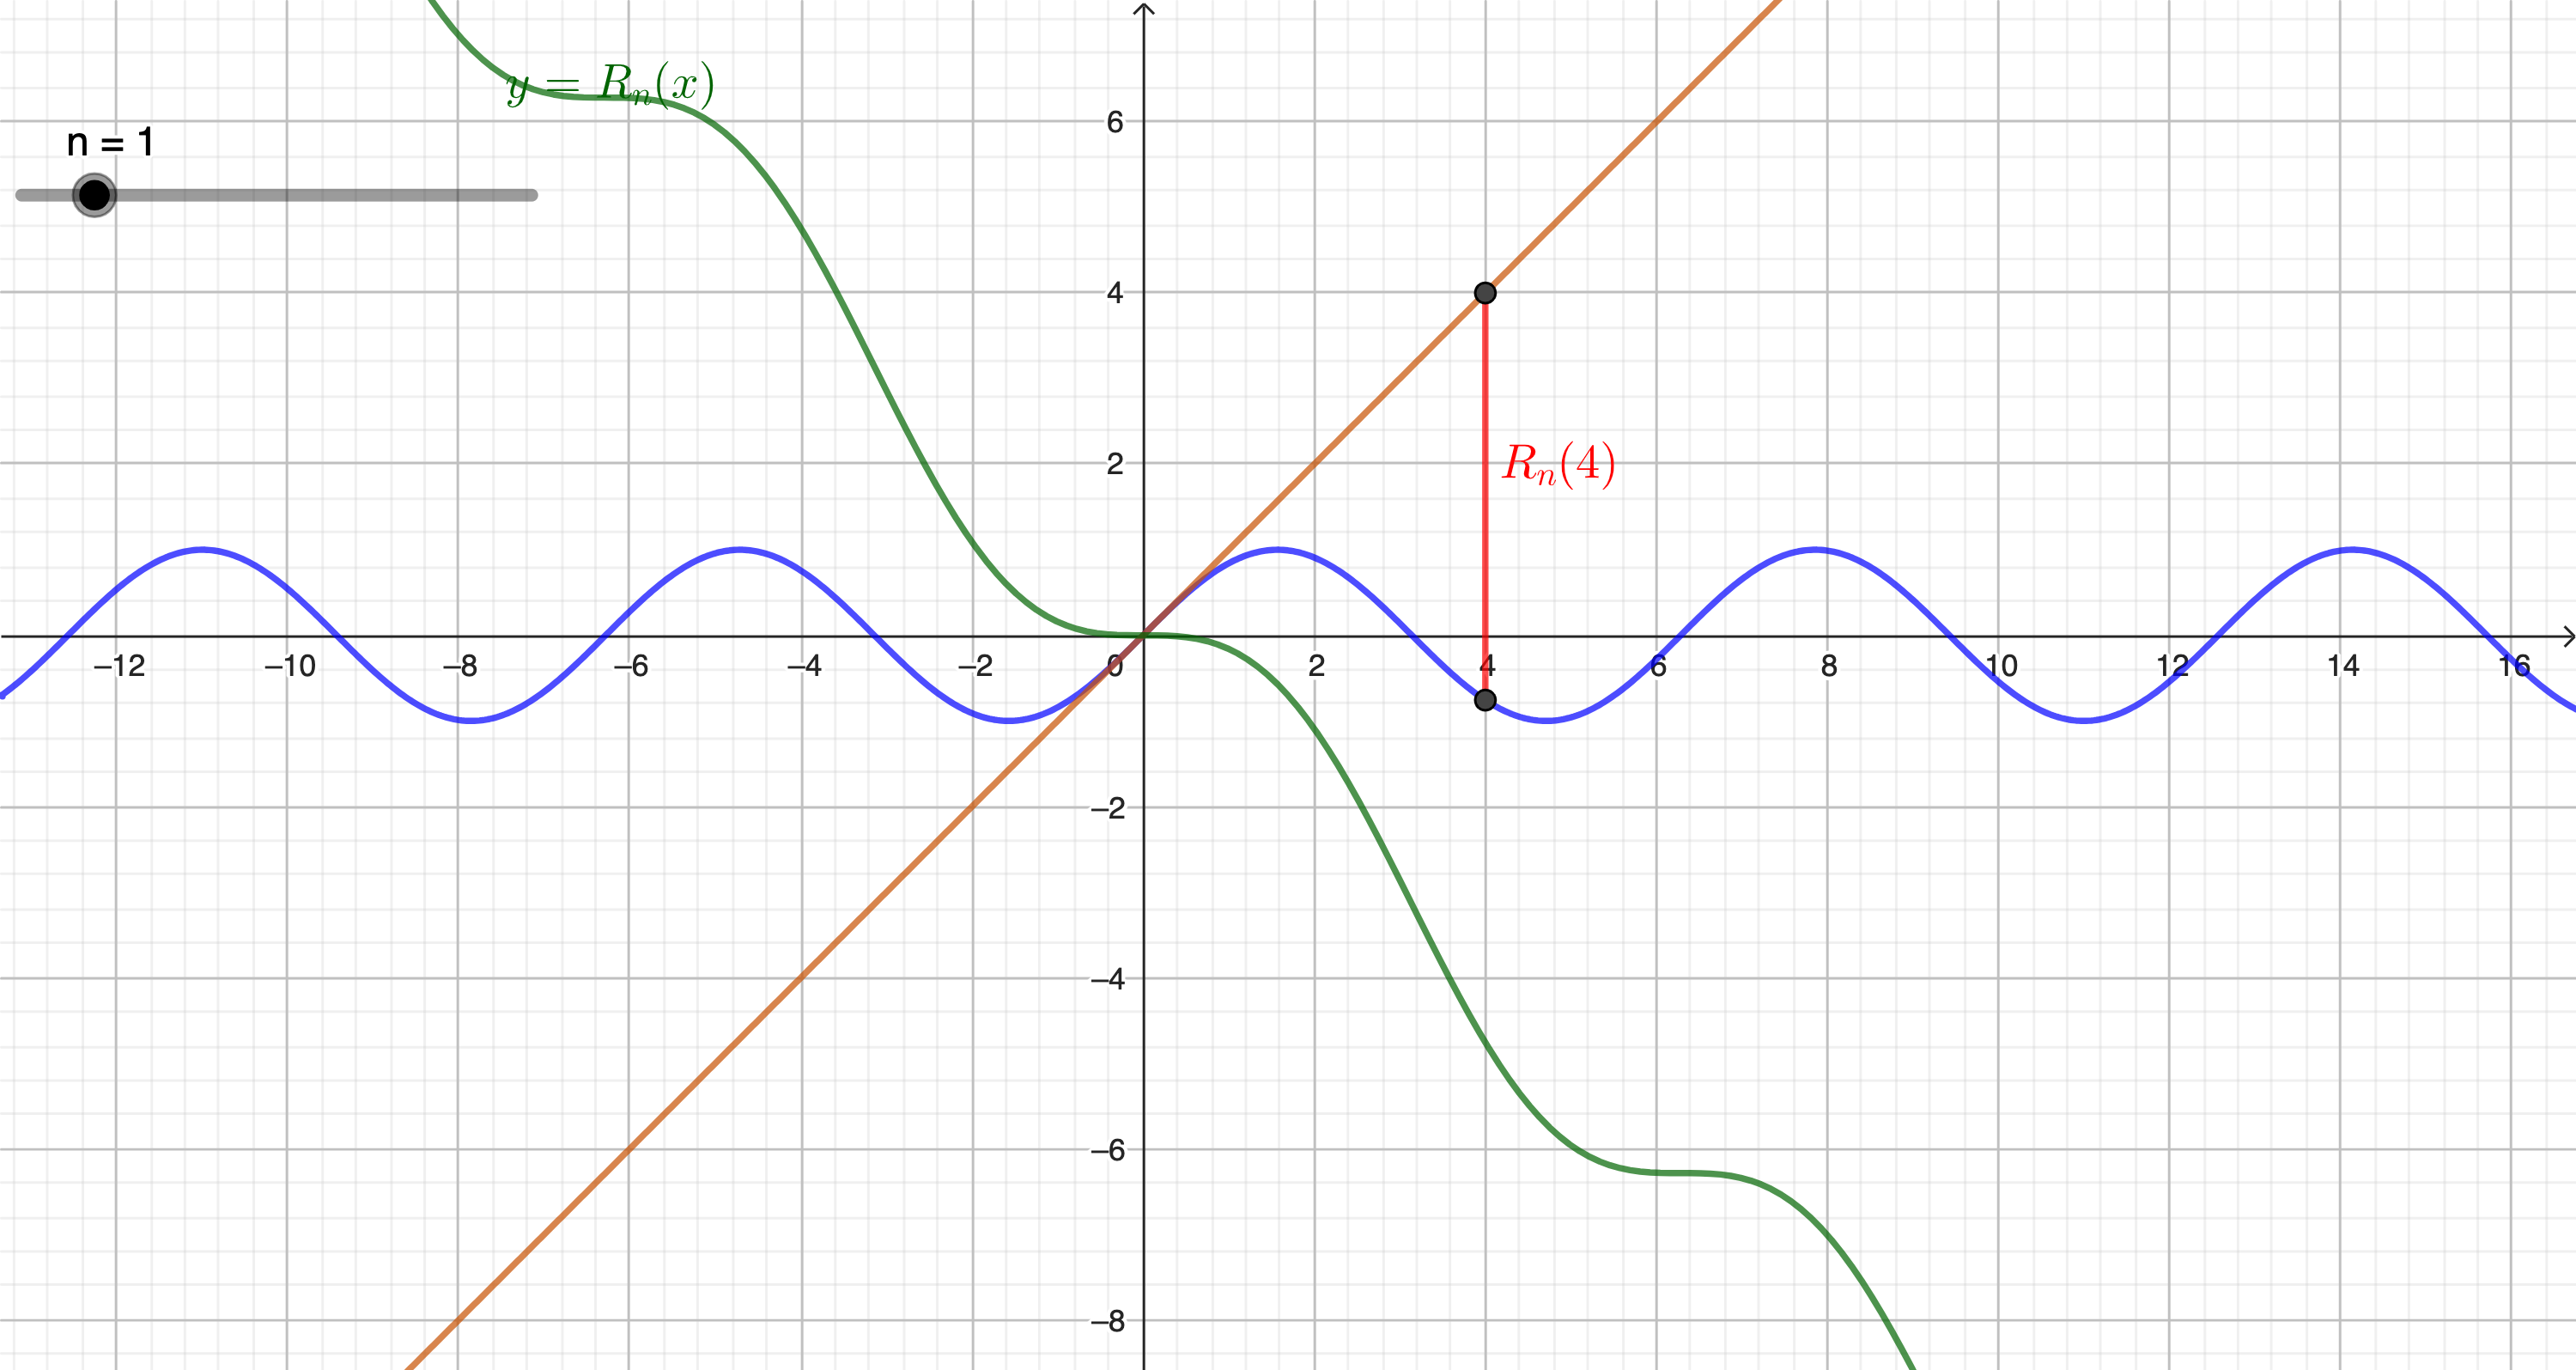
\includegraphics[width=0.45\textwidth]{media/restglied1.png}
	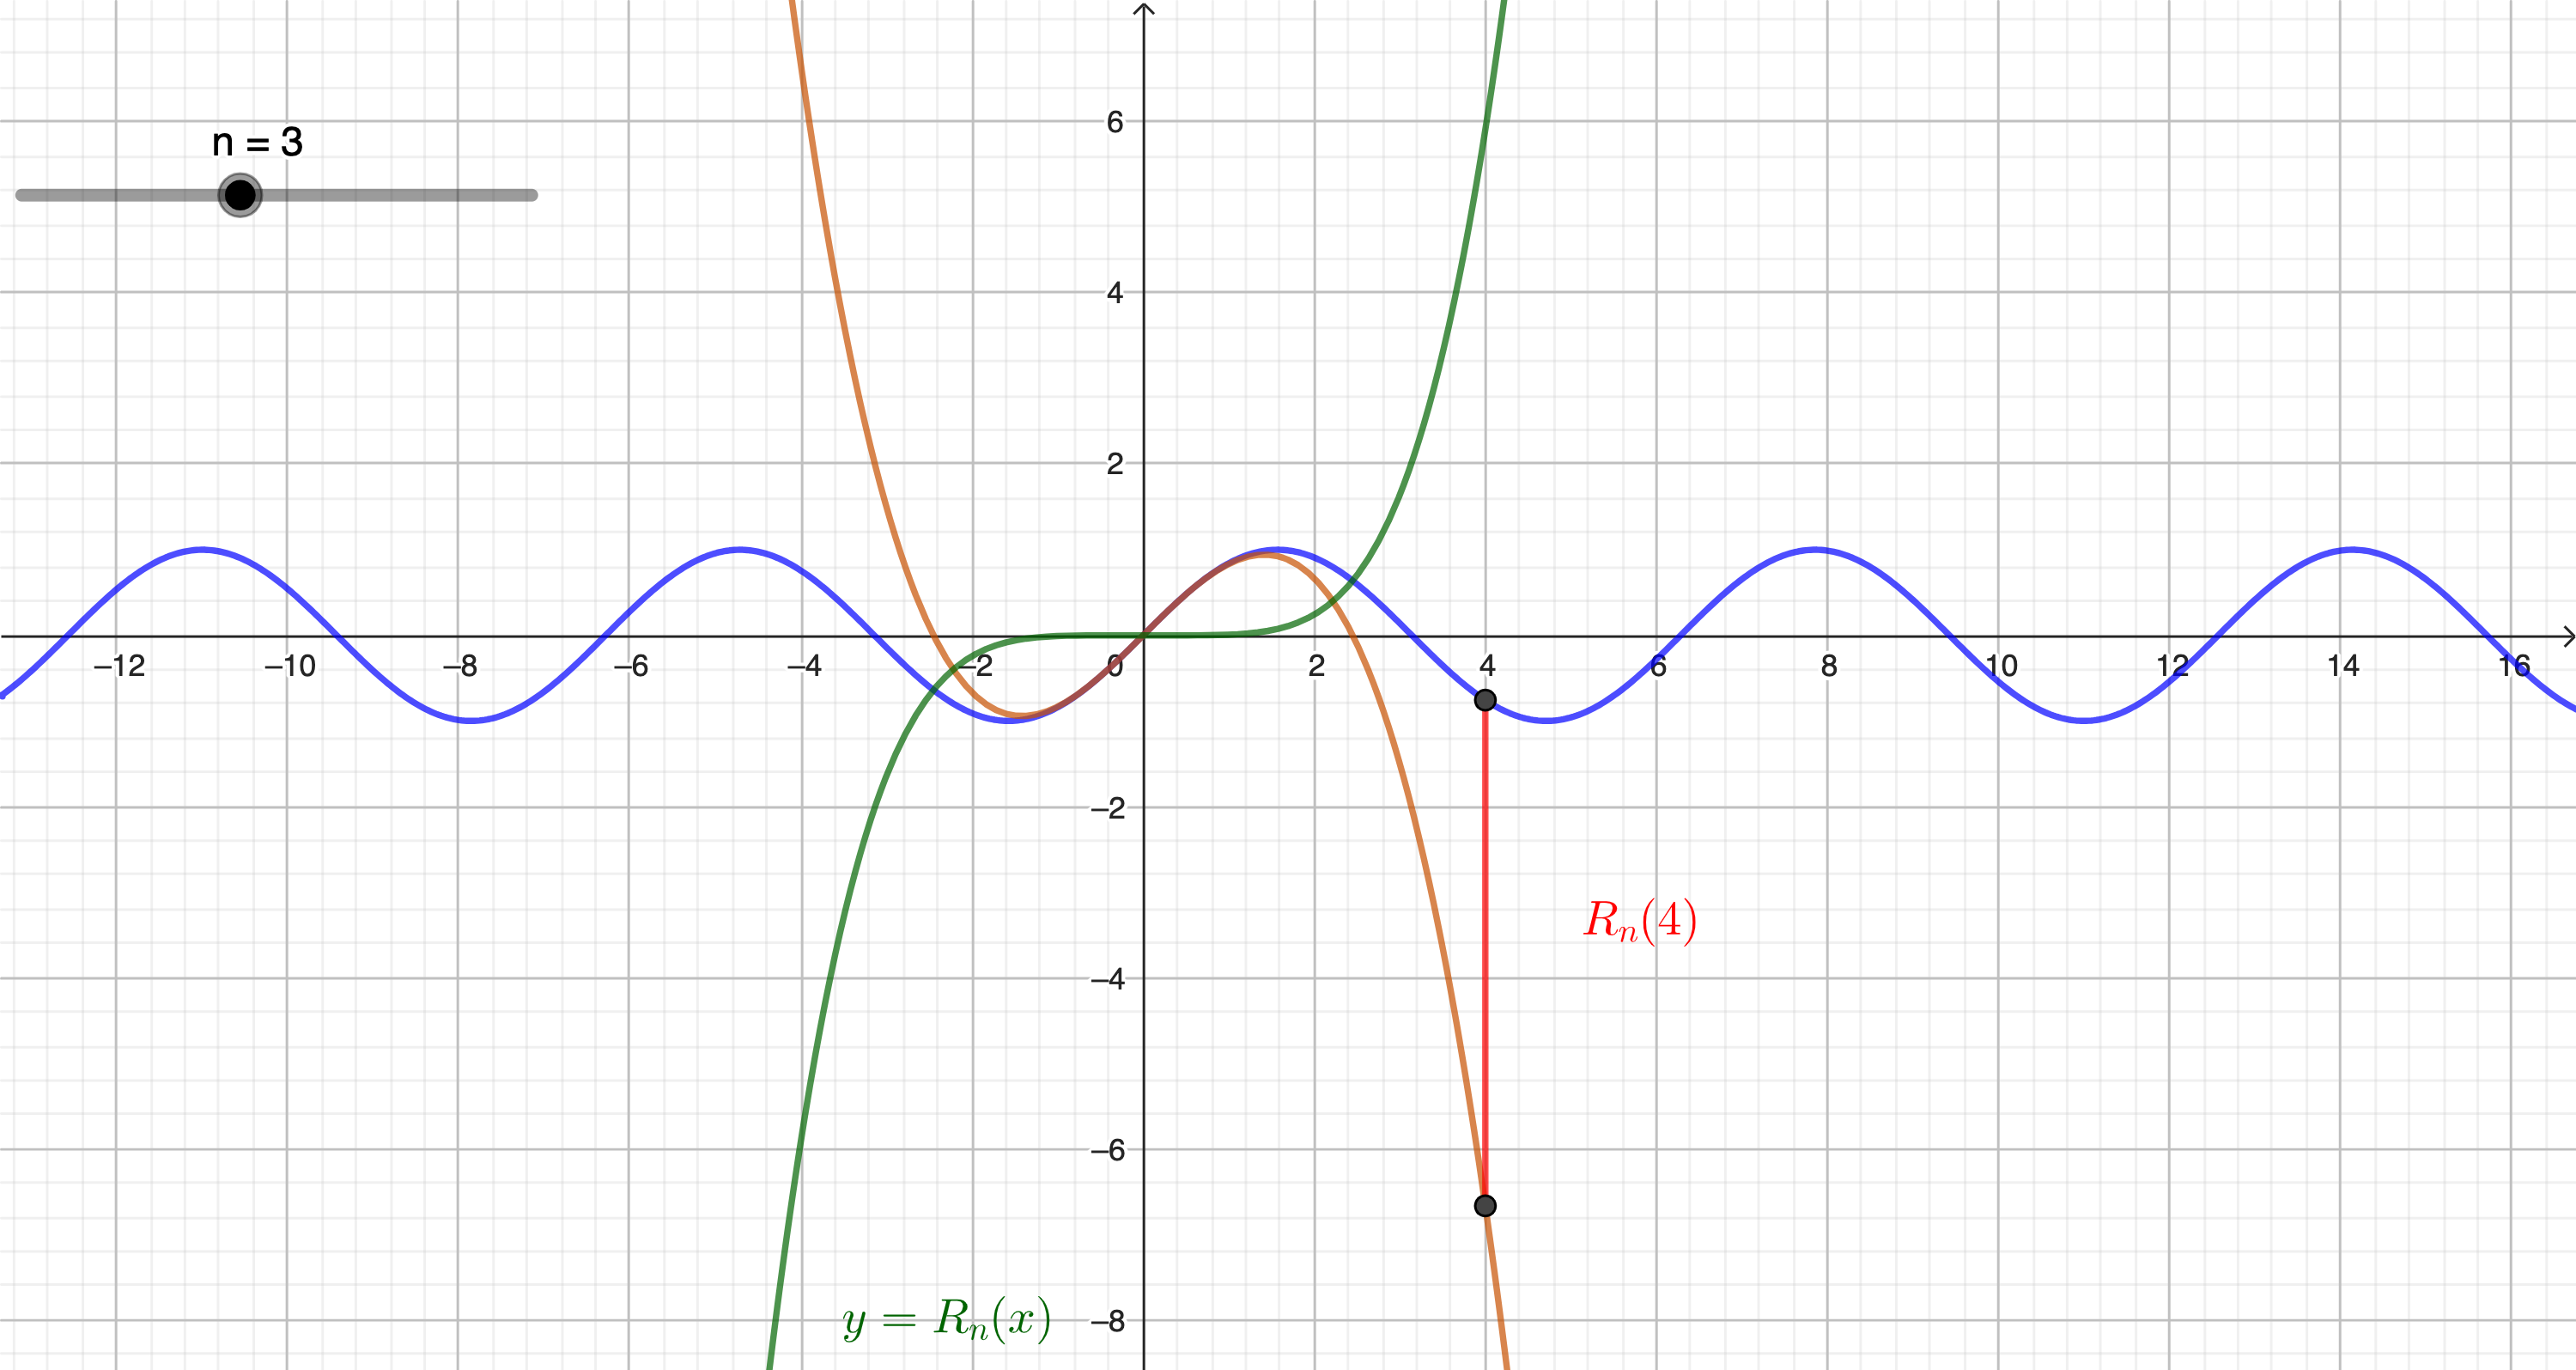
\includegraphics[width=0.45\textwidth]{media/restglied3.png}

	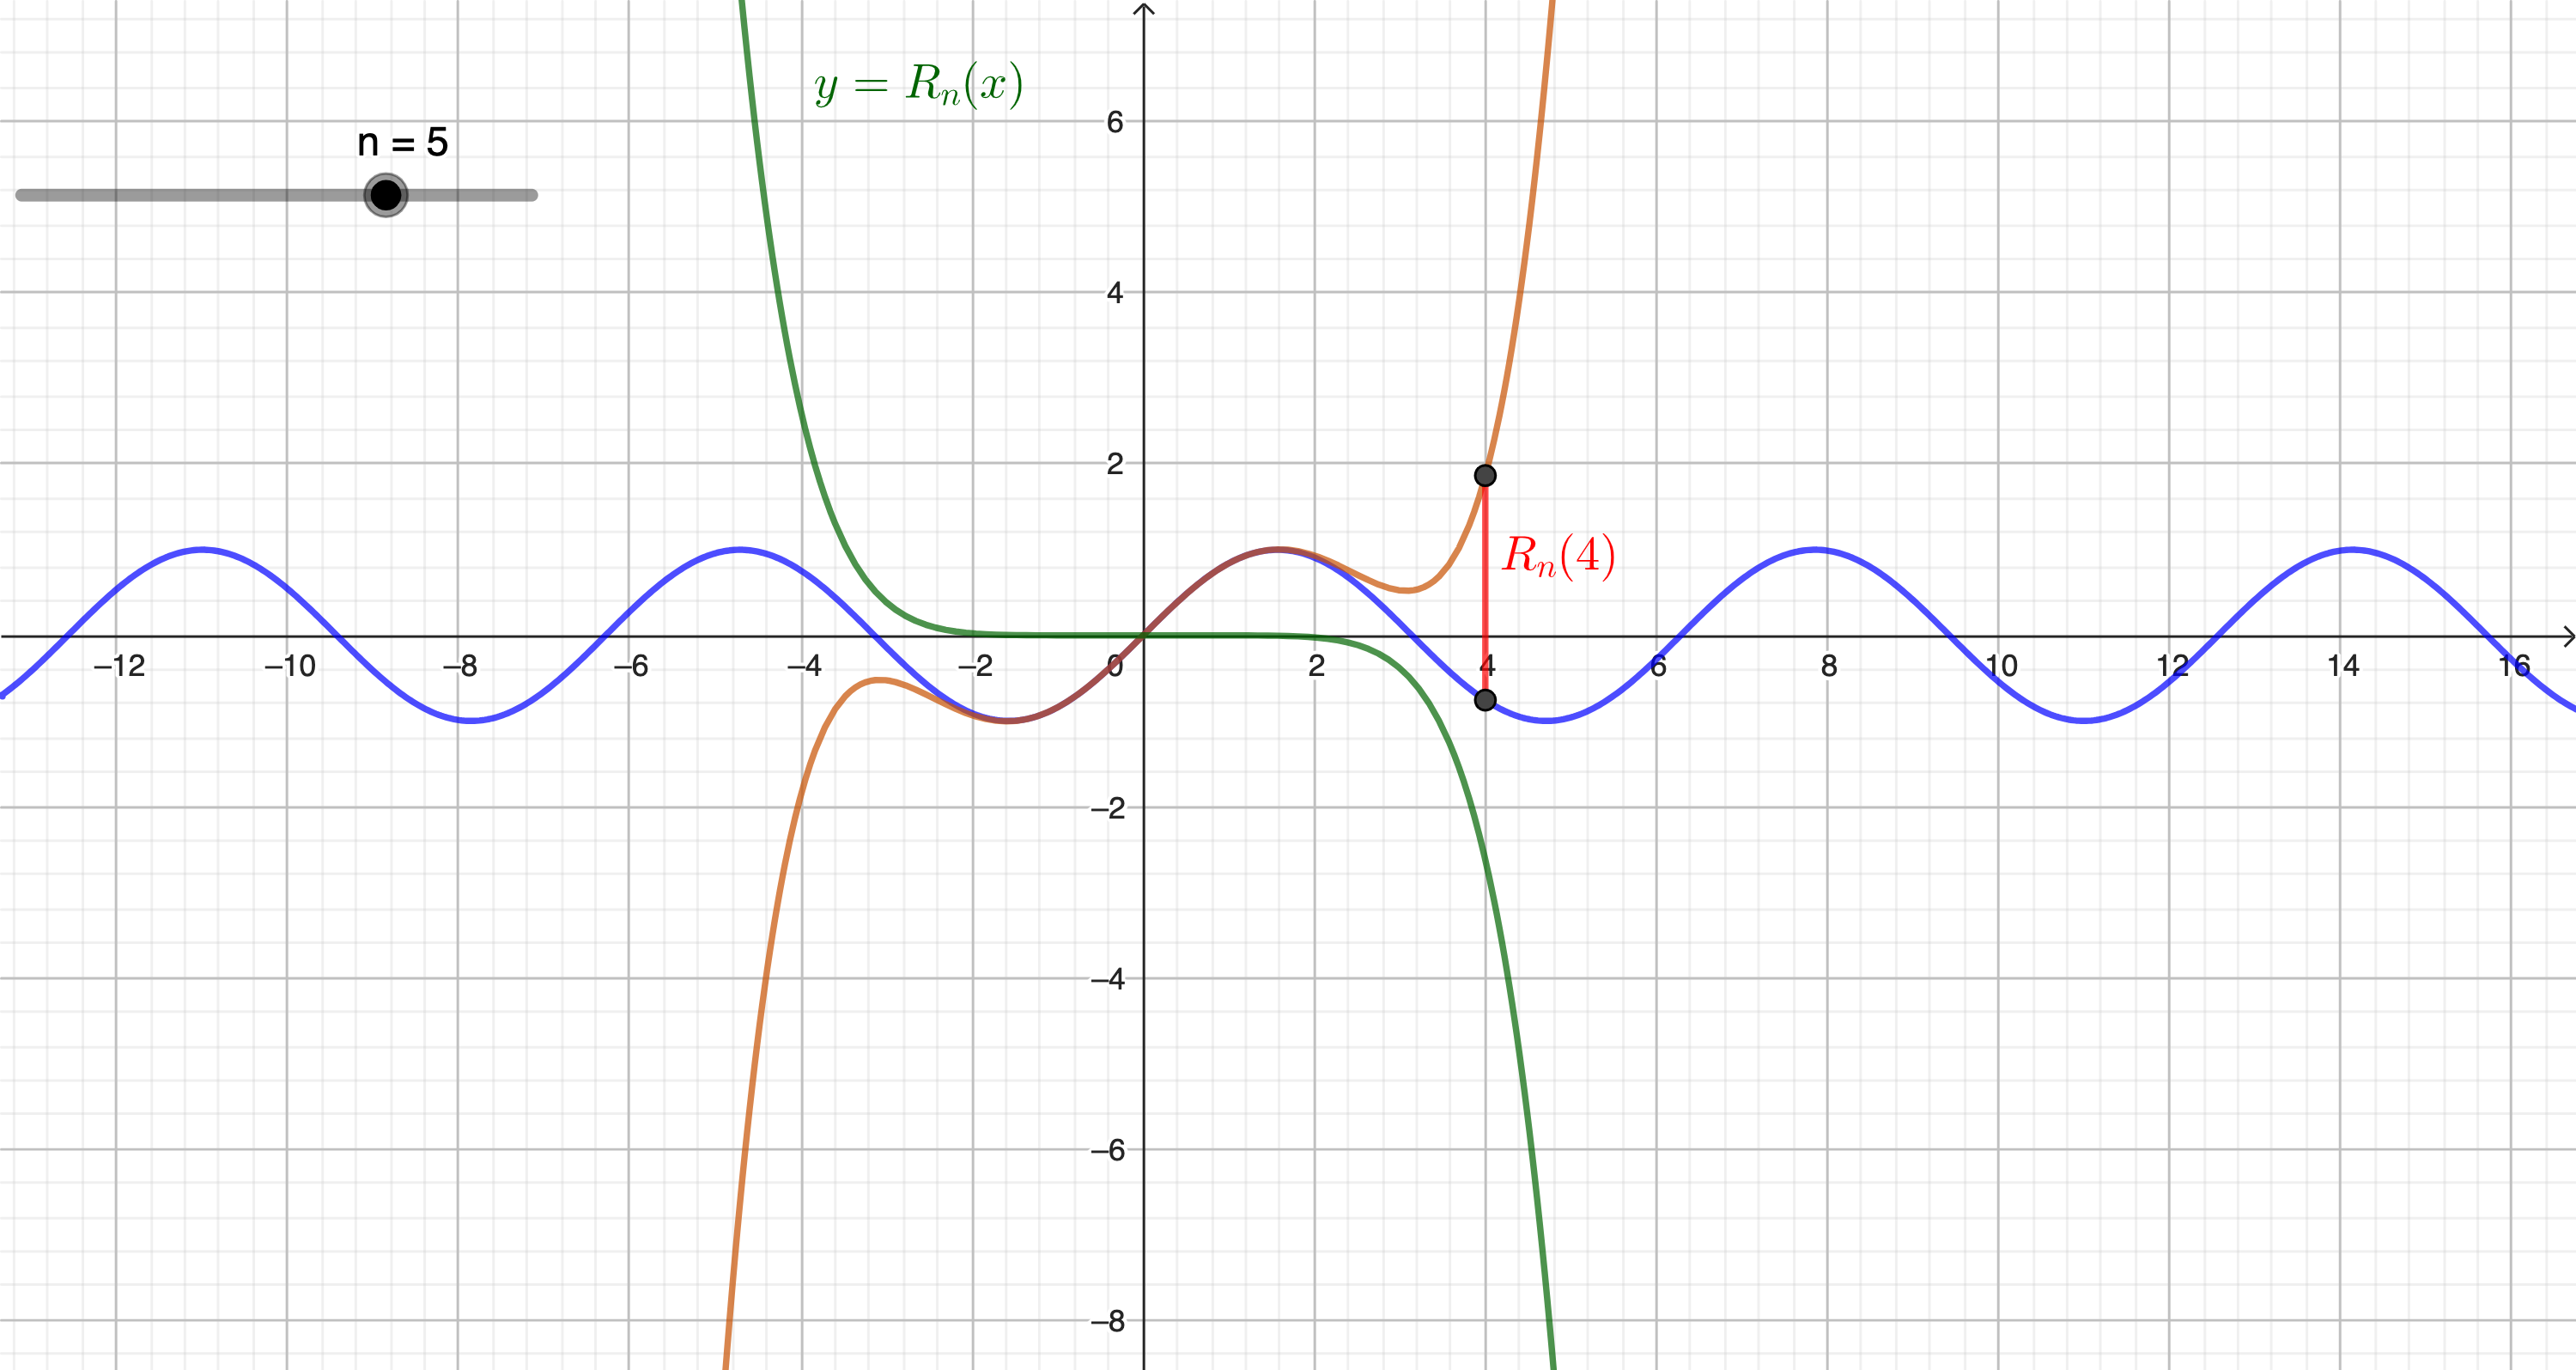
\includegraphics[width=0.45\textwidth]{media/restglied5.png}
	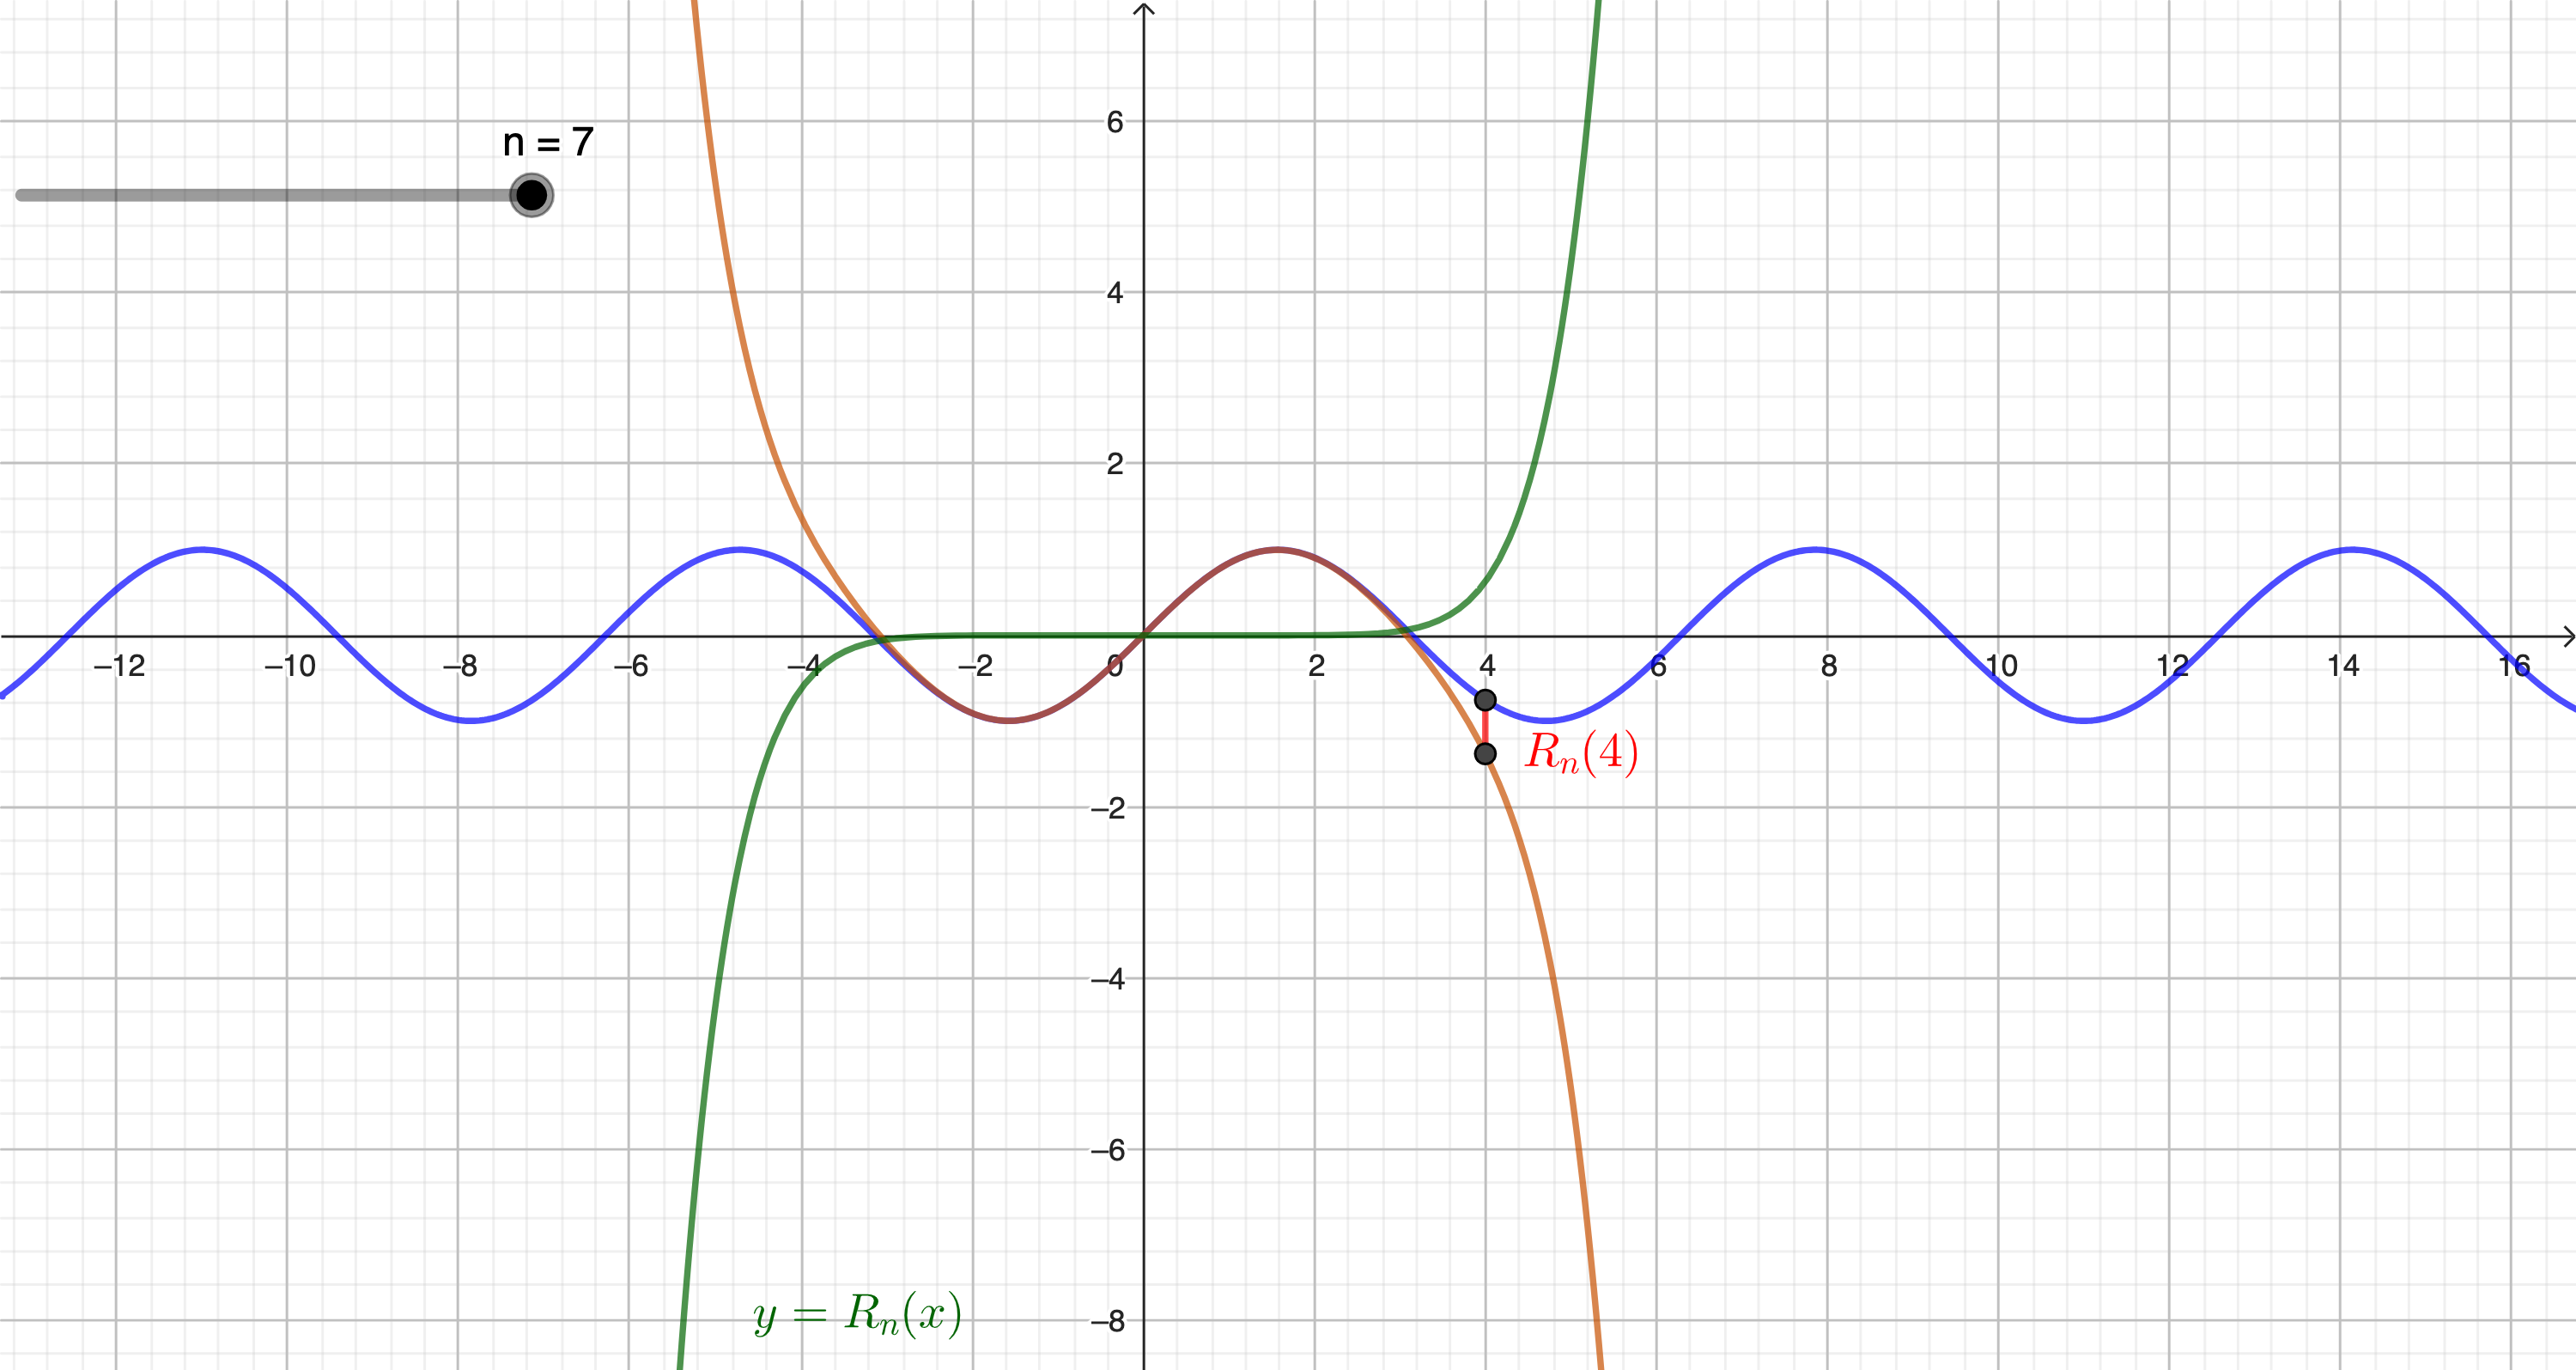
\includegraphics[width=0.45\textwidth]{media/restglied7.png}
	\caption{Restglied der Sinusfunktion für $n=1, 3, 5, 7$}
\end{figure}


Im Idealfall strebt die Abweichung $R_n(x)$ zwischen der Funktion $f$ und deren Taylorpolynom $T_n(x)$ für jeden Wert von $x$ gegen $0$.  Das ist bei der Sinusfunktion tatsächlich der Fall.

Um dies nachvollziehen zu können, werden wir den folgenden Weg beschreiten:
\begin{enumerate}
	\item Wir lernen den ersten Mittelwertsatz der Differentialrechnung kennen. Dabei handelt es sich um einen sogenannten Existenzsatz. Wir werden aber sehen, wie man aus solchen Sätzen konkrete Schlüsse ziehen kann.
	\item Mit dem  Mittelwertsatz werden wir eine Formel für die Berechnung des Restglieds $R_n(x)$ herleiten können. Damit lässt sich berechnen, wie genau eine Approximation durch ein Taylorpolynom ist.
	\item Schliesslich werden wir untersuchen, wie sich die Formel für das Restglied $R_n(x)$ verhält, wenn $n$ immer grösser wird. Damit können wir Beweisen, dass die Taylorreihen von $e^x, \sin(x), \cos(x)$ für $n\to\infty$ an jeder Stelle gegen die entsprechende Funktion konvergiert.
\end{enumerate}



\clearpage
%\input{mittelwertsatz.tex}

\subsection{Der Mittelwertsatz der Differentialrechnung}
In diesem Abschnitt werden wir
%den Zwischenwertsatz für stetige Funktionen und 
den ersten Mittelwertsatz der Differentialrechnung kennenlernen. Damit werden wir das Restglied der Taylorreihe abschätzen können.

\begin{LA}{}{MWS}
	Betrachten Sie den Graphen der Funktion $f(x) = x^3-x+3$ im Bereich $x\in[-2, 2]$.
	\begin{center}
		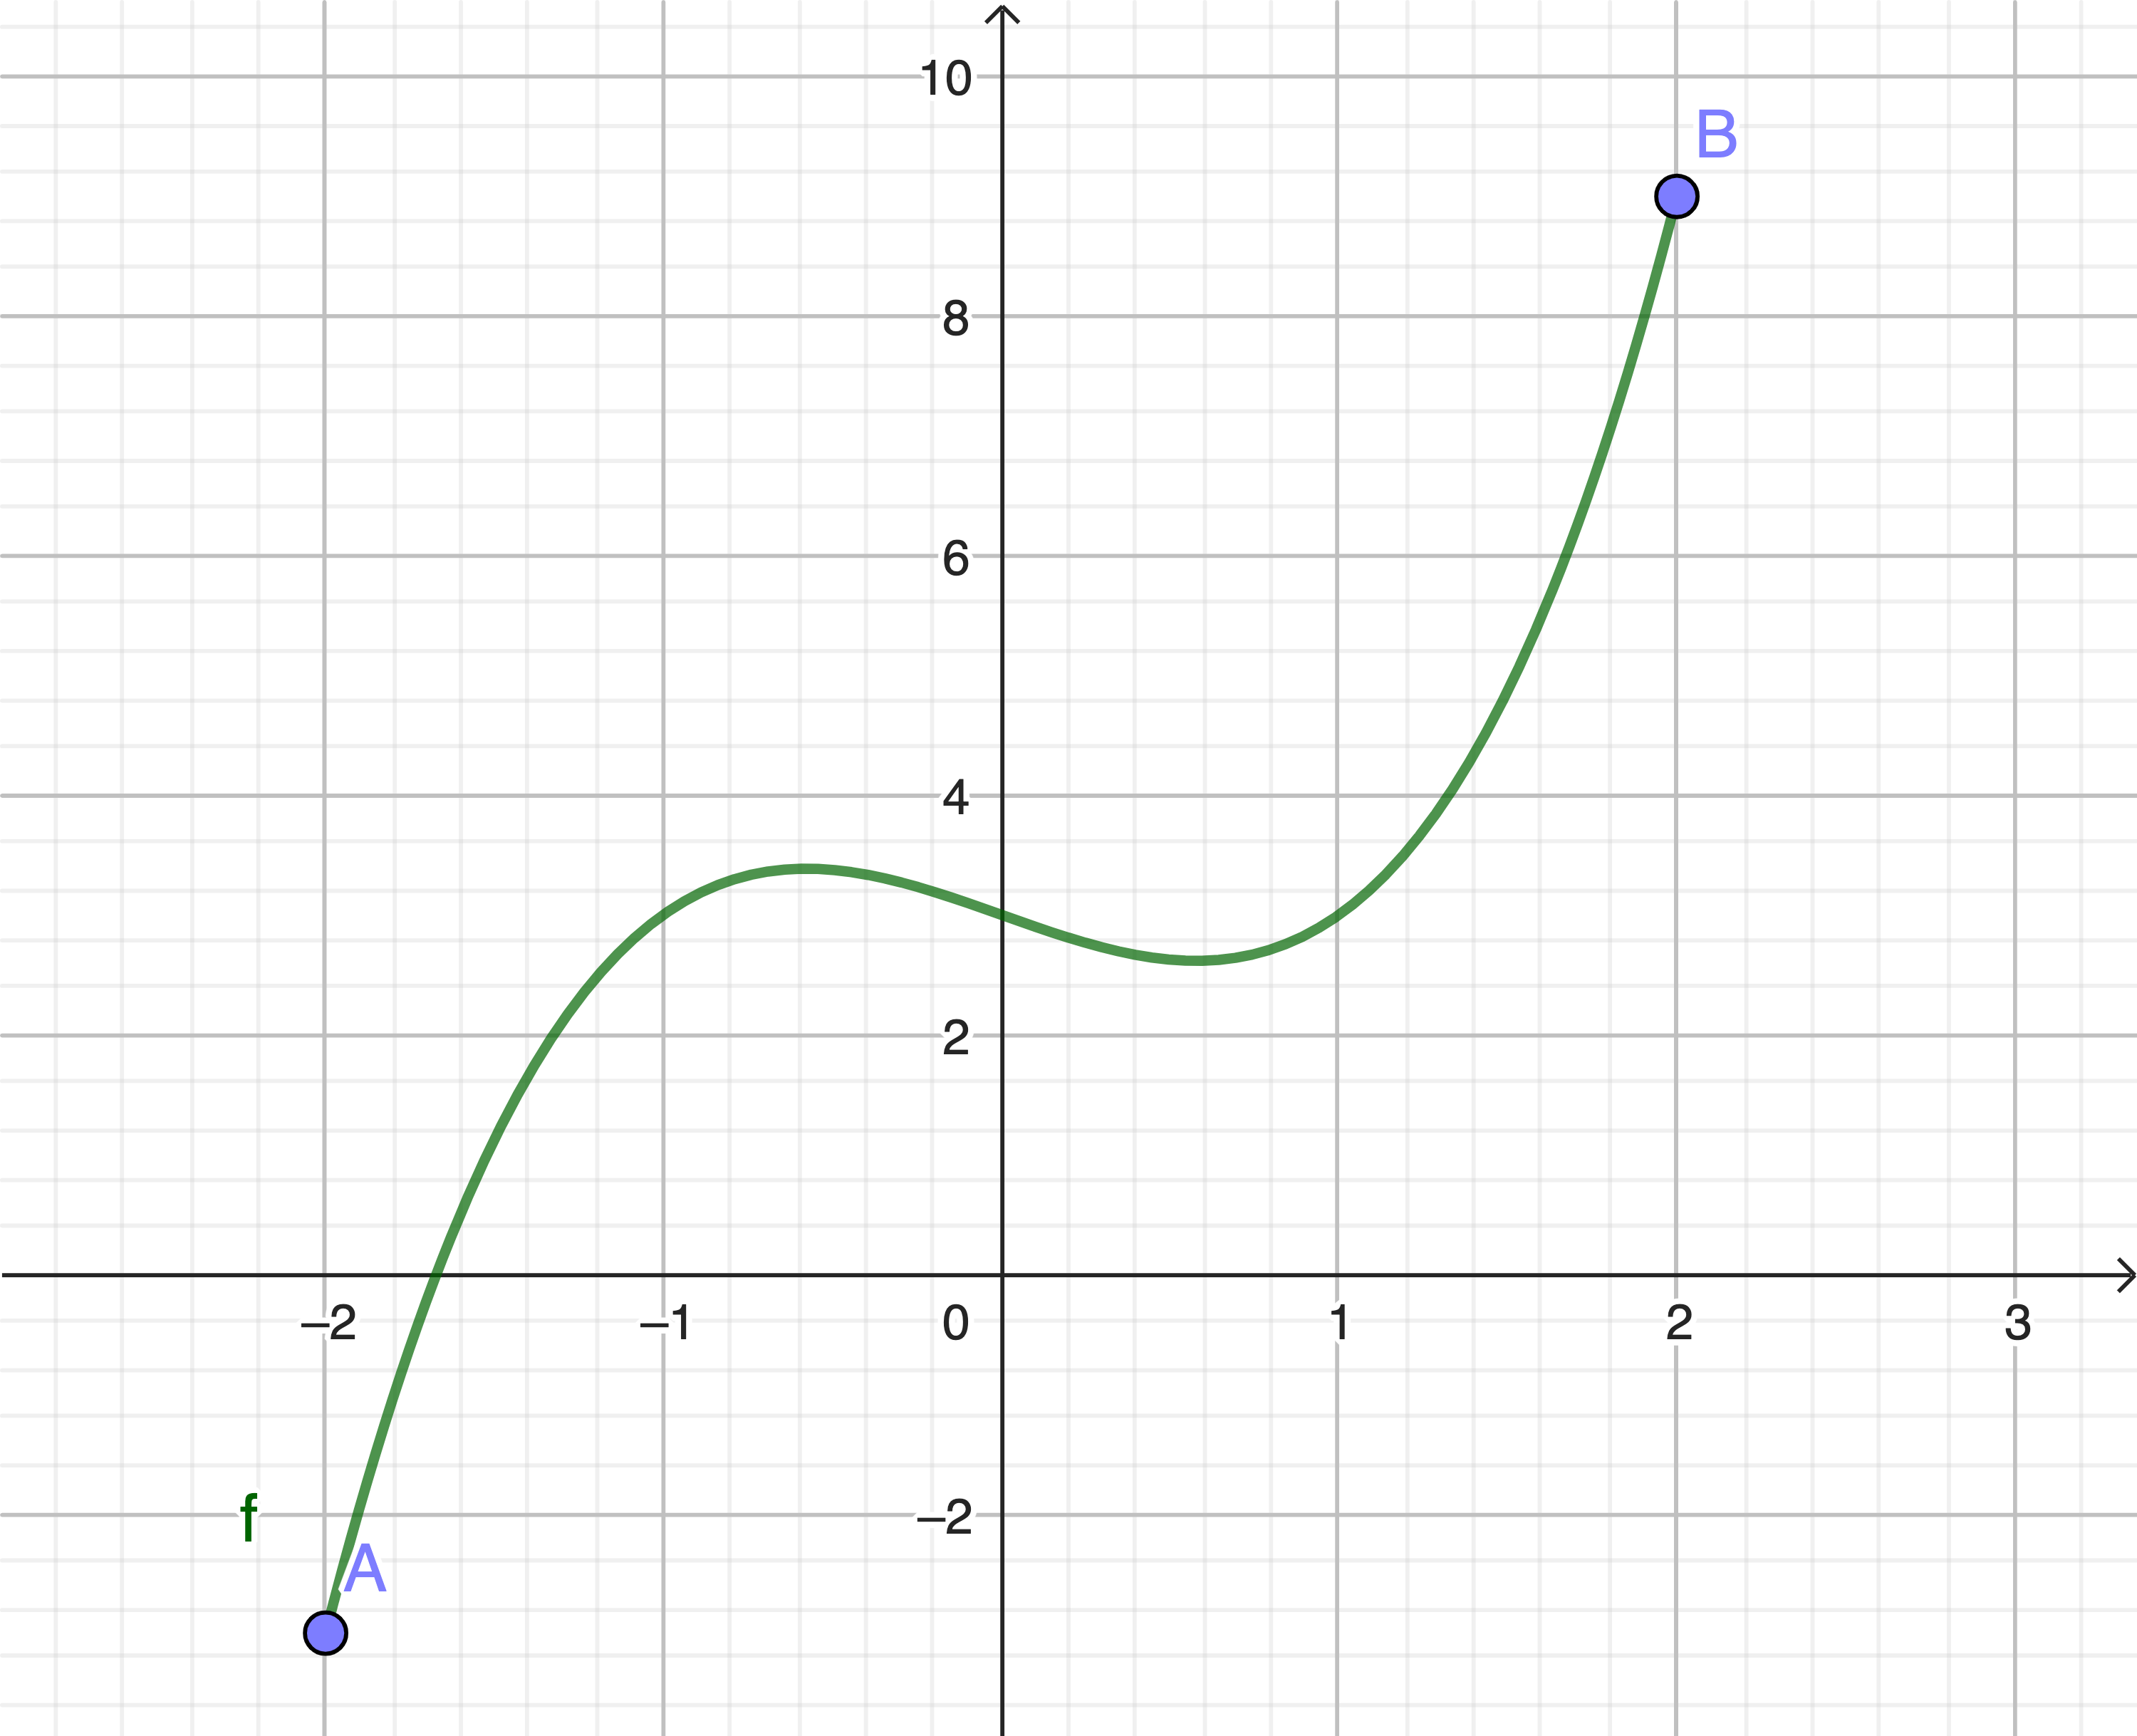
\includegraphics[width = 0.5 \textwidth]{media/LA-MWSV2.png}
	\end{center}

	\begin{enumerate}
		% \item Berechnen Sie den Wert des Quotienten 
		%     $$ \frac{\Delta y}{\Delta x} = \frac{f(2)-f(-2)}{2-(-2)} $$
		%     Welche geometrische Bedeutung hat dieser Zahl im Bezug auf den Graphen von $f$?
		\item Berechnen Sie die Steigung $m$ der Strecke zwischen den beiden Endpunkten $A$ und $B$ des Graphen von $f$.
		\item Schätzen Sie mit dem Graphen, an welchen Stellen der Graph von $f$ die Steigung $m$ aufweist.
		%\item Berechnen Sie den exakten Wert der Stellen, an welchen Stellen der Graph von $f$ die Steigung $m$ aufweist.
		\item Alice behauptet, sie kenne eine differenzierbare Funktion $f: \, [a,b] \rightarrow \R$ mit der Eigenschaft, dass
		      $$f'(x) > \frac{f(b)-f(a)}{b-a}$$
		      für alle $x\in [a,b]$.

		      Argumentieren Sie, wieso das nicht möglich ist.

	\end{enumerate}

\end{LA}

\clearpage

Die Überlegungen aus der Lernaufgabe können allgemein formuliert werden:

\begin{satz}{Erster Mittelwertsatz}{MWS1}
	Sei $f:[a,b]\longrightarrow \mathbb{R}$ eine stetig differenzierbare Funktion. Dann gibt es ein $c\in ]a,b[$ mit
	$$
		\frac{f(b)-f(a)}{b-a} \; = \; f'(c).
	$$
\end{satz}
Wir verzichten an dieser Stelle auf einen exakten Beweis des Satzes. Stattdessen werden wir ein anschauliches Argument liefern:

Die linke Seite der Gleichung im Satz $m = \frac{f(b)-f(a)}{b-a}$ ist die Steigung der Verbindungsstrecke $s$ zwischen den beiden Endpunkten $A=(a, f(a))$ und $B=(b, f(b))$ des Graphen. Diese kann auch interpretiert werden als die mittlere Steigung der Funktion $f$ im Intervall $[a,b]$.

Wenn die lokale Steigung $f'(x_1)$ an einer Stelle $x_1\in ]a,b[$ grösser als die mittlere Steigung $m$ ist, muss dieser Überschuss an einer anderen Stelle $x_2\in ]a,b[$ kompensiert werden.

In anderen Worten: wenn es eine Stelle $x_1$ gibt mit  $f'(x_1)>m$, muss es eine andere Stelle $x_2$ geben mit $f'(x_2) < m$. Da die Ableitungsfunktion $f'$ stetig ist (keine Sprünge aufweist), gibt es zwischen $x_1$ und $x_2$ mindestens eine Stelle $c$ mit $f'(c)=m$.
\begin{center}
	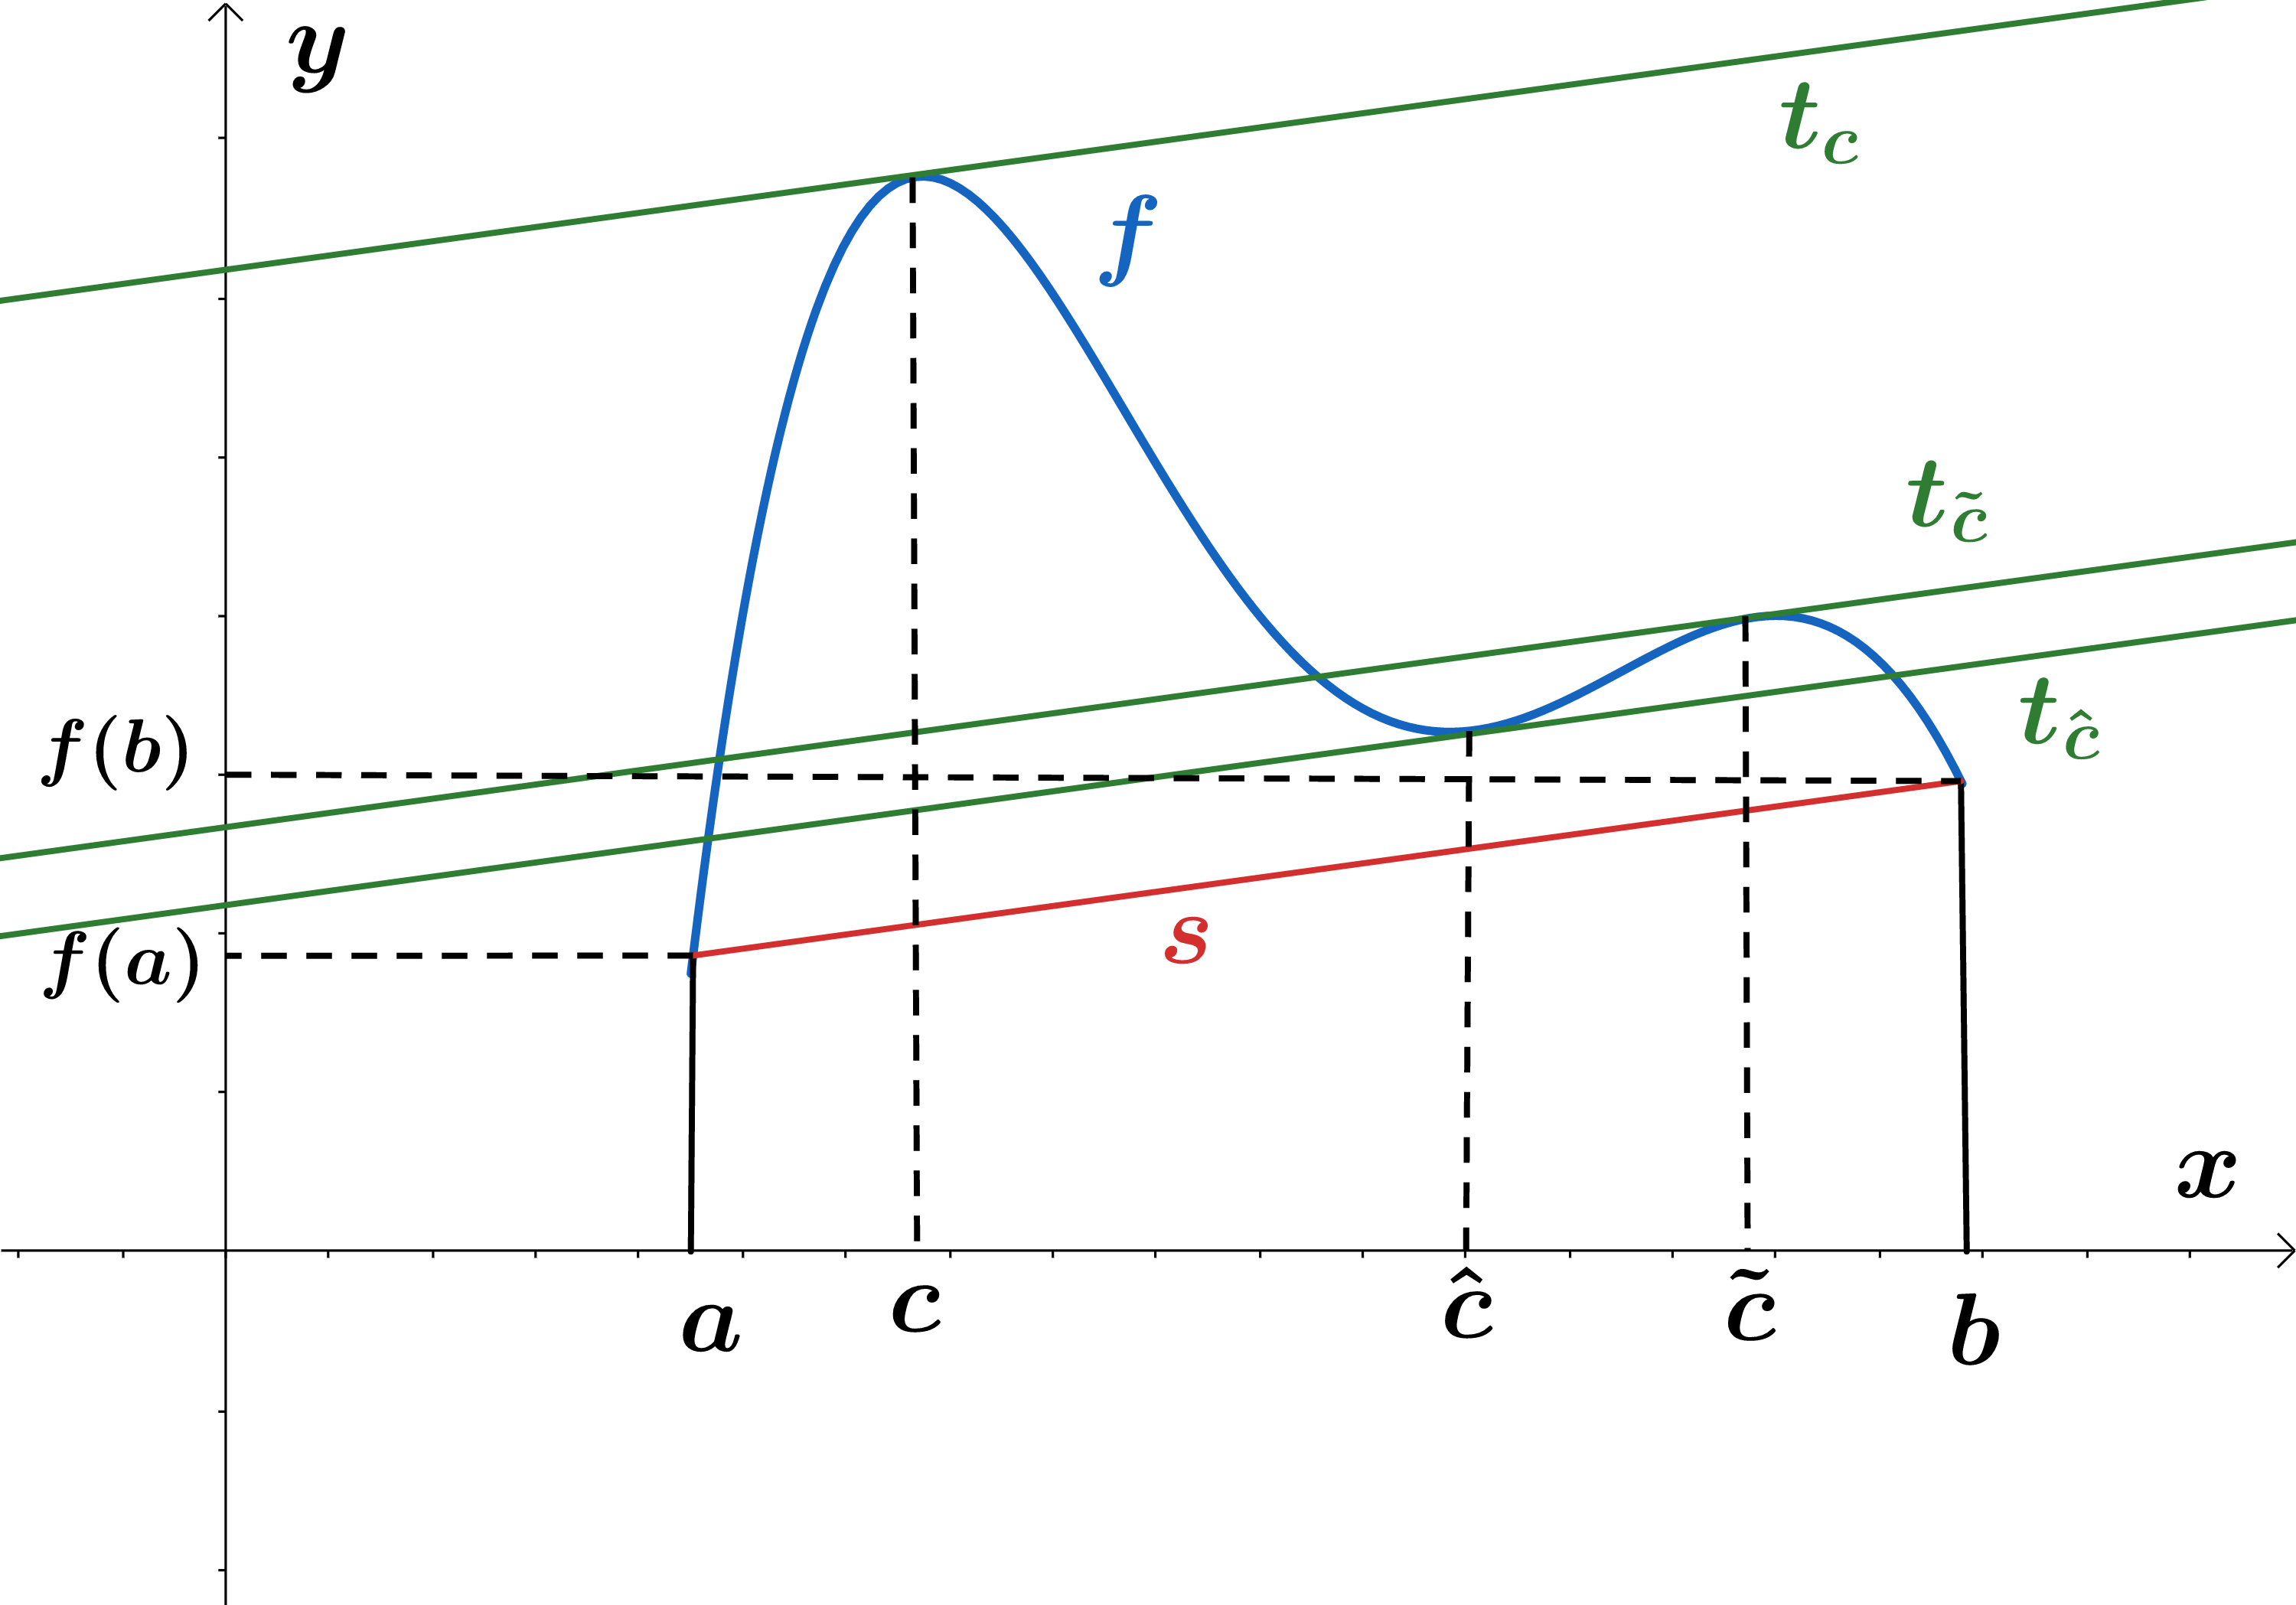
\includegraphics[width = 0.5 \textwidth]{media/mws.png}
\end{center}

Beim ersten Mittelwertsatz handelt es sich um einen sogenannten Existenzsatz. Er besagt zwar, dass eine Stelle $c\in ]a,b[$ mit
$
	\frac{f(b)-f(a)}{b-a} \; = \; f'(c)
$
existiert, gibt aber keine Anleitung, wie man diese Stelle finden kann. Auf den ersten Blick könnte man meinen, dass ein solcher Satz nicht sehr nützlich ist. Tatsächlich kann man aber damit konkrete Aussagen herleiten. Betrachten Sie dazu das folgende Beispiel. Dessen Aussage ist für uns nicht weiter wichtig. Es soll aber exemplarisch zeigen, wie man aus einem Existenzsatz eine konkrete Folgerung ziehen kann:
\clearpage
\begin{bsp}{Eine konkrete Anwendung des Mittelwertsatzes}{}
	Für jede positive Zahl $x > 0$ gilt $e^x > x+1$.
	\vspace{10cm}
	%Diese Ungleichung lässt sich mit dem ersten Mittelwertsatz herleiten.
\end{bsp}



\begin{ueb}{}{}
	Verwenden Sie den ersten Mittelwertsatz, um die folgende Ungleichung zu beweisen: Für alle $x>1$ gilt
	$$1 - \frac{1}{x} < \ln(x) < x-1$$

	Tipp: Die eine Ungleichung findet man, indem man das $c$  im Mittelwertsatz durch $1$ abschätzt, die andere, wenn man $c$ durch $x$ abschätzt.





\end{ueb}
% \clearpage
% \emph{Lösung}
% Das geht analog zum Beispiel. Die eine Ungleichung findet man, indem man das $c$  im Mittelwertsatz durch $1$ abschätzt, die andere, wenn man $c$ durch $x$ abschätzt.





%% Ausführliche Lösung - IGNORE %%
% Betrachte die Funktion \( f(t) = \ln(t) \) im Intervall \([1, x]\). Nach dem ersten Mittelwertsatz der Differentialrechnung gibt es ein \( c \in ]1, x[\) mit
% \[
% 	\frac{\ln(x) - \ln(1)}{x - 1} = \frac{1}{c}
% \]
% Daraus folgt
% \[
% 	\ln(x) = \frac{x}{c} - \frac{1}{c}
% \]
% Wegen \(1 < c < x\) folgt
% \[
% 	\frac{x}{x} - \frac{1}{x} < \ln(x) < \frac{x}{1} - \frac{1}{1}
% \]
% was zu beweisen war.



\clearpage
%\input{restgliedNachLagrange.tex}
\subsection{Das Restglied nach Lagrange}
In diesem Abschnitt werden mit dem Mittelwertsatz eine Formel für das $n$-te Restglied $R_n (x)=f(x)-T_n (x)$ der Taylorentwicklung herleiten. Damit werden wir beweisen können, dass einige der bereits hergeleiteten Taylorreihen tatsächlich gegen die ursprüngliche Funktion konvergieren. Ausserdem können wir mit dieser Formel den Fehler abschätzen, den man macht, wenn man einen Funktionswert durch den Wert des Taylorpolynoms $n$-ten Grades approximieren.

\textbf{Das Restglied $R_0(x)$}

Sei \( f \) eine differenzierbare Funktion und sei \( T_{0,x_0}(x) \) deren Taylorpolynom nullten Grades mit Entwicklungsstelle \( x_0 \), das heisst:
\[ T_{0,x_0}(x) = f(x_0) \]

Das Restglied \( R_0(x) \) ist dann die Differenz zwischen der Funktion \( f \) und der Taylorentwicklung \( T_{0,x_0}(x) \):
\[ R_0(x) = f(x) - T_{0,x_0}(x) = f(x) - f(x_0)\]
\begin{center}
	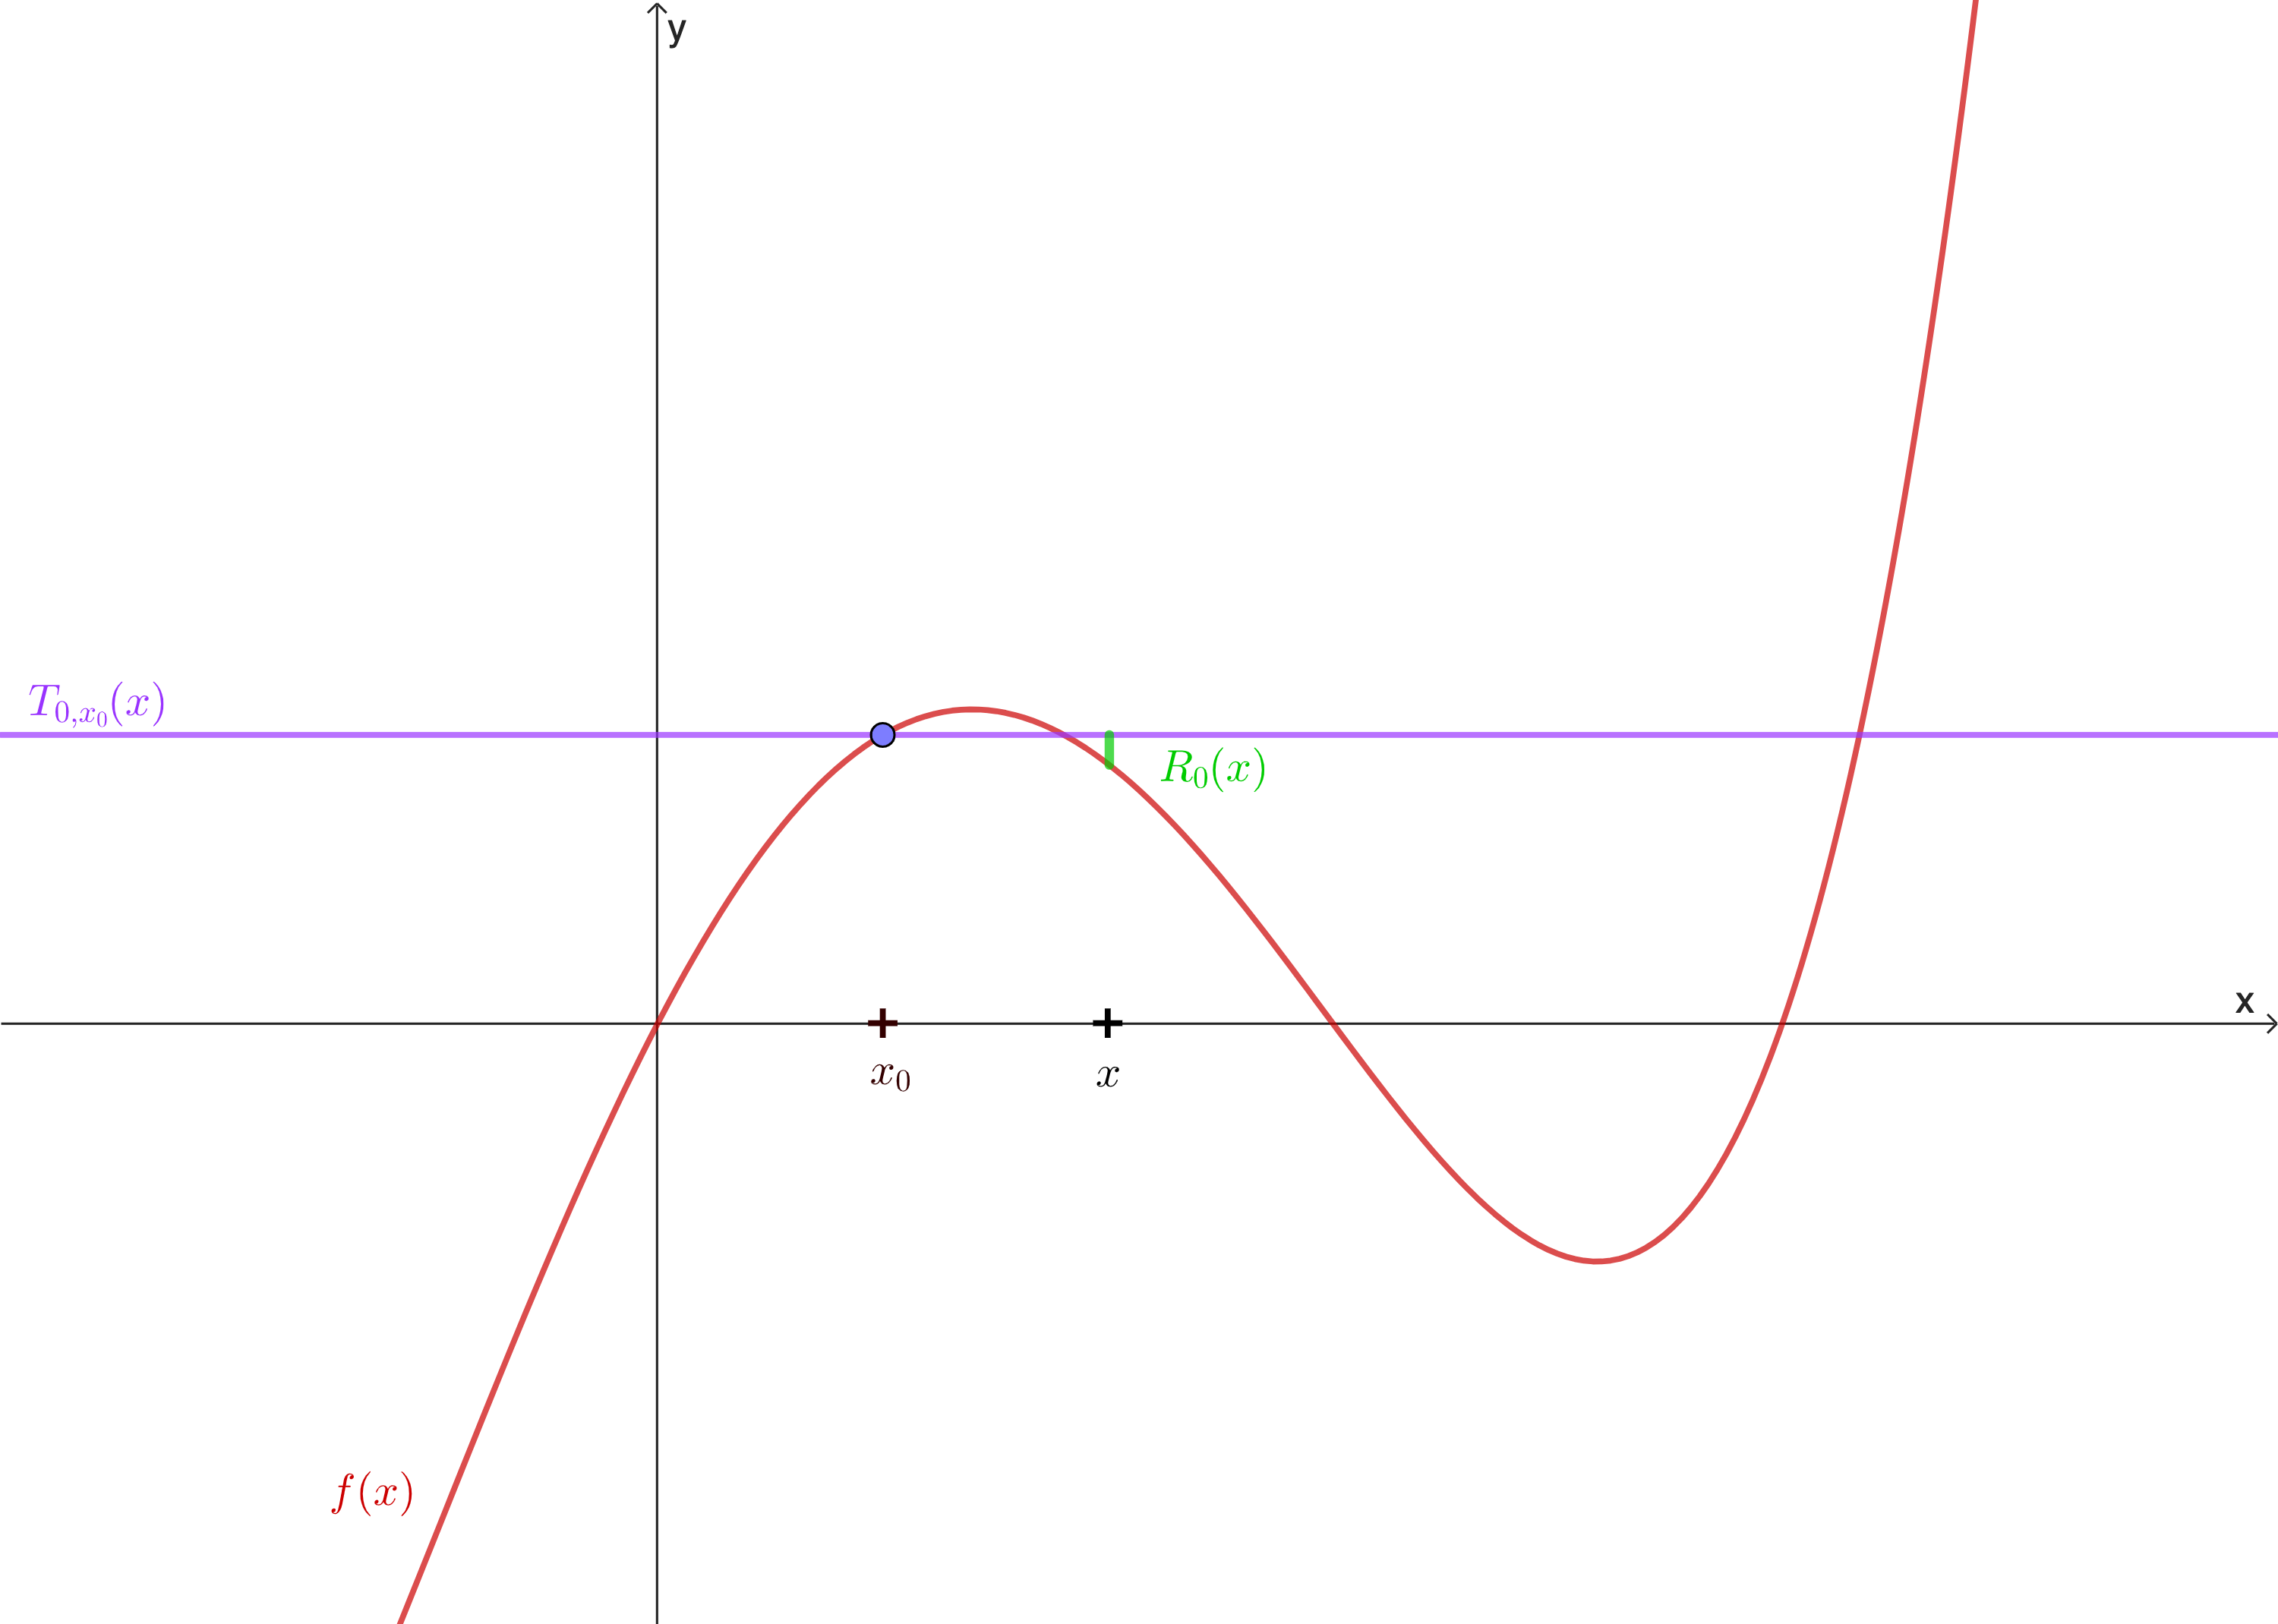
\includegraphics[width = 0.6 \textwidth]{media/BildRestglie0.png}
\end{center}

\begin{satz}
	{Restglied $R_0$ nach Lagrange}{}
	Sei $f$ stetig differenzierbar an der Stelle $x_0$. Für das 0. Restglied $R_0(x)$ der Taylorentwicklung gilt:
	$$R_0 (x)=  f'(c) \cdot (x-x_0)$$
	Für ein (nicht näher bekanntes) $c\in ]x_0, x[$.

\end{satz}
\begin{proof}

\end{proof}











\clearpage
% \textbf{Das Restglied $R_1(x)$}

% Sei \( f \) nun eine Funktion, die sich an der Stelle \( x_0 \) zweimal differenzieren lässt, und sei \( T_{1,x_0}(x) \) deren Taylorpolynom ersten Grades mit Entwicklungsstelle \( x_0 \), das heisst:
% \[ T_{1,x_0}(x) = f(x_0) + f'(x_0)(x - x_0) \]

% Das Restglied \( R_1(x) \) ist dann wieder die Differenz zwischen der Funktion \( f \) und der Taylorentwicklung \( T_{1,x_0}(x) \):
% \[ R_1(x) = f(x) - T_{1,x_0}(x) = f(x) - f(x_0) - f'(x_0)(x - x_0) \]
% \begin{center}
%     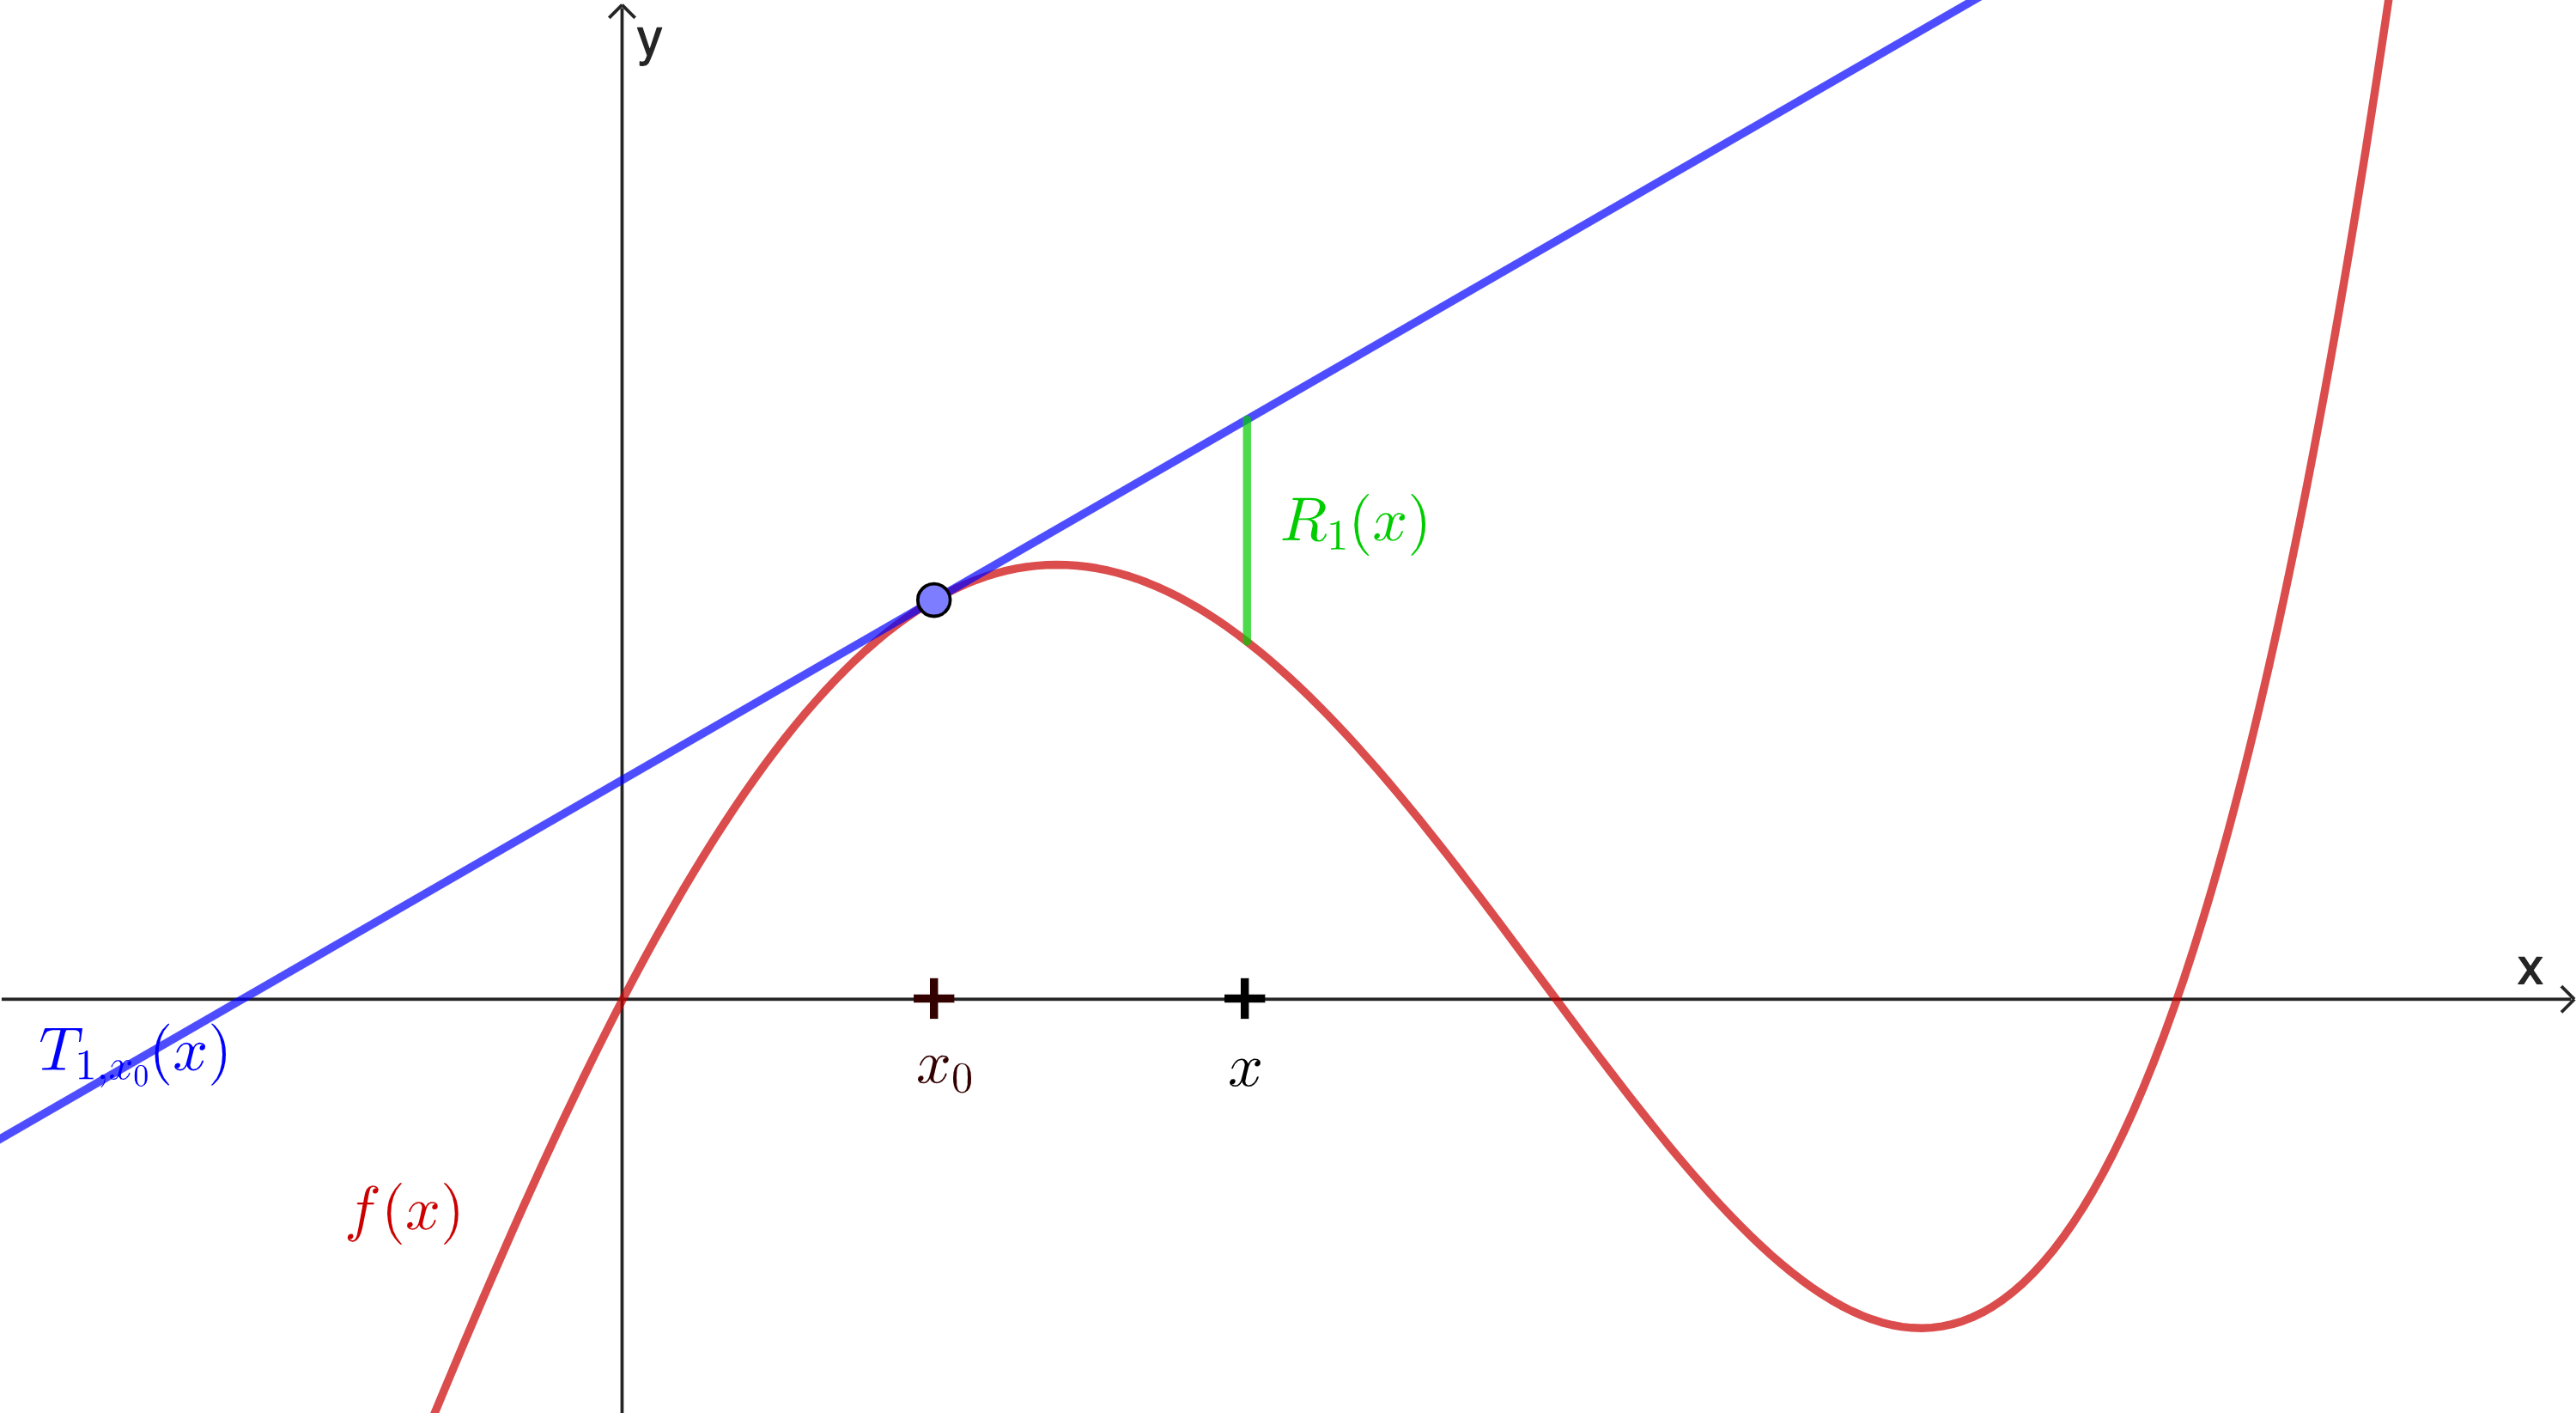
\includegraphics[width = 0.6 \textwidth]{media/BildRestglie1.png}
% \end{center}
% Nun wenden wir den 2. MWS auf die Funktionen $R_1 (x)$ und $g(x)=(x-x_0 )^2$ im Intervall $[x_0,x]$ an: (wird im Unterricht gemacht)
% \clearpage
% \begin{satz}
%     {Restglied $R_1$ nach Lagrange}{}
%     Sei $f$ zweimal stetig differenzierbar an der Stelle $x_0$. Für das 1. Restglied $$R_1 (x)=f(x)-T_{1,x_0 } (x)$$ gilt:
%     $$R_1 (x)= \qquad\qquad\qquad$$                                               

%     \vspace*{0.2cm}

% \end{satz}

% Mit dieser Formel für das Restglied kann man Abschätzen, welchen Fehler man macht, wenn man den Wert einer Funktion durch die konstante Approximation der Funktion annähert. 

% Versetzen Sie sich dazu in die Lage eines Ingenieurs in den Siebzigerjahre. Taschenrechner gibt es noch nicht. Um den Wert von $\sin(1^\circ)$ zu berechnen, verwendet er die Taylorapproximation 1. Grades. Der Fehler darf aber nicht grösser als $10^{-3}$ sein.  

% \begin{bsp}
%     {Fehler bei Approximation von $\sin(1^\circ)$ durch das Taylorpolynom 1. Grades (wird im Unterricht gemacht)}{} 

%     \vspace{13cm}
% %     Nutzen wir das Restglied von Lagrange einmal exemplarisch, um den Fehler abzuschätzen, den man macht, wenn man \(\sin(31^\circ)\) mithilfe der linearen Approximation der Sinusfunktion an der Stelle \(x_0 = 30^\circ\) annähert. Um besser ableiten zu können, müssen wir im Bogenmass rechnen: \(30^\circ \rightarrow \pi/6\), \(31^\circ \rightarrow 31\pi/180\), \(1^\circ \rightarrow \pi/180\).

% % Dann lautet das Taylorpolynom 1. Grades der Sinusfunktion an der Entwicklungsstelle \(x_0 = \pi/6\):
% % \[ T_{1,\pi/6}(x) = \sin(\pi/6) + \cos(\pi/6) \cdot (x-\pi/6) \]

% % Damit folgt für \(x = (31\pi)/180\):
% % \[ \sin(31^\circ) \approx T_{1,\pi/6}\left(\frac{31\pi}{180}\right) = \sin(\pi/6) + \cos(\pi/6) \cdot \left(\frac{31\pi}{180}-\pi/6\right) = \frac{1}{2} + \frac{\sqrt{3}}{2} \cdot \frac{\pi}{180} \approx 0.5151 \]

% % Den Fehler, den wir bei dieser Approximation machen, können wir nun mit dem Restglied nach Lagrange abschätzen:
% % \[ |R_1(31^\circ)| = |R_1(31\pi/180)| = \left|\frac{-\sin(c)}{2} \cdot \left(\frac{\pi}{180}\right)^2 \right| < \frac{1}{2} \cdot \left(\frac{\pi}{180}\right)^2 < 0.00015 \]

% \end{bsp}

Ähnlich wie die Formel für das 0. Restglied kann man auch jene für das $n$-te Restglied herleiten.
\begin{satz}
	{Restglied $R_n$ nach Lagrange}{}
	Sei \( f \) \((n+1)\)-mal stetig differenzierbar an der Stelle \( x_0 \). Für das \( n \)-te Restglied \( R_n(x) = f(x) - T_{n,x_0}(x) \) gilt:

	\[ R_n(x) = \frac{f^{(n+1)}(c)}{(n+1)!} \cdot (x - x_0)^{n+1} \]

	für ein (nicht näher bekanntes) \( c \in ]x, x_0[ \).

\end{satz}

In der Regel sorgt die Fakultät $(n+1)!$ im Nenner dafür, dass der Fehler für wachsendem $n$ immer kleiner wird. Man kann dann auch bestimmen, welcher Grad des Taylorpolynoms nötig ist, um eine bestimmte Genauigkeit zu garantieren.

\begin{bsp}
	{Approximation der Eulerschen Zahl $e$ mit vorgegebener Genauigkeit}{}
	Wir können wir Lagrange-Restglied verwenden, um die Zahl \(e\) mit einer Genauigkeit von \(10^{-6}\) zu berechnen. (Wird in der Klasse ergänzt)
	%    Dazu betrachten wir das Taylorpolynom \(n\)-ten Grades der Funktion \(e^x\) mit Entwicklungsstelle \(x_0 = 0\):
	% \[ T_n(x) = \sum_{k=0}^n \frac{x^k}{k!} \]
	% Für \(x = 1\) liefert uns \(T_n(1)\) eine Approximation für \(e\), wobei für den begangenen Fehler \(R_n(1) = e - T_n(1)\) nach Lagrange gilt: Es gibt ein \(c \in ]0, 1[\) mit
	% \[ R_n(1) = \frac{e^c}{(n+1)!} \cdot (1 - 0)^{n+1} = \frac{e^c}{(n+1)!} \]
	% Weil \(e^c < e^1 < 3\) ist, kann das Restglied grob abgeschätzt werden durch:
	% \[ R_n(1) < \frac{3}{(n+1)!} \]
	% Die angestrebte Genauigkeit von \(10^{-6}\) wird sicher erreicht, wenn
	% \[ |R_n(1)| < \frac{3}{(n+1)!} < 10^{-6} \implies 3 \cdot 10^6 < (n+1)! \implies n \geq 9 \]
	% Somit folgt, dass
	% \[ T_9(1) = \sum_{k=0}^9 \frac{1}{k!} = 1 + 1 + \frac{1}{2} + \frac{1}{6} + \frac{1}{24} + \frac{1}{120} + \frac{1}{720} + \frac{1}{5040} + \frac{1}{362880} =2.718281525573\ \]
	% sich um weniger als \(10^{-6}\) vom exakten Wert von $e$ unterscheidet.

	\vspace{13cm}

\end{bsp}
\clearpage
\begin{ueb}
	{}{}
	\begin{enumerate}
		\item 	Approximieren Sie den Wert von $f(x)$ durch das Taylorpolynom 1. Grades mit Entwicklungsstelle $x_0$. Schätzen Sie anschliessen den Fehler mit dem Lagrange-Restglied ab.
		      \begin{enumerate}
			      \item 	$f(x)=\ln(x), \, x_0=1, \,   x=1.01$
			      \item  	$f(x)=\frac{1}{\sqrt{x+1}}, \, x_0=0, \,   x=0.01$
			      \item  $f(x)=\sin(x), \, x_0=0,  \,  x= \frac{\pi}{180} \left(= 1^\circ\right)$
		      \end{enumerate}
		\item  	Bestimmen Sie das Taylorpolynom 3. Grades der Funktion $f(x)=\sin^2(x)=(\sin(x) )^2$ mit Entwicklungsstelle $x_0=0$ und zeigen Sie, dass dieses Polynom die Funktion $f$ im Intervall $\left[0,\frac{1}{2}\right]$ mit einer Genauigkeit von $\frac{1}{48}$ approximiert.

	\end{enumerate}
\end{ueb}
\clearpage
\emph{Lösungen:}
\begin{enumerate}
	\item  Approximationen
	      \begin{enumerate}
		      \item \( \ln(1.01) \approx 0.01, \,  |R_1(1.01)| < 0.00005 \)
		      \item \( f(0.01) \approx 0.995, \, |R_1(0.01)| < 3.75 \cdot 10^{-5} \)
		      \item  \( \sin\left(\frac{\pi}{180}\right) \approx \frac{\pi}{180} , \, \left|R_1\left(\frac{\pi}{180}\right)\right| < 0.00015 \)


	      \end{enumerate}

	\item Mit Kettenregel und Produktregel findet man: \( f'(0) = 0, f''(0) = 2, f'''(0) = 0 \).
	      Damit findet man \( T_3(x) = x^2 \).
	      Ausserdem ist \( |f^{(4)}(c)| = |8(1-2 \cos^2(c))| \leq 8 \implies \dots \implies |R_3(x)| \leq \frac{1}{48} \).


\end{enumerate}
\clearpage

\subsection{Konvergenz von Taylorreihen}

Mit der Formel für das $n$-te Restglied nach Lagrange können wir nun zeigen, dass die Taylorreihe der Sinusfunktion tatsächlich an jeder Stelle gegen $\sin(x)$ konvergiert. Dazu benötigen wir allerdings noch eine Zutat:
\begin{satz}
	{Fakultäten wachsen schneller als Exponentialfunktionen}{}
	\[\lim_{{n \to \infty}} \frac{|x|^n}{n!} = 0\] für jedes \(x \in \mathbb{R}\).

\end{satz}
\begin{proof}
	Die Folge \(a_n = \frac{|x|^n}{n!}\) kann rekursiv definiert werden als \(a_1 = x\), \(a_n = a_{n-1} \cdot \frac{|x|}{n}\). Wenn \(|x|\) sehr gross ist (z.B. \(|x| = 100\)), werden die ersten Glieder der Folge sehr schnell wachsen. Ab einem bestimmten Zeitpunkt wird \(n\) aber \(|x|\) überholen (z.B. ab dem 101. Glied). Danach werden die Folgenglieder immer kleiner. Sobald \(n > 2 \cdot |x|\) ist, werden die Folgenglieder jedes Mal mindestens halbiert. Damit konvergiert die Folge gegen Null.

\end{proof}
\begin{satz}
	{Konvergenz der Taylorentwicklung von $\sin(x)$}{}
	Die Taylorreihe \(T(x) = T_0(x) = \sum_{k=0}^{\infty} \frac{(-1)^k}{(2k+1)!} x^{2k+1}\) der Funktion \(f(x) = \sin(x)\) konvergiert für jedes \(x \in \mathbb{R}\) gegen \(f(x)\).

\end{satz}
\textit{Beweis:}

% \begin{proof}
%     \vspace{3cm}
% %     Für das \(n\)-te Restglied gibt es nach Lagrange ein \(c \in ]0, x[\):
% % \[ |R_n(x)| = \left| \frac{f^{(n+1)}(c)}{(n+1)!} \cdot x^{n+1} \right| =
% % \begin{cases}
% % \left| \frac{\cos(c)}{(n+1)!} \cdot x^{n+1} \right|, & \text{falls } n \text{ gerade} \\
% % \left| \frac{\sin(c)}{(n+1)!} \cdot x^{n+1} \right|, & \text{falls } n \text{ ungerade}
% % \end{cases} \leq \left| \frac{1}{(n+1)!} \cdot x^{n+1} \right| \]

% % Weil Fakultäten schneller wachsen als Exponentialfunktionen gilt nun:
% % \[ 0 \leq \lim_{{n \to \infty}} |R_n(x)| \leq \lim_{{n \to \infty}} \frac{x^{n+1}}{(n+1)!} = 0 \implies \lim_{{n \to \infty}} |R_n(x)| = 0 \]

% \end{proof}
\clearpage

\begin{ueb}
	{}{}
	\begin{enumerate}
		\item	Beweisen Sie, dass die Taylorreihe von $f(x)=e^x$ mit Entwicklungsstelle $x_0=0$ gegen $e^x$ konvergiert.

		\item Bei der Beschreibung von Hyperbeln spielen die Funktionen  $y= \frac{e^x - e^{-x}}{2}$ und $y= \frac{e^x + e^{-x}}{2}$ eine wichtige Rolle. Diese werden mit \emph{Hyperbelfunktionen} bezeichnet. Weil sie sich ausserdem in vielen Eigenschaften den trigonometrischen Funktionen ähneln, werden sie mit $\sinh(x) = \frac{e^x - e^{-x}}{2}$ (für \emph{sinus hyperbolicus}) und $\cosh(x)=\frac{e^x + e^{-x}}{2}$ (für \emph{cosinus hyperbolicus}) abgekürzt.
		      \begin{enumerate}
			      \item Zeigen Sie, dass für die Ableitungen der Hyperbelfunktionen gilt: \(\frac{d}{dx} \sinh(x) = \cosh(x)\) und \(\frac{d}{dx} \cosh(x) = \sinh(x)\). (Das ist eine erste Analogie zu den trigonometrischen Funktionen.)
			      \item Zeigen Sie, dass für die Hyperbelfunktionen die Gleichung \(\cosh^2(x) - \sinh^2(x) = 1\) gilt. (Das ist eine zweite Analogie zu den trigonometrischen Funktionen.)
			      \item         Bestimmen Sie die Taylorreihe der Funktion \(\sinh(x) = \frac{e^x - e^{-x}}{2}\) mit Entwicklungsstelle \(x_0 = 0\) und zeigen Sie, dass diese für alle \(x \in \mathbb{R}\) gegen \(\sinh(x)\) konvergiert.
		      \end{enumerate}


		\item Wie wir beobachtet haben, konvergiert die Taylorreihe der Funktion \(f(x) = \ln(x+1)\) in der Nähe der Entwicklungsstelle \(x_0 = 0\). Andererseits divergiert sie, wenn $x$ zu weit von $0$ entfernt ist. Diesem Phänomen soll in den folgenden Aufgaben nachgegangen werden.
		      \begin{enumerate}
			      \item Zeigen Sie, dass die Taylorreihe der Funktion \(f(x) = \ln(x+1)\) um $x_0 = 0$ für alle \(x\) im Bereich \(-\frac{1}{2} < x < \frac{1}{2}\) gegen \(f(x)\) konvergiert.
			      \item Was läuft an der Argumentation aus (a) schief, wenn man analog die Konvergenz für $x=2$ zeigen möchte?
		      \end{enumerate}


	\end{enumerate}
\end{ueb}
\clearpage
\emph{Lösungen:}
\begin{enumerate}

	\item Das Wesentliche: \( |R_n(x)| \leq \left|e^x \cdot \frac{x^{n+1}}{(n+1)!} \right| \rightarrow 0 \)



	\item
	      \begin{enumerate}
		      \item Folgt direkt mit der Kettenregel.
		      \item Lässt sich leicht aus der Definition und den binomischen Formeln herleiten.
		      \item Das Wesentliche: \( T(x) = \sum_{k=0}^n \frac{x^{2k+1}}{(2k+1)!} \), \( |R_n(x)| \leq \left|e^{|x|} \cdot \frac{x^{n+1}}{(n+1)!}\right| \rightarrow 0 \)
	      \end{enumerate}

	\item
	      \begin{enumerate}
		      \item Das ist etwas knifflig mit den Abschätzungen\dots

		            Das Wesentliche: \( |R_n(x)| \leq \frac{1}{n+1} \cdot \left(\frac{x}{c+1}\right)^{n+1} \leq \frac{1}{n+1} \cdot \left(\frac{\frac{1}{2}}{\frac{1}{2}}\right)^{n+1} \rightarrow 0\)
		      \item Für den Worst-Case $c=0$ erhält man die Abschätzung
		            $$|R_n(x)| \leq \frac{2^{n+1}}{n+1}$$
		            die für $n\to \infty$ nicht gegen Null strebt.
	      \end{enumerate}
\end{enumerate}


\begin{ueb}
	{Programmieraufgabe}{}
	Der folgende Python-Code berechnet eine Approximation für die Zahl $\sin(\pi/4)$ mit der Taylorentwicklung 19. Grades des Sinusfunktion.
	$$ \sin(x) \approx \sum_{i=0}^{9} \frac{(-1)^i}{(2i+1)!} \cdot x^{2i+1}$$
	\lstinputlisting{programme/sinus_approx.py}
	\begin{enumerate}
		\item Kopieren Sie den Code und lassen Sie ihn laufen.
		\item Berechnen Sie mit dem Programm eine Approximation für Winkel, die etwas weiter von $0$ entfernt sind und beobachten Sie, wie der Fehler zunimmt.
		\item Schreiben Sie ähnliche Programme zur Approximation anderer Funktionen, z.B. $\cos(x)$, $e^x$, $\ln(x)$, \dots
	\end{enumerate}
\end{ueb}

% \begin{ueb}
% 	{Programmieraufgabe für Experten}{}
% 	Schreiben Sie ein Python-Programm, dass die Taylorapproximation einer beliebigen Funktion an einer beliebigen Stelle bis zu einem gewünschten Grad berechnet.

% 	Einige Meilenteine:
% 	\begin{enumerate}
% 		\item Schreiben Sie ein Python-Funktion, die als Eingabe eine Funktion $f$ und eine Stelle $x_0$ erhält und eine Näherung für den Wert der Ableitung $f'(x_0)$ zurückgibt. Verwenden Sie dazu den Differenzenquotienten $\frac{f(x_0 + h) - f(x_0)}{h}$ mit einem kleinen $h$ (z.B. $h=10^{-5}$).
% 		\item Schreiben Sie eine Python-Funktion, die als Eingabe eine Funktion $f$, die Entwicklungsstelle $x_0$ und eine Stelle $x$ erhält und den Wert der Taylorapproximation 1. Grades mit Entwicklungsstelle $x_0$ von $f$ an der Stelle $x$ zurückgibt.
% 		\item Schreiben Sie eine Funktion , die als Eingabe eine Funktion $f$ erhält und die Ableitungsfunktion $f'$ zurückgibt. (Der Rückgabewert kann auch eine Python-Funktion sein!)
% 		\item Schreiben Sie ein Programm, das als Eingabe eine Funktion $f$ und eine Zahl $n$ erhält und die $n$-te Ableitung $f^{(n)}$ zurückgibt.
% 		\item Schreiben Sie nun eine Funktion, die als Eingabe eine Funktion $f$, die Entwicklungsstelle $x_0$, eine Stelle $x$ und einen Grad $n$ erhält und den Wert der Taylorapproximation $n$-ten Grades mit Entwicklungsstelle $x_0$ von $f$ an der Stelle $x$ zurückgibt.

% 	\end{enumerate}
% \end{ueb}

\clearpage
\section{Der Satz von Bernoulli / de l’Hôpital}
In diesem Abschnitt lernen wir eine nützliche Anwendung der Taylorreihen kennen, die es uns gestatten wird, viele Grenzwerte zu bestimmen, deren Berechnung sich bislang noch unseren Möglichkeiten entzieht.

Die Regeln von de l'Hôpital sind nach Guillaume François Antoine, Marquis de L'Hôpital benannt. L'Hôpital veröffentlichte sie 1696 in einem Lehrbuch der Differentialrechnung. Er hatte sie aber nicht selbst entdeckt, sondern von Johann Bernoulli gekauft, weshalb wir fairnesshalber auch Bernoullis Namen vermerken.



\subsection{Wiederholung Grenzwerte}
Im Grundlagenfach haben Sie sich mit Grenzwerten auseinandergesetzt. Wahrscheinlich haben Sie mit Grenzwerten von Folgen begonnen und die mathematische Definition mit Hilfe der $\varepsilon$-Umgebung gesehen. Danach haben Sie sich Grenzwerte für Funktionen für $x \to \pm\infty$ und $x \to a \in \mathbb{R}$ angeschaut. %Eventuell haben Sie dabei die $\epsilon$-$\delta$-Definition des Grenzwerts gesehen.

Sicher haben Sie dann aber auch die Grenzwertsätze und gewisse Faustregeln kennengelernt, die über die abstrakte Grenzwert-Definition hinaushelfen.

\begin{satz}
    {Grenzwertsätze}{}
    Existieren die Grenzwerte 
\[
\lim\limits_{x \to p} f(x) = a \quad \text{und} \quad \lim\limits_{x \to p} g(x) = b
\]
für \( p \in \mathbb{R}^* = \mathbb{R} \cup \{\pm\infty\} \), dann existieren auch die folgenden Grenzwerte und können wie angegeben berechnet werden.

Summe/Differenz:
\[
\lim\limits_{x \to p} \big(f(x) \pm g(x)\big) = \lim\limits_{x \to p} f(x) \pm \lim\limits_{x \to p} g(x) = a \pm b
\]

Produkt:
\[
\lim\limits_{x \to p} \big(f(x) \cdot g(x)\big) = \lim\limits_{x \to p} f(x) \cdot \lim\limits_{x \to p} g(x) = a \cdot b
\]

Division:  
Gilt zusätzlich \( b \neq 0 \), dann
\[
\lim\limits_{x \to p} \frac{f(x)}{g(x)} = \frac{\lim\limits_{x \to p} f(x)}{\lim\limits_{x \to p} g(x)} = \frac{a}{b}
\]
\end{satz}

\begin{satz}
    {Faustregeln}{}
    \[
\frac{\pm\infty}{c} = \pm\infty , 
\qquad
\frac{c}{\pm\infty} = 0
\]
\[
\frac{0}{c} = 0 , 
\qquad
\frac{c}{0} = \pm\infty
\]
\end{satz}

Aufpassen muss man, wenn eine unbestimmte Situation wie zum Beispiel 
\[
\frac{0}{0} \quad \text{oder} \quad \frac{\infty}{\infty}
\]
auftritt. In diesen Fällen muss der Term zuerst umgeformt werden. 

Bei diesen Situationen hilft manchmal Faktorisieren und Kürzen.

\begin{bsp}
    {}{}
\[
\lim\limits_{x \to \infty} \frac{3x^2 - x + 5}{x^2 + 5x + 4}
\]
\vspace{3cm}
\end{bsp}

\begin{bsp}
    {}{}
\[
\lim\limits_{x \to 5} \frac{x^2 - 3x - 10}{x - 5}
\]
\vspace{3cm}
\end{bsp}

%\clearpage
\begin{ueb}
    {}{}
    \begin{enumerate}
        \item $\lim\limits_{x \to \infty} \frac{1-x^2}{x}$
        \item $\lim\limits_{x \to \infty} \frac{3-x^3}{2x^3+x^2}$
        \item $\lim\limits_{x \to \infty} \frac{3x-21}{4x^2}$
        \item $\lim\limits_{x \to -2} \frac{x^2 - 2x - 8}{x^2 + 3x + 2}$
        \item $\lim\limits_{x \to 3} \frac{2x^2 - 6x}{x^2 + x - 12}$
    \end{enumerate}
\end{ueb}


\clearpage
\emph{Lösungen:}

\begin{enumerate}
    \item $\lim\limits_{x \to \infty} \frac{1-x^2}{x} = -\infty$
    \item $\lim\limits_{x \to \infty} \frac{3-x^3}{2x^3+x^2} = -\frac{1}{2}$
    \item $\lim\limits_{x \to \infty} \frac{3x-21}{4x^2} = 0$
    \item $\lim\limits_{x \to -2} \frac{x^2 - 2x - 8}{x^2 + 3x + 2} = 6$
    \item $\lim\limits_{x \to 3} \frac{2x^2 - 6x}{x^2 + x - 12} = \frac{6}{7}$
\end{enumerate}

















\clearpage
\subsection{Bernoulli / de L'Hôpital}

Wenn Zähler und Nenner der betrachteten Funktion keine Polynome sind, stösst man mit der Taktik   `Faktorisieren und Kürzen'  an Grenzen. Zum Beispiel lässt sich der Grenzwert $\lim_{x\rightarrow0} \frac{\sin(2x)}{x} $ auf diese Art nicht berechnen. Wir können die Berechnung solcher Grenzwerte aber mit Hilfe der Taylorpolynome angehen!

Seien $f$ und $g$ zwei Funktionen, die an der Stelle $x_0$ differenzierbar sind und für welche gilt: $f(x_0) = g(x_0) = 0$. Für die Berechnung des Grenzwertes $\lim_{x\rightarrow x_0} \frac{f(x_0)}{g(x_0)} $ kann man Zähler und Nenner durch ihre Taylorpolynome 1. Grades darstellen:
$$\frac{f(x)}{g(x)} = \frac{f(x_0) + f'(x_0)(x-x_0) + R^f_1(x)}{g(x_0) + g'(x_0)(x-x_0) + R^g_1(x)}$$
Weil nun $f(x_0) = g(x_0) = 0$ ist und mit dem Lagrange-Restglied folgt, dass es zwei Stellen $c_f, c_g \in [x_0, x]$ gibt, mit:
$$\frac{f(x)}{g(x)} = \frac{f'(x_0)(x-x_0) + \frac{f''(c_f)}{2} (x-x_0)^2}{ g'(x_0)(x-x_0) + \frac{g''(c_g)}{2}(x-x_0)^2}$$
Nun kann der Bruch mit $(x-x_0)$ gekürzt werden:
$$\frac{f(x)}{g(x)} = \frac{f'(x_0) + \frac{f''(c_f)}{2} (x-x_0)}{ g'(x_0) + \frac{g''(c_g)}{2}(x-x_0)}$$
Schliesslich findet man den Grenzwert
$$\lim_{{x \to x_0}} \frac{f(x)}{g(x)} = \frac{f'(x_0) + \frac{f''(c_f)}{2} (x_0-x_0)}{ g'(x_0) + \frac{g''(c_g)}{2}(x_0-x_0)} = \frac{f'(x_0)}{g'(x_0)}$$



% Die Taylorreihen können auch bei der Berechnung gewisser Grenzwerte nützlich sein:
% \begin{LA}{Grenzwerte $\lim_{x\rightarrow x_0} \frac{f(x)}{g(x)}$, wenn $f(x_0)=g(x_0)=0$}{}
%     \begin{enumerate}
%         \item Warm up: Berechnen Sie den Grenzwert $\lim_{x\rightarrow 0} \frac{3x^3+5x^2}{7x^5-2x^2}$.
%         \item In dieser Aufgabe soll der Grenzwert $\lim_{x\rightarrow 0} \frac{x-\sin(x)}{x^2(e^x-1)}$ ermittelt werden.
%         \begin{enumerate}
%             \item Wieso geht es nicht so wie in Aufgabe 1?
%             \item Ersetzen Sie die Funktion $\sin(x)$ durch ihre Taylorreihe $ \sin(x) = x-\frac{x^3}{3!}+\frac{x^5}{5!}- \ldots$ um die Entwicklungsstelle $x_0=0$ und vereinfachen Sie den Zähler von $\frac{x-\sin(x)}{x^2(e^x-1)}$ zu $$x-\sin(x) = \frac{x^3}{3!}-\frac{x^5}{5!}+\ldots $$
%             \item Gehen Sie mit dem Nenner gleich vor, um den Nenner zu vereinfachen zu $$x^2(e^x-1) = x^3+\frac{x^4}{2!}+\ldots $$
%             \item  Berechnen Sie nun den Grenzwert $$ \lim_{x\rightarrow 0} \frac{x-\sin(x)}{x^2(e^x-1)} = \lim_{x\rightarrow 0} \frac{\frac{x^3}{3!}-\frac{x^5}{5!}+\ldots }{ x^3+\frac{x^4}{2!}+\ldots }$$
%             indem Sie den Bruch mit $x^3$ kürzen.
%         \end{enumerate}
%         \item Gehen Sie gleich vor, wie in Aufgabe 2, um den folgenden Grenzwert zu bestimmen:
%         $$ \lim_{x\rightarrow 0} \frac{1-\cos(x)}{\sin^2(x)}$$
%     \end{enumerate}

% \end{LA}

 \begin{satz}
    {1. Regel von Bernoulli / de L'Hopital}{BH-1}
Seien $f$ und $g$ zwei Funktionen, die an der Stelle $x_0$ differenzierbar sind und für welche gilt: $f(x_0) = g(x_0) = 0$. Weiter sei $g'(x_0) \neq 0$. Dann folgt
\[
\lim_{{x \to x_0}} \frac{f(x)}{g(x)} = \frac{f'(x_0)}{g'(x_0)}
\]
 \end{satz}
%  \begin{proof}
%     Wie in der Lernaufgabe kann man Zähler und Nenner durch ihre Taylorpolynome 1. Grades darstellen:
%     $$\frac{f(x)}{g(x)} = \frac{f(x_0) + f'(x_0)(x-x_0) + R^f_1(x)}{g(x_0) + g'(x_0)(x-x_0) + R^g_1(x)}$$
%     Weil nun $f(x_0) = g(x_0) = 0$ ist und mit dem Lagrange-Restglied folgt, dass es zwei Stellen $c_f, c_g \in [x_0, x]$ gibt, mit:
%     $$\frac{f(x)}{g(x)} = \frac{f'(x_0)(x-x_0) + \frac{f''(c_f)}{2} (x-x_0)^2}{ g'(x_0)(x-x_0) + \frac{g''(c_g)}{2}(x-x_0)^2}$$
%     Nun kann der Bruch mit $(x-x_0)$ gekürzt werden:
%     $$\frac{f(x)}{g(x)} = \frac{f'(x_0) + \frac{f''(c_f)}{2} (x-x_0)}{ g'(x_0) + \frac{g''(c_g)}{2}(x-x_0)}$$
%     Schliesslich findet man den Grenzwert
%     $$\lim_{{x \to x_0}} \frac{f(x)}{g(x)} = \frac{f'(x_0) + \frac{f''(c_f)}{2} (x_0-x_0)}{ g'(x_0) + \frac{g''(c_g)}{2}(x_0-x_0)} = \frac{f'(x_0)}{g'(x_0)}$$


%  \end{proof}
 
 \begin{bsp}
    {}{}
    $$\lim_{x\rightarrow0} \frac{\sin(2x)}{x} = ? $$

    \vspace{3cm}

    % Zähler und Nenner streben beide gegen $0$, womit die Voraussetzungen für den Satz von Bernoulli/de L’Hôpital erfüllt sind. 
    %  $$\lim_{x\rightarrow0} \frac{\sin(2x)}{x} \stackrel{\text{(BH)}}{=}  \frac{\cos(2 \cdot 0)\cdot 2}{1} = 2 $$ 
 \end{bsp}
 \begin{bsp}
    {}{}
    Die Regel von Bernoulli / de l’Hôpital darf auch mehrmals angewendet werden.
    \[
\lim_{{x \to 0}} \frac{{x - \sin(x)}}{{x^3}} =?
\]
% \[
% \lim_{{x \to 0}} \frac{{x - \sin(x)}}{{x^3}} \overset{(\text{BH})}{=}
% \lim_{{x \to 0}} \frac{{1 - \cos(x)}}{{3x^2}} \overset{(\text{BH})}{=} 
% \lim_{{x \to 0}} \frac{{\sin(x)}}{{6x}} \overset{(\text{BH})}{=} 
% \lim_{{x \to 0}} \frac{{\cos(x)}}{{6}} = \frac{1}{6}
% \]
\vspace{3cm}

 \end{bsp}

 \begin{bsp}
    {Die Voraussetzungen sind wichtig!}{}
    \[
\lim_{{x \to 0}} \frac{x}{e^x} = ?
\]
Achtung: Hierbei handelt es sich um einen Grenzwert vom Typ $0/1$. Die Voraussetzungen für den Satz von Bernoulli / de L'Hôpital sind damit nicht gegeben. Offensichtlich gilt
\[
\lim_{{x \to 0}} \frac{x}{e^x} = \frac{0}{1} =0
\]
Wird BH fälschlicherweise verwendet, erhält man das falsche Resultat:
\[
\lim_{{x \to 0}} \frac{x}{e^x} \neq \lim_{{x \to 0}} \frac{1}{e^x} = 1 
\]
 \end{bsp}


\begin{ueb}
    {Zu Bernoulli / de l'Hôpital 1}{}


 \begin{enumerate}
    \item Bestimmen Sie folgende Grenzwerte nach der 1. Regel von Bernoulli / de l'Hôpital:
    \begin{enumerate}
        %\item $\lim\limits_{x \to a} \frac{x - a}{\sin(x - a)}$
        \item $\lim\limits_{x \to \frac{\pi}{2}} \frac{\cos(x)}{\frac{\pi}{2} - x}$
        \item $\lim\limits_{x \to 0} \frac{x^2 - \sin (x)}{x^2 + \sin x}$
        \item $\lim\limits_{x \to 0} \frac{\sin(x) + x}{\sin x}$
        \item $\lim\limits_{x \to 0} \frac{x \cdot \sin(x)}{x^2 - \sin(x)}$. Denken Sie an die Produktregel!
        %\item $\lim\limits_{x \to \frac{\pi}{2}} \frac{(x - \frac{\pi}{2}) \cdot \sin x}{\cos x}$
        \item $\lim\limits_{x \to 0} \frac{\sin(x^2)}{x}$. Denken Sie an die Kettenregel!
    \end{enumerate}
    
    \item Diese Grenzwerte können sowohl mit `Faktorisieren und Kürzen' als auch mit der 1. Regel von Bernoulli / de l'Hôpital bestimmt werden. Wählen Sie einen passenden Lösungsweg und berechnen Sie den Grenzwert.
    \begin{enumerate}
        \item $\lim\limits_{x \to -2} \frac{x^2 - x - 6}{x + 2}$
        \item $\lim\limits_{x \to -1} \frac{x^2 + x}{x + 1}$
        \item $\lim\limits_{x \to 1} \frac{x^3+x^2 + x - 3}{x - 1}$
        
        %\item $\lim\limits_{x \to 1} \frac{x^3 - 1}{x - 1}$
        \item $\lim\limits_{x \to 5} \frac{x^{10} - 5^{10}}{x^7 - 5^7}$
        %\item $\lim\limits_{x \to -4} \frac{x^3 + 4^3}{x^8 - 4^8}$
    \end{enumerate}
    
    %\item Bestimmen Sie die Grenzwerte aus 4 a)-d) ohne die 1. Regel von Bernoulli / de l'Hôpital:
    
    \item Warum darf man bei $\lim\limits_{x \to 2} \frac{x^2 - x + 2}{x - 2}$ die 1. Regel von Bernoulli / de l'Hôpital nicht anwenden?
   Was würde sich nach dieser Regel ergeben? Zeigen Sie, dass der Grenzwert nicht existiert.

    
    
    \item Mehrfache Anwendung der Regel von Bernoulli / de l'Hôpital
    \begin{enumerate}
        \item $\lim\limits_{x \to 5} \frac{3x^2 - 30x + 75}{7x^2 - 70x + 175}$.
        \item $\lim\limits_{x \to 0} \frac{1 - \cos(x)}{x^2}$.
        \item $\lim\limits_{x \to 0} \frac{\sin^2(x)}{x^2}$.
    \end{enumerate}
\end{enumerate}

\end{ueb}
\clearpage
\emph{Lösungen:}

\begin{enumerate}
    \item Bestimmen Sie folgende Grenzwerte nach der 1. Regel von Bernoulli / de l'Hôpital:
    \begin{enumerate}
        %\item $\lim\limits_{x \to a} \frac{x - a}{\sin(x - a)} = 1$
        \item $\lim\limits_{x \to \frac{\pi}{2}} \frac{\cos x}{\frac{\pi}{2} - x} = 1$
        \item $\lim\limits_{x \to 0} \frac{x^2 - \sin x}{x^2 + \sin x} = -1$
        \item $\lim\limits_{x \to 0} \frac{\sin x + x}{\sin x} = 2$
        \item $\lim\limits_{x \to 0} \frac{x \cdot \sin(x)}{x^2 - \sin(x)} = 0 $. Denken Sie an die Produktregel!
        %\item $\lim\limits_{x \to \frac{\pi}{2}} \frac{(x - \frac{\pi}{2}) \cdot \sin x}{\cos x} = -1$
        \item $\lim\limits_{x \to 0} \frac{\sin(x^2)}{x} = 0$. Denken Sie an die Kettenregel!
    \end{enumerate}
    
    \item Diese Grenzwerte können sowohl mit `Faktorisieren und Kürzen' als auch mit der 1. Regel von Bernoulli / de l'Hôpital bestimmt werden. Wählen Sie einen passenden Lösungsweg und berechnen Sie den Grenzwert.
    \begin{enumerate}
        \item $\lim\limits_{x \to -2} \frac{x^2 - x - 6}{x + 2} = -5$
        \item $\lim\limits_{x \to -1} \frac{x^2 + x}{x + 1} = -1$
        \item $\lim\limits_{x \to 1} \frac{x^3+x^2 + x - 3}{x - 1} = 6$
        
        %\item $\lim\limits_{x \to 1} \frac{x^3 - 1}{x - 1} = 3$
        \item $\lim\limits_{x \to 5} \frac{x^{10} - 5^{10}}{x^7 - 5^7} = \frac{1250}{7}$
        %\item $\lim\limits_{x \to -4} \frac{x^3 + 4^3}{x^8 - 4^8} = -\frac{3}{8192}$
    \end{enumerate}
    
    %\item Bestimmen Sie die Grenzwerte aus 4 a)-d) ohne die 1. Regel von Bernoulli / de l'Hôpital:
    
    \item Es handelt sich nicht um den Fall $\frac{0}{0}$ sondern $\frac{4}{0}$ Der (uneigentliche) Grenzwert ist daher $\lim\limits_{x \to 2} \frac{x^2 - x + 2}{x - 2} = \pm\infty$. (Genauer: $\lim\limits_{x \uparrow 2} = -\infty$ und $\lim\limits_{x \downarrow 2} = \infty$  ) Würde man die Regel fälschlicherweise anwenden erhielte man: $3$.

    
    
    \item Mehrfache Anwendung der Regel von Bernoulli / de l'Hôpital
    \begin{enumerate}
        \item $\lim\limits_{x \to 5} \frac{3x^2 - 30x + 75}{7x^2 - 70x + 175} = \frac{3}{7}$.
        \item $\lim\limits_{x \to 0} \frac{1 - \cos x}{x^2} = \frac{1}{2}$.
        \item $\lim\limits_{x \to 0} \frac{\sin^2 x}{x^2} = 1$.
    \end{enumerate}
\end{enumerate}

  











\clearpage
 Es gibt noch weitere Varianten und Versionen der Regel von Bernoulli / de L'Hôpital. Die Grundaussage ist dabei jeweils sehr ähnlich. Unter bestimmten Bedingungen dürfen wir im Zähler und im Nenner ableiten. Erhalten wir damit einen bestimmten Ausdruck, so haben wir den ursprünglich gesuchten Grenzwert gefunden.
 
 \begin{satz}
    {Varianten von Bernoulli / de L'Hôpital}{BH-Varianten}
    \begin{enumerate}
        \item Fall $\frac{0}{0}$ für $x \rightarrow x_0$ (Das ist die Variante von oben, angepasst für mehrfache Anwendung)
        
        Seien $f$ und $g$ zwei Funktionen, die an der Stelle $x_0$ differenzierbar sind und für welche gilt: $f(x_0) = g(x_0) = 0$. Weiter sei $g'(x_0) \neq 0$. Dann folgt
        \[
        \lim_{{x \to x_0}} \frac{f(x)}{g(x)} = \lim_{{x \to x_0}}\frac{f'(x_0)}{g'(x_0)}
        \]
        Sofern der rechte Grenzwert existiert.
        \item Fall $\frac{0}{0}$ für $x \rightarrow \infty$
        
        Seien $f$ und $g$ zwei differenzierbare Funktionen, für welche gilt: $\lim_{{x \to \infty}} f(x) = \lim_{{x \to \infty}} g(x) = 0$. Dann folgt
        \[
        \lim_{{x \to \infty}} \frac{f(x)}{g(x)} = \lim_{{x \to \infty}} \frac{f'(x)}{g'(x)}
        \]
        Sofern der rechte Grenzwert existiert.
        \item Fall $\frac{\infty}{\infty}$ für $x \rightarrow x_0$ 
        
        Seien $f$ und $g$ differenzierbare Funktionen, für welche $\lim_{{x \to x_0}} f(x) = \infty = \lim_{{x \to x_0}} g(x)$. Dann folgt 
         $$\lim_{{x \to x_0}} \frac{f(x)}{g(x)} =\lim_{{x \to x_0}} \frac{f'(x)}{g'(x)}$$
         sofern der rechte Grenzwert existiert.



        \item Fall $\frac{\infty}{\infty}$ für $x \rightarrow \infty$ 
        
        Seien $f$ und $g$ differenzierbare Funktionen, für welche $\lim_{{x \to \infty}} f(x) = \infty = \lim_{{x \to \infty}} g(x)$. Dann folgt 
         $$\lim_{{x \to \infty}} \frac{f(x)}{g(x)} =\lim_{{x \to \infty}} \frac{f'(x)}{g'(x)}$$
         sofern der rechte Grenzwert existiert.


    \end{enumerate}
 \end{satz}

 \begin{bsp}
    {Ein Beispiel für die vierte Variante von BH}{}
    \[
        \lim_{{x \to \infty}} \frac{x}{e^x} =?
        \]

        \vspace{2cm}

%     \[
% \lim_{{x \to \infty}} \frac{x}{e^x} \overset{(\text{BH})}{=}
% \lim_{{x \to \infty}} \frac{1}{e^x} = 0
% \]

 \end{bsp}


 
 Die Regeln von Bernoulli / de l'Hôpital können auch für Grenzwerte hilfreich sein, die auf den ersten Blick nicht den beiden Typen $0/0$  oder $\infty / \infty$  zuzuordnen sind.
 \begin{bsp}
    {BH für Produkte}{}
    \[
\lim_{{x \searrow 0}} ( x \cdot \ln(x)) = ? 
\]
%     \[
% \lim_{{x \searrow 0}} ( x \cdot \ln(x)) = \lim_{{x\searrow 0}} \frac{\ln(x)}{\frac{1}{x}} \stackrel{\text{(BH)}}{=} \lim_{{x \searrow 0}} \frac{\frac{1}{x}}{-\frac{1}{x^2}} = \lim_{{x \searrow 0}} -x = 0
% \]


\vspace{4cm}


 \end{bsp}
%  \begin{bsp}
%     {}{}
%     Der Grenzwert $\lim\limits_{x\rightarrow \infty} \Big( 1-\frac{1}{x}\Big)^x$
% ist vom Typ $1^\infty$. Wendet man auf den Term 
% $\Big( 1-\frac{1}{x}\Big)^x$ die Identität $e^{\ln (\cdot )}$
% an, um anschliessend die Stetigkeit der Exponentialfunktion
% $\operatorname{exp}(x)=e^x$ auszunutzen, so erhält man
% \begin{eqnarray*} \lim_{x\rightarrow \infty} \Big( 1-\frac{1}{x}\Big)^x & = &
% \lim_{x\rightarrow \infty} e^{ \ln \big( 1-\frac{1}{x}\big)^x } \; = \;
% e^{ \lim_{x\rightarrow \infty} \Big[ x \, \ln \big( 1-\frac{1}{x}\big) \Big] } \\
% & = & e^{ \lim_{x\rightarrow \infty} \Big[ \frac{\ln \big( \frac{x-1}{x}\big)}{1/x}\Big] } \; \stackrel{\frac{0}{0}}{=} \; 
% e^{ \lim_{x\rightarrow \infty} \Big[ \frac{\big( \frac{x}{x-1}\frac{1}{x^2}\big)}{-1/x^2}\Big] } \; = \; e^{-1} \; .
% \end{eqnarray*}
%  \end{bsp}


\begin{ueb}
{}{}
\begin{enumerate}
     \item $\lim\limits_{x \to \infty} \frac{x^2}{e^x}$
    \item $\lim\limits_{x \to 0} \frac{x^{2}}{e^x}$
     \item $\lim\limits_{x \to \infty} \frac{x^{42}}{e^x}$
     \item $\lim\limits_{x \to \infty} \frac{x}{\ln(x)}$
     \item $\lim\limits_{x \to \infty} \sin\left(\frac{1}{x}\right) \cdot x$
     
        % \item $\lim\limits_{x \to \infty} x \cdot \left(1 - \cos \frac{1}{x}\right)$
         \item $\lim\limits_{x \to \infty} x \cdot \sin^2 \frac{1}{x}$
         \item $\lim\limits_{x \searrow 0} \sin x \cdot \ln x$
         %\item $\lim\limits_{x \to 0} \frac{\tan x}{x}$

\end{enumerate}
\end{ueb}
\clearpage
\emph{Lösungen:}
\begin{enumerate}
    \item $\lim\limits_{x \to \infty} \frac{x^2}{e^x} = 0$
   \item $\lim\limits_{x \to 0} \frac{x^{2}}{e^x} = 0$
    \item $\lim\limits_{x \to \infty} \frac{x^{42}}{e^x} = 0$
   
    \item $\lim\limits_{x \to \infty} \frac{x}{\ln(x)} = \infty$
    \item $\lim\limits_{x \to \infty} \sin\left(\frac{1}{x}\right) \cdot x = 1$
    
        %\item $\lim\limits_{x \to \infty} x \cdot \left(1 - \cos \frac{1}{x}\right) = 0$
        \item $\lim\limits_{x \to \infty} x \cdot \sin^2 \frac{1}{x} = 0$
        \item $\lim\limits_{x \searrow 0} \sin x \cdot \ln x = 0$ Tipp: $\sin x \cdot \ln x = \frac{\ln x}{(\sin x)^{-1}}$
        %\item $\lim\limits_{x \to 0} \frac{\tan x}{x} = 1$

\end{enumerate}




%%%%% AUFGABEN VON FO SEHR TOUGH

%  \begin{ueb}
%     {}{    }
%     \begin{enumerate}
%         \item Bestimmen Sie die folgenden Grenzwerte.
%         \begin{displaymath}
%         \begin{array}{lll}
%         \mbox{\bf (a)} \;\; \lim\limits_{x\rightarrow 0} \, \frac{x-\sin (x)}{x(1-\cos (x))} \hspace*{0.8cm} &
%         \mbox{\bf (b)} \;\; \lim\limits_{x\rightarrow 0} \, \frac{\sin (x)-x\cos (x)}{\sin^3(x)} 
%         \hspace*{0.8cm} &
%         \mbox{\bf (c)} \;\; \lim\limits_{x\rightarrow 0} \, \frac{\cos (2x)-\cos (x)}{\sin^2(x)} \\
%         & &  \\
%         \mbox{\bf (d)} \;\; \lim\limits_{x\rightarrow 0} \, \frac{\sin(2x)}{1-\cos (x)} &
%         \mbox{\bf (e)} \;\; \lim\limits_{x\rightarrow 0} \, \Big( \frac{1}{\sin (x)}-\frac{1}{x}\Big) & 
%         \mbox{\bf (f)} \;\; \lim\limits_{x\rightarrow 1} \, \frac{x^\alpha -1}{\ln (x)} \, , \hspace{0.3cm} \alpha \in \mathbb{R} \\
%         & &  \\ 
%         \mbox{\bf (g)} \;\; \lim\limits_{x\searrow a} \, \frac{\sqrt{x}-\sqrt{a}}{\sqrt{x-a}} & 
%         \mbox{\bf (h)} \;\; \lim\limits_{x\searrow 0} \, \frac{\sin (x)}{\ln (1+x^2)} &
%         \mbox{\bf (i)} \;\; \lim\limits_{x\rightarrow 0} \, \frac{\sin^2 (x)}{xe^x-x} 
%         %\item $\lim\limits_{x\longrightarrow 0} \, \frac{e^x-x-1}{(1-\cos (x))^2}$
%         %\item $\lim\limits_{x\longrightarrow \frac{\pi}{2}} \, \frac{\sin (2x)}{\cos^2 (x)}$
%         \end{array}
%         \end{displaymath}
%         \item Berechnen Sie die folgenden Grenzwerte.
%         \begin{displaymath}
%         \begin{array}{lll}
%         \mbox{\bf (a)} \;\; \lim\limits_{x\searrow 0} \, x^x &
%         \mbox{\bf (b)} \;\; \lim\limits_{x\rightarrow 1} \Big(  \ln(x) \cdot \ln (1-x)\Big)  & 
%         \mbox{\bf (c)} \lim\limits_{x\rightarrow \infty} \, (x-\sqrt{(x-a)(x-b)}) \, , \hspace{0.3cm} a,b\in \mathbb{R} \\
%         & & \\
%         \mbox{\bf (d)} \;\; \lim\limits_{x\rightarrow \infty} \, x^{\frac{1}{x}} &
%         \mbox{\bf (e)} \;\; \lim\limits_{x\rightarrow \infty} \, \frac{x\ln (x)}{x^2-1} &
%         \mbox{\bf (f)} \;\; \lim\limits_{x\searrow 0} \, x^\alpha \cdot \ln (x) \, , \hspace{0.3cm} \alpha >0 
        
%         \end{array}
%         \end{displaymath}
%         \item Berechnen Sie die folgenden Grenzwerte.
%         \begin{displaymath}
%         \begin{array}{lll}
%         \mbox{\bf (a)} \;\; \lim\limits_{x\rightarrow 0} \, \frac{\sin (x)-x}{x^3} \hspace*{2cm} &
%         \mbox{\bf (b)} \;\; \lim\limits_{x\rightarrow 0} \, \frac{\sin(5x)}{\sin (\frac{x}{3})} \hspace*{2cm} &
%         \mbox{\bf (c)} \;\; \lim\limits_{x\rightarrow 0} \, \frac{\ln (x)}{x^\alpha } \, , \hspace{0.3cm} x,\alpha >0 \\
%         & & \\
%         \mbox{\bf (d)} \;\; \lim\limits_{x\rightarrow \infty} \, \left( 1+\frac{1}{x}\right)^{x} &
%         \mbox{\bf (e)} \;\; \lim\limits_{x\rightarrow 0} \, \left( \frac{1}{\sin (x)-\frac{1}{x}} \right) &
%         \mbox{\bf (f)} \;\; \lim\limits_{x\rightarrow \frac{\pi}{2}} \, \frac{\sin (2x)}{\cos^2 (x)}\\
%         & & \\
%         \mbox{\bf (g)} \;\; \lim\limits_{x\rightarrow 0} \, \frac{2\sin{2x}}{1+\cos {2x}} &
%         \mbox{\bf (h)}\;\; \lim\limits_{x\rightarrow 0} \, \frac{\arcsin (x)}{x} &
%         \mbox{\bf (i)} \;\; \lim\limits_{x\rightarrow 0^+} \, \Big( \cot (x) \Big) ^{\tan (x)} \\
%         & & \\
%         \mbox{\bf (j)} \;\;\lim\limits_{x\rightarrow 0} \, \frac{x^\alpha}{e^x} \, , \hspace{0.3cm} x,\alpha >0 & 
%         \mbox{\bf (k)} \;\;\lim\limits_{x\rightarrow \infty} \, \frac{x^\alpha}{e^x} \, , \hspace{0.3cm} x,\alpha >0 & 
%         \mbox{\bf (l)} \lim\limits_{x\rightarrow 0} \, \frac{e^x-e^{-x}-2x}{x-\sin (x)}
%         \end{array}
%         \end{displaymath}
%         \item Beweisen Sie Variante 2 von Satz \ref*{satz:BH-Varianten}, indem Sie die Funktionen $F(z)=f(\frac{1}{x})$ und $G(z)=g(\frac{1}{x})$ und Variante 1 von BH verwenden.
%     \end{enumerate}
%  \end{ueb}

%  \clearpage
%  \emph{Lösungen:}
 
% \begin{enumerate}
%     \item 

% {\small \begin{description}
% \item[(a)]  $\lim\limits_{x\rightarrow 0} \frac{x-\sin (x)}{x(1-\cos (x))} 
% \stackrel{\frac{0}{0}}{=} 
% \lim\limits_{x\rightarrow 0} \frac{1-\cos (x)}{1-\cos (x)+x\sin (x)}
% \stackrel{\frac{0}{0}}{=} 
% \lim\limits_{x\rightarrow 0} \frac{\sin (x)}{2\sin (x)+x\cos (x)}
% \stackrel{\frac{0}{0}}{=} 
% \lim\limits_{x\rightarrow 0} \frac{\cos (x)}{3\cos (x)-x\sin (x)} =  \frac{1}{3}$
% \item[(b)] $\lim\limits_{x\rightarrow 0} \, \frac{\sin (x)-x\cos (x)}{\sin^3 (x)}
% \; \stackrel{\frac{0}{0}}{=} \; 
% \lim\limits_{x\rightarrow 0} \, \frac{\cos (x)-\cos (x)+x\sin (x)}{3\sin^2 (x) \, \cos (x)}
% \; = \; \frac{1}{3} \lim\limits_{x\rightarrow 0}\frac{x}{\sin (x)\cos(x)} \; \stackrel{\frac{0}{0}}{=} \; \frac{1}{3} \lim\limits_{x\rightarrow 0}\frac{1}{\cos^2(x)-\sin^2(x)} 
%  %\lim\limits_{x\rightarrow 0}\frac{x}{\sin (x)}\lim\limits_{x\rightarrow 0}\frac{1}{\cos (x)} \; 
% = \; \frac{1}{3}$
% \item[(c)] $\lim\limits_{x\rightarrow 0} \, \frac{\cos (2x)-\cos (x)}{\sin^2(x)}
% \; \stackrel{\frac{0}{0}}{=} \;
% \lim\limits_{x\rightarrow 0} \, \frac{-2\sin (2x)+\sin (x)}{2\sin (x) \, \cos (x)}
% \; \stackrel{\frac{0}{0}}{=} \; 
% \lim\limits_{x\rightarrow 0} \, \frac{-4\cos (2x)+\cos (x)}{2\big[ \cos^2 (x) - \sin^2 (x)\big]} \; = \; -\frac{3}{2}$
% \item[(d)] $\lim\limits_{x\rightarrow 0} \, \frac{\sin(2x)}{1-\cos (x)}
% \; \stackrel{\frac{0}{0}}{=} \;
% \lim\limits_{x\rightarrow 0} \, \frac{2\cos(2x)}{\sin (x)}$ \\

% Hier ist nun eine kurze Diskussion angebracht. Während der Zähler gegen $2$  konvergiert, konvergiert der Nenner gegen $0$. Da das Vorzeichen des Nenners aber vom Vorzeichen von $x$ abhängt, liegt beim letzten Term keine Konvergenz vor. Nun haben wir festgestellt, dass dies prinzipiell einmal nicht den Schluss zulässt, dass der Ausgangsgrenzwert nicht existiert. In diesem Beispiel verhält es sich aber so, dass die einseitigen Grenzwerte existieren und mit den entsprechenden einseitigen Grenzwerten des Ausgangsterms übereinstimmen, der damit also auch nicht konvergent sein kann.
% Es gilt hier
% $$\lim\limits_{x\searrow 0} \, \frac{\sin(2x)}{1-\cos (x)} \; = \; \infty \hspace{1.5cm} \mbox{und} \hspace{1.5cm}
% \lim\limits_{x\nearrow 0} \, \frac{\sin(2x)}{1-\cos (x)} \; = \; -\infty \; . $$
% \item[(e)] $\lim\limits_{x\rightarrow 0} \, \Big( \frac{1}{\sin (x)}-\frac{1}{x}\Big) \; = \;
% \lim\limits_{x\rightarrow 0} \, \frac{x-\sin (x)}{x \, \sin (x)}
% \; \stackrel{\frac{0}{0}}{=} \;
% \lim\limits_{x\rightarrow 0} \, \frac{1-\cos (x)}{\sin (x) + x\cos (x)}
% \; \stackrel{\frac{0}{0}}{=} \; 
% \lim\limits_{x\rightarrow 0} \, \frac{\sin (x)}{2 \cos (x) -x\sin (x)} \; = \; 0 $
% \item[(f)] $\lim\limits_{x\rightarrow 1} \, \frac{x^\alpha -1}{\ln (x)} 
% \; \stackrel{\frac{0}{0}}{=} \; 
% \lim\limits_{x\rightarrow 1} \, \frac{\alpha x^{\alpha -1}}{1/x} \; = \; 
% \lim\limits_{x\rightarrow 1} \, \Big( \alpha \, x^\alpha \Big) \; = \; \alpha $
% \item[(g)] $\lim\limits_{x\searrow a} \, \frac{\sqrt{x}-\sqrt{a}}{\sqrt{x-a}}
% \; \stackrel{\frac{0}{0}}{=} \; 
% \lim\limits_{x\searrow a} \, \frac{1/(2\sqrt{x})}{1/(2\sqrt{x-a})} \; = \; 
% \lim\limits_{x\searrow a} \, \frac{\sqrt{x-a}}{\sqrt{x}} \; = \; 0 $
% \item[(h)] $\lim\limits_{x\searrow 0} \, \frac{\sin (x)}{\ln (1+x^2)} 
% \; \stackrel{\frac{0}{0}}{=} \; 
% \lim\limits_{x\searrow 0} \, \frac{\cos (x) \, (1+x^2)}{2x} \; = \; \infty$
% \item[(i)] $\lim\limits_{x\rightarrow 0} \, \frac{\sin^2 (x)}{xe^x-x} \; = \;
% %\underbrace{\lim\limits_{x\rightarrow 0} \, \frac{\sin (x)}{x}}_{=1} \, \cdot \,
% %\lim\limits_{x\rightarrow 0} \, \frac{\sin (x)}{e^x-1}
% \; \stackrel{\frac{0}{0}}{=} \; 
% \lim\limits_{x\rightarrow 0} \, \frac{2\sin (x) \cos(x)}{e^x-1+xe^x} \; = \;
% \; \stackrel{\frac{0}{0}}{=} \; 
% \lim\limits_{x\rightarrow 0} \, \frac{2(\sin^2(x)-\cos^2 (x))}{2e^x+xe^x} \; = \; 1$
% \end{description}}
% \smallskip


% \item 
% \begin{description}
% \item[(a)] $\lim\limits_{x\searrow 0} \, x^x = 
% \lim\limits_{x\searrow 0} \operatorname{exp}\Big( \ln (x^x)\Big) = 
% \operatorname{exp} \Big( \lim\limits_{x\searrow 0} \Big[ \frac{\ln (x)}{1/x}\Big] \Big)
% \stackrel{\frac{0}{0}}{=} 
% \operatorname{exp} \Big(  \lim\limits_{x\searrow 0} \, \frac{1/x}{-1/x^2}\Big) = 
% e^0 \; = \; 1$
% \item[(b)] $\lim\limits_{x\rightarrow 1} \Big(  \ln(x) \, \ln (1-x)\Big) = 
% \lim\limits_{x\rightarrow 1} \, \frac{\ln(1-x)}{1/\ln (x)}
% \stackrel{\frac{\infty}{\infty}}{=} 
% \lim\limits_{x\rightarrow 1} \, \frac{x\big( \ln(x)\big)^2}{1-x}
% \stackrel{\frac{0}{0}}{=} 
% \lim\limits_{x\rightarrow 1} \, \frac{\big( \ln(x)\big)^2 +2\ln (x)}{-1}  =  0 $
% \item[(c)] Den gesuchten Grenzwert bringen wir durch Erweitern mit $x+\sqrt{(x-a)(x-b)}$ auf die gewünschte Form. \\
% $\lim\limits_{x\rightarrow \infty} \, (x-\sqrt{(x-a)(x-b)}) = 
% \lim\limits_{x\rightarrow \infty} \, \frac{x^2-(x-a)(x-b)}{x+\sqrt{(x-a)(x-b)}} =
% \lim\limits_{x\rightarrow \infty} \, \frac{(a+b)x-ab}{x+\sqrt{(x-a)(x-b)}} 
% \stackrel{\frac{\infty}{\infty}}{=}  
% \frac{a+b}{2}$, \\
% wobei wir im letzten Schritt etwas einfacher als die Regel von de l'H\^{o}spital anzuwenden, wie gewohnt die höchste gemeinsame Potenz von Zähler und Nenner (hier also $x$) ausklammern konnten. 
% \item[(d)] $\lim\limits_{x\rightarrow \infty}  x^\frac{1}{x}  = 
% \lim\limits_{x\rightarrow \infty} \operatorname{exp}\Big( \ln (x^\frac{1}{x})\Big) \!  = \!
% \operatorname{exp} \Big( \lim\limits_{x\rightarrow \infty} \Big[ \frac{\ln (x)}{x}\Big] \Big)
% \! \stackrel{\frac{\infty}{\infty}}{=} \!
% \operatorname{exp} \Big(  \lim\limits_{x\rightarrow \infty} \frac{1/x}{1}\Big)  \! = \!
% e^0  \! = \!  1$
% \item[(e)] $\lim\limits_{x\rightarrow \infty} \, \frac{x\ln (x)}{x^2-1}
% \; \stackrel{\frac{\infty}{\infty}}{=} \;
% \lim\limits_{x\rightarrow \infty} \, \frac{\ln (x)+1}{2x}
% \; \stackrel{\frac{\infty}{\infty}}{=} \;
% \lim\limits_{x\rightarrow \infty} \, \frac{1/x}{2} \; = \; 0$
% \item[(f)] $\lim\limits_{x\searrow 0} \, x^\alpha \cdot \ln (x) \; = \;
% \lim\limits_{x\searrow 0} \, \frac{\ln (x)}{x^{-\alpha}}
% \; \stackrel{\frac{\infty}{\infty}}{=} \;
% \lim\limits_{x\searrow 0} \, \frac{1/x}{-\alpha \, x^{-\alpha -1}} \; = \;
% \lim\limits_{x\searrow 0} \, \frac{x^{\alpha}}{-\alpha} \; = \; 0$
% \end{description}
% \smallskip

% \item 
% \begin{description}
% \item[(a)] $\lim\limits_{x\rightarrow 0} \, \frac{\sin (x) -x}{x^3} 
% \; \stackrel{\frac{0}{0}}{=} \;
% \lim\limits_{x\rightarrow 0} \, \frac{\cos (x)-1}{3x^2} \; \stackrel{\frac{0}{0}}{=} \;
% \lim\limits_{x\rightarrow 0} \, \frac{-\sin (x)}{6x} \; \stackrel{\frac{0}{0}}{=} \;
% \lim\limits_{x\rightarrow 0} \, \frac{-\cos (x)}{6} \; = \; -\frac{1}{6} $
% \item[(b)] $\lim\limits_{x\rightarrow 0} \, \frac{\sin(5x)}{\sin (\frac{x}{3})} 
% \; \stackrel{\frac{0}{0}}{=} \;
% \lim\limits_{x\rightarrow 0} \, \frac{5\cos (5x)}{\frac{1}{3}\cos (\frac{x}{3})} \; = \;
% 15$
% \item[(c)] {\bf ACHTUNG!} Dieser Grenzwert ist vom Typ $\frac{-\infty}{0^+}$. Hiermit sind die Voraussetzungen für die Anwendung der Regeln de l'H\^{o}spitals nicht erfüllt. Der Grenzwert ist trivialerweise 
% $\lim\limits_{x\rightarrow 0} \, \frac{\ln (x)}{x^\alpha} =-\infty$
% \item[(d)] Oft wird dieser Grenzwert als Definition der Eulerschen Zahl herangezogen. 
% \begin{eqnarray*} \lim_{x\rightarrow \infty} \Big( 1+\frac{1}{x}\Big)^x & = &
% \lim_{x\rightarrow \infty} \operatorname{exp} \Big( \ln \big( 1+\frac{1}{x}\big)^x\Big) \; = \;
% \operatorname{exp} \Big( \lim_{x\rightarrow \infty} \Big[ x \, \ln \big( 1+\frac{1}{x}\big) \Big] \Big) \\
% & = & \operatorname{exp} \Big( \lim_{x\rightarrow \infty} \Big[ \frac{\ln \big( \frac{x+1}{x}\big)}{1/x}\Big] \Big) \stackrel{\frac{0}{0}}{=} 
% \operatorname{exp} \Big( \lim_{x\rightarrow \infty} \Big[ \frac{\big( \frac{x}{x+1}\frac{-1}{x^2}\big)}{-1/x^2}\Big] \Big) = e^{1} = e
% \end{eqnarray*}
% \item[(e)] {\bf ACHTUNG!} Auch dieser Grenzwert erfüllt nicht die Voraussetzungen, nach denen die Regeln von de l'H\^{o}spital verlangen. Da der Betrag des Nenners uneigentlich gegen Unendlich konvergiert, gilt  
% $\lim\limits_{x\rightarrow 0} \, \left( \frac{1}{\sin (x)-\frac{1}{x}} \right) =0$.
% \item[(f)] $\lim\limits_{x\rightarrow \frac{\pi}{2}} \, \frac{\sin (2x)}{\cos^2 (x)} 
% \; \stackrel{\frac{0}{0}}{=} \;
% \lim\limits_{x\rightarrow \frac{\pi}{2}} \, \frac{2\cos (2x)}{-2\cos (x)\sin (x)} $ \\
% Und abermals ist Vorsicht geboten: Während der Nenner unabhängig von $x>\frac{\pi}{2}$ oder $x<\frac{\pi}{2}$ gegen $1$ strebt, besitzt der gegen $0$ konvergente Nenner je nach dem ein unterschiedliches Vorzeichen. Es gilt
% $$\lim\limits_{x\searrow \frac{\pi}{2}} \, \frac{\sin (2x)}{\cos^2 (x)} \; = \; -\infty
% \hspace{1.5cm} \mbox{bzw.} \hspace{1.5cm}
% \lim\limits_{x\nearrow \frac{\pi}{2}} \, \frac{\sin (2x)}{\cos^2 (x)} \; = \; \infty \, .$$
% Der zu untersuchende Grenzwert existiert demnach also nicht.
% \item[(g)] {\bf ACHTUNG!} Die Voraussetzungen für die Anwendung de l'H\^{o}spitals sind nicht erfüllt. Es gilt
% $\lim\limits_{x\rightarrow 0} \, \frac{2\sin{2x}}{1+\cos {2x}} \, = \, 0$.
% \item[(h)] $\lim\limits_{x\rightarrow 0} \, \frac{\arcsin (x)}{x}
% \; \stackrel{\frac{0}{0}}{=} \;
% \lim\limits_{x\rightarrow 0} \, \frac{1}{\sqrt{1-x^2}} \; = \; 1$
% \item[(i)] $\lim\limits_{x\searrow 0} \, \Big( \cot (x) \Big) ^{\tan (x)}
% \; = \;
% \operatorname{exp}\Big( \lim\limits_{x\searrow 0} \frac{\ln \big( 1/\tan (x)\big)}{1/\tan (x)}\Big) 
% \; \stackrel{\frac{\infty}{\infty}}{=} \;
% \operatorname{exp}\big( \lim\limits_{x\searrow 0} \tan (x) \big) \; = \; e^0 \; = \; 1 $
% \item[(j)] {\bf ACHTUNG:} Auch dieser Grenzwert erfüllt nicht die Voraussetzungen, nach denen die Regeln von de l'H\^{o}spital verlangen. Es gilt trivialerweise
% $\lim\limits_{x\rightarrow 0} \, \frac{x^\alpha}{e^x} \, = \, 0$.
% \item[(k)] Zur Bestimmung dieses Grenzwerts, dessen Verschwinden mathematisch prä\-zi\-siert, dass die $e$-Funktion stärker wächst als jede Potenzfunktion,
% muss die Regel von de l'H\^{o}spital für $\alpha \in \mathbb{N}$ genau $\alpha$-mal und anderenfalls $([\alpha ]+1)$-mal angewendet werden, wobei $[\cdot ]$ die Abrundungsfunktion ist. Es folgt $\lim\limits_{x\rightarrow \infty} \, \frac{x^\alpha}{e^x} =0$. 
% \item[(l)] $\lim\limits_{x\rightarrow 0} \, \frac{e^x-e^{-x}-2x}{x-\sin (x)} 
% \; \stackrel{\frac{0}{0}}{=} \;
% \lim\limits_{x\rightarrow 0} \, \frac{e^x+e^{-x}-2}{1-\cos (x)}
% \; \stackrel{\frac{0}{0}}{=} \;
% \lim\limits_{x\rightarrow 0} \, \frac{e^x-e^{-x}}{\sin (x)}
% \; \stackrel{\frac{0}{0}}{=} \;
% \lim\limits_{x\rightarrow 0} \, \frac{e^x+e^{-x}}{\cos (x)} \; = \; 2$
% \end{description}
% \item Ersetze die Variable \( x \) durch \( z = \frac{1}{x} \). Dann folgt
% \[
% \lim_{{x \to \infty}} \frac{f(x)}{g(x)} = \lim_{{z \to 0}} \frac{f\left(\frac{1}{z}\right)}{g\left(\frac{1}{z}\right)}
% \]
% Nun kann man die 1. Regel von de L'Hôpital anwenden und erhält (Achtung: Kettenregel!)
% \[
% \begin{aligned}
% &\lim_{{x \to \infty}} \frac{f(x)}{g(x)} \\
% &= \lim_{{z \to 0}} \frac{f\left(\frac{1}{z}\right)}{g\left(\frac{1}{z}\right)} \\
% &\stackrel{\text{BH1}}{=} \lim_{{z \to 0}} \frac{f'(1/z) \cdot (-1/z^2)}{g'(1/z) \cdot (-1/z^2)} \\
% &= \lim_{{z \to 0}} \frac{f'(1/z)}{g'(1/z)} \\
% &= \lim_{{x \to \infty}} \frac{f'(x)}{g'(x)}
% \end{aligned}
% \]

% \end{enumerate}

\clearpage
\section{Erweiterung des Definitionsbereich der Exponentialfunktion}
Mit der Darstellung der Exponentialfunktion $\R \to \R,\, x\mapsto e^x$ als unendliche Reihe $e^x = 1 + \frac{x}{1!}+ \frac{x^2}{2!}+ \frac{x^3}{3!}+\cdots$ lässt sich die Funktion auf andere Mengen ausweiten. Zum Beispiel auf die komplexen Zahlen.

\begin{LA}{Repetition der komplexen Zahlen}{}
	In der zweiten Klasse haben Sie die komplexen Zahlen bereits kennengelernt. Mit diesen Aufgaben soll ein Teil dieses Wissens wieder in Erinnerung gerufen werden.



	\begin{enumerate}
		\item $z = 12 - 5i, \quad \operatorname{Re}(z) =?, \quad \operatorname{Im}(z) = ? , \quad |z| = ?, \quad \bar{z}=?$

		\item $z = 3 + 4i, \quad i\cdot z = ?$

		\item \((8+2i)(7+3i)\)


		      %\item \(\frac{5+2i}{-3+5i}\)


		\item \(i^2=?,\quad i^3=?,\quad i^4=?,\quad i^5 =?,\quad i^{243} = ? \)

		\item Wie lautet die Normalform der Zahl $z = 2\cis\left(\frac{\pi}{4}\right)$?

		\item Geben Sie die Polarform von \(-2+2\sqrt{3}i\) an.

		\item Berechnen Sie: $3\operatorname{cis}\left(\frac{\pi}{4}\right) \cdot 4\operatorname{cis}\left(\frac{7\pi}{12}\right)$





		      % \item \(z = 4 \operatorname{cis} \left(\frac{\pi}{3}\right)\). Bestimmen Sie die Polarform von \(-z\) und \(\bar{z}\).


		      %\item Lösen Sie die Gleichung \(z^2 = i\). Verwenden Sie für solche Fragen die Polarform.


		      %\item Lösen Sie die Gleichung \(z^5 = 1\). Stellen Sie die Lösungen als Punkte in der Zahlenebene dar.


		      %\item \(z_0 = \sqrt{3} - i\) ist eine Lösung von \(z^4 = a\). Berechnen Sie \(a\) und die übrigen Lösungen.



		      % \item Finden Sie alle Lösungen der Gleichung \(z^4 - z^3 - 3z + 3 = 0\). Tipp: Zeigen Sie zuerst, dass \(z = 1\) eine Lösung ist und führen Sie anschliessend eine Polynomdivision durch.

	\end{enumerate}
\end{LA}

% \clearpage
% \emph{Lösungen}


%     \begin{enumerate}
%         \item $z = 12 - 5i, \quad \operatorname{Re}(z) =12, \quad \operatorname{Im}(z) = -5 , \quad |z| = 13, \quad \bar{z}=12+5i$
%      \item $iz =  -4+3i$
%     \item $50+38i$
%     %\item $-\frac{5}{34} - \frac{31}{34}i$
%     \item \(i^2=-1,\quad i^3=-i,\quad i^4=1,\quad i^5 =i,\quad i^{243} = -i \)
%     \item $z = 2\cis\left(\frac{\pi}{4}\right) = \sqrt{2} + \sqrt{2}i$


%     \item $4 \operatorname{cis}\left(\frac{2\pi}{3}\right)$
%      \item $12\operatorname{cis}\left(\frac{5\pi}{6}\right) =-6\sqrt{3}+6 i $
%     %\item  $-z = 4 \operatorname{cis}\left(\frac{4\pi}{3}\right), \quad \bar{z} = 4 \operatorname{cis}\left(\frac{5\pi}{3}\right)$

%     %\item $\operatorname{cis}\left(\frac{\pi}{4}\right)$ und $\operatorname{cis}\left(\frac{5\pi}{4}\right)$
%    % \item $1, \operatorname{cis}\left(\frac{2\pi}{5}\right), \operatorname{cis}\left(\frac{4\pi}{5}\right), \operatorname{cis}\left(\frac{6\pi}{5}\right), \operatorname{cis}\left(\frac{8\pi}{5}\right)$
%     %\item $a = -8 - 8\sqrt{3}i$, weitere Lösungen: $z_1 = -z_0$ und $z_2, z_3 = \pm (2 \operatorname{cis}\left(\frac{7\pi}{3}\right))$

%     %\item $z_1 = 1$, $z_2 = \sqrt[3]{3}$, $z_3 = \sqrt[3]{3} \operatorname{cis}\left(\frac{2\pi}{3}\right)$, $z_4 = \sqrt[3]{3} \operatorname{cis}\left(\frac{4\pi}{3}\right)$
% \end{enumerate}



% \subsection{Repetition: komplexe Zahlen}

% In der zweiten Klasse haben Sie die komplexen Zahlen bereits kennengelernt. In diesem Abschnitt soll dieses Wissen wieder in Erinnerung gerufen werden.

% Dazu können Sie direkt die folgenden Übungen probieren. 

% \begin{LA}
%     {Repetitionsaufgaben zu komplexen Zahlen}{}



%     \begin{enumerate}
%         \item Berechnen Sie:
%         \begin{enumerate}
%             \item $z = 3 + 4i, \quad \bar{z} = ?$

%         \item \((8+2i)(7+3i)\)


%         \item \(\frac{5+2i}{-3+5i}\)


%         \item \(i^{243}\)

%         \item $3\operatorname{cis}\left(\frac{\pi}{4}\right) \cdot 4\operatorname{cis}\left(\frac{7\pi}{12}\right)$
%     \end{enumerate}


%         \item Geben Sie die Polarform von \(-2+2\sqrt{3}i\) an.

%         \item \(z = 4 \operatorname{cis} \left(\frac{\pi}{3}\right)\). Bestimmen Sie die Polarform von \(-z\) und \(\bar{z}\).


%         \item Lösen Sie die Gleichung \(z^2 = i\). Verwenden Sie für solche Fragen die Polarform.


%         %\item Lösen Sie die Gleichung \(z^5 = 1\). Stellen Sie die Lösungen als Punkte in der Zahlenebene dar.


%         \item \(z_0 = \sqrt{3} - i\) ist eine Lösung von \(z^4 = a\). Berechnen Sie \(a\) und die übrigen Lösungen.



%        % \item Finden Sie alle Lösungen der Gleichung \(z^4 - z^3 - 3z + 3 = 0\). Tipp: Zeigen Sie zuerst, dass \(z = 1\) eine Lösung ist und führen Sie anschliessend eine Polynomdivision durch.

%     \end{enumerate}
% \end{LA}
% \clearpage
% \emph{Lösungen}

% \begin{enumerate}
%     \item Berechnungen
%     \begin{enumerate}
%      \item   $\bar{z} =  3-4i$
%     \item $50+38i$
%     \item $-\frac{5}{34} - \frac{31}{34}i$
%     \item $-i$
%     \item $12\operatorname{cis}\left(\frac{5\pi}{6}\right) =-6\sqrt{3}+6 i $
%     \end{enumerate}
%     \item $4 \operatorname{cis}\left(\frac{2\pi}{3}\right)$
%     \item  $-z = 4 \operatorname{cis}\left(\frac{4\pi}{3}\right), \quad \bar{z} = 4 \operatorname{cis}\left(\frac{5\pi}{3}\right)$

%     \item $\operatorname{cis}\left(\frac{\pi}{4}\right)$ und $\operatorname{cis}\left(\frac{5\pi}{4}\right)$
%    % \item $1, \operatorname{cis}\left(\frac{2\pi}{5}\right), \operatorname{cis}\left(\frac{4\pi}{5}\right), \operatorname{cis}\left(\frac{6\pi}{5}\right), \operatorname{cis}\left(\frac{8\pi}{5}\right)$
%     \item $a = -8 - 8\sqrt{3}i$, weitere Lösungen: $z_1 = -z_0$ und $z_2, z_3 = \pm (2 \operatorname{cis}\left(\frac{7\pi}{3}\right))$

%     %\item $z_1 = 1$, $z_2 = \sqrt[3]{3}$, $z_3 = \sqrt[3]{3} \operatorname{cis}\left(\frac{2\pi}{3}\right)$, $z_4 = \sqrt[3]{3} \operatorname{cis}\left(\frac{4\pi}{3}\right)$
% \end{enumerate}


% \clearpage

% In den folgenden Teilkapitel werden die wichtigsten Definitionen und Sätze über komplexe Zahlen in kürze repetiert. Sie können diese Abschnitte überspringen und nur nach Bedarf etwas nachschlagen. 
% \subsubsection{Grundsätzliches}


% \begin{definition}
%     {Komplexe Zahl}{}
%     Die imaginäre Einheit \(i\) ist eine Zahl mit der Eigenschaft, dass \(i^2 = -1\). Eine komplexe Zahl ist eine Zahl der Form \(z = a + b \cdot i\), wobei \(a, b \in \mathbb{R}\). Die Menge der komplexen Zahlen wird mit \(\mathbb{C}\) bezeichnet. Die reellen Zahlen \(a\) und \(b\) nennt man den Realteil respektive den Imaginärteil von \(z\). Die Notation dafür lautet: \(a = \operatorname{Re}(z)\), \(b = \operatorname{Im}(z)\).

% \end{definition}

% Die Addition und Multiplikation komplexer Zahlen werden so definiert, dass die Rechengesetze Assoziativität, Kommutativität und Distributivität weiterhin gelten:
% \begin{definition}
%     {Addition und Multiplikation}{}
%     Für zwei komplexe Zahlen der Form \(z = a + b \cdot i\) und \(w = x + y \cdot i\) sei
% \[z + w = (a + x) + (b + y) \cdot i\]
% \[z \cdot w = (ax - by) + (ay + bx) \cdot i\]

% \end{definition}
% Zwei wichtige Begriffe rund um komplexe Zahlen sind der Betrag und konjugiert komplexe Zahlen:
% \begin{definition}
%     {Betrag und konjugierte Zahl}{}
%     Sei \(z = a + b \cdot i\).
% Die zu \(z\) konjugiert komplexe Zahl ist \(\bar{z} = a - b \cdot i\).
% Der Betrag von \(z\) ist definiert als: \(|z| = \sqrt{z \cdot \bar{z}} = \sqrt{a^2 + b^2} \in \mathbb{R}\).

% \end{definition}
% Mithilfe der konjugiert komplexen Zahlen lassen sich Divisionen in $\C$ durchführen.

% \begin{bsp}
%     {Division komplexer Zahlen}{}
%     \[\frac{1 + 3i}{3 + 4i} = \frac{(1 + 3i)(3 - 4i)}{(3 + 4i)(3 - 4i)} = \frac{3 - 4i + 9i - 12i^2}{9 - 16i^2} = \frac{15 + 5i}{25} = \frac{3}{5} + \frac{1}{5}i\]

% \end{bsp}
% \begin{satz}
%     {Fundamentalsatz der Algebra}{}
%     Ein Polynom lässt sich in $\C$ vollständig in Linearfaktoren zerlegen.

%     Daraus folgt, dass eine Gleichung $n$-ten Grades immer genau $n$ Nullstellen hat (unter Berücksichtigung der Vielfachheit).
% \end{satz}
% \begin{bsp}
%     {Zerlegung eines Polynoms}{}
%     \[x^3 - x^2 + x - 1 = (x - 1)(x^2 + 1) = (x - 1)(x + i)(x - i)\]
%     Die Gleichung 3. Grades $x^3 - x^2 + x - 1 = 0$ hat dann die Nullstellen $x_1=1, x_2=-i, x_3=i$
% \end{bsp}

% \begin{satz}
%     {Nullstellen reeller Polynome}{}
%     Ist $z$ die Nullstelle eines Polynoms mit reellen Koeffizienten, so ist auch $\bar z$ eine Nullstelle.
% \end{satz}
% \begin{bsp}
%     {}{}
%     $x^2 + 4x + 8$ hat die Nullstellen $ -2 + 2i$  und  $-2 - 2i$.
% \end{bsp}

% \subsubsection{Die Gauss'sche Zahlenebene}
% \begin{definition}
%     {Die Zahlenebene}{}
%     Die Menge der komplexen Zahlen kann als eine Ebene dargestellt werden. Dabei wird die komplexe Zahl \(z = a + b \cdot i\) durch den Punkt \(P(a \vert b)\) dargestellt. Diese Darstellung von \(\mathbb{C}\) nennt man die Gausssche Zahlenebene. Die horizontale Achse nennt man reelle Achse, die vertikale imaginäre Achse.
%     % \begin{center}
%     %     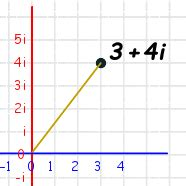
\includegraphics[scale = 0.5]{media/bspkomplexezahl.jpeg}
%     % \end{center}$
%     \begin{center}
%         \begin{tikzpicture}[scale=0.4]
%             % Gitter
%             \draw[dashed, very thin, gray] (-5,-5) grid (5,5);

%             % Achsen mit Skala
%             \draw[->] (-5,0) -- (5,0) node[right] {Reelle Achse};
%             \draw[->] (0,-5) -- (0,5) node[right] {Imaginäre Achse};
%             \foreach \x in {-4,-3,-2,-1,1,2,3,4} 
%                 \draw (\x,0) -- (\x,-0.2) node[below] {$\x$};
%              \foreach \y in {-4,-3,-2,2,3,4}
%                 \draw (0,\y) -- (-0.2,\y) node[left] {$\y i$};
%             \draw (0,1) -- (-0.2,1) node[left] {$i$};
%             %\draw (0,-1) -- (-0.2,-1) node[left] {$-i$};

%             % Punkte und Markierungen
%             %\draw[dashed, very thin, gray] (2,0) -- (2,3) -- (0,3);
%             \fill[red] (0,1) circle (0.1) node[right] {$z = i$};
%             \fill[purple] (2,3) circle (0.1) node[right] {$w = 2 + 3i$};
%         \end{tikzpicture}
%     \end{center}


% \end{definition}

% Die Gauss'sche Zahlenebene ermöglicht eine geometrische Deutung der Operationen mit komplexen Zahlen:

% \begin{satz}
%     {Geometrische Sicht auf die Addition von komplexen Zahlen}{}
%     Die Addition zweier komplexen Zahlen \(z = a + b \cdot i\) und \(w = x + y \cdot i\) entspricht der Addition der Ortsvektoren \(\vec{z} = \begin{pmatrix} a \\ b \end{pmatrix}\) und \(\vec{w} = \begin{pmatrix} x \\ y \end{pmatrix}\). Das Gleiche gilt für die Subtraktion.
%     % \begin{center}
%     %     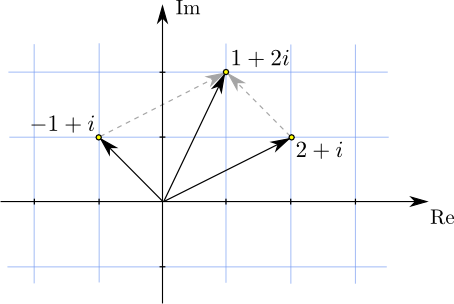
\includegraphics[width = 0.5 \textwidth]{media/additioninC.png}
%     % \end{center}
%     \begin{center}

%         Addition

%         \begin{tikzpicture}[scale = 1]


%             % Achsen mit Skala
%             \draw[->, thick] (-1.5,0) -- (4.5,0) node[above] {$\RE$};
%             \draw[->, thick] (0,-1.5) -- (0,2.5) node[right] {$\IM$};
%             \foreach \x in {-1,2,3,4} 
%                 \draw (\x,0.1) -- (\x,-0.1) ;
%             \foreach \y in {-1,2,} 
%                 \draw (0.1,\y) -- (-0.1,\y) ;
%             \draw (0.1,1) -- (-0.1,1) node[left] {$i$};
%             \draw (1,0.1) -- (1,-0.1) node[below] {$1$};

%              % Vektoren
%              \draw[->, thick, dashed] (0,0) -- node[above] {$\vec{z}_1$} ++(1,5/4) node[above left, ForestGreen] {$z_1 = a + bi$};
%              \draw[->, thick, dashed] (0,0) -- node[below right] {$\vec{z}_2$} ++(2,3/4) node[below right, ForestGreen] {$z_2 = c + di$};
%              \draw[->, thick, orange] (0,0) -- (3,2) node[above right, orange] {$z_1 + z_2$};
%              \draw[->, thick, dashed] (1,5/4) -- (3,2) ; 
%              \draw[->, thick, dashed] (2,3/4) -- (3,2) ; 

%              % Punkte
%              \fill[ForestGreen] (1,5/4) circle (0.05);
%              \fill[ForestGreen] (2,3/4) circle (0.05) ;
%              \fill[orange] (3,2) circle (0.05);
%         \end{tikzpicture}

%     \end{center}

% \end{satz}
% Zur geometrischen Deutung der Multiplikation benötigen wir eine andere Darstellung der komplexen Zahlen.
% \subsubsection{Die Polarform einer komplexen Zahl}
% Mit Ausnahme von 0 kann jeder Punkt der (Zahlen)Ebene eindeutig durch seinen Abstand zum Ursprung und dem Winkel zwischen dem entsprechenden Ortsvektor und der reellen Achse angegeben werden.
% \begin{definition}
%     {Polarform}{}
%     Die Polarform einer komplexen Zahl \(z = x + yi\) lautet \(z = r \operatorname{cis} \varphi\). Dabei ist \(r > 0\) der Abstand vom Ursprung und \(\varphi\) der Winkel zwischen dem Ortsvektor und der positiven x-Achse. Die Form \(z = x + yi\) nennt man die kartesische Form.
%     % \begin{center}
%     %     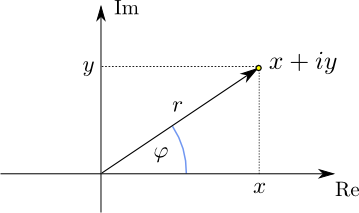
\includegraphics[scale = 0.5]{media/polarform.png}
%     % \end{center}
%     \begin{center}
%         \begin{tikzpicture}[scale = 0.7]
%             % Achsen mit Skala
%             \draw[->, thick] (-1.5,0) -- (4.5,0) node[above] {$\operatorname{Re}$};
%             \draw[->, thick] (0,-1.5) -- (0,2.5) node[right] {$\operatorname{Im}$};
%             \foreach \x in {-1,2,3,4} 
%                 \draw (\x,0.1) -- (\x,-0.1) ;
%             \foreach \y in {-1,2,} 
%                 \draw (0.1,\y) -- (-0.1,\y) ;
%             \draw (0.1,1) -- (-0.1,1) node[left] {$i$};
%             \draw (1,0.1) -- (1,-0.1) node[below] {$1$};

%             % Vektoren
%             \draw[->, thick] (0,0) -- node[above] {$r$}  ++(2.5, 2) ;

%             % Punkte
%             \fill[ForestGreen] (2.5,2) circle (0.05) node[above, ForestGreen] {$z$};

%             % Winkel
%             \draw[thick, ->] (1.2,0) arc (0:38:1.2) node[midway, right] {$\varphi$};

%         \end{tikzpicture}   
%     \end{center}

% \end{definition}
% Der folgende Satz erklärt, wie man die Polarform aus der kartesischen Form ermittelt und umgekehrt.


% \begin{satz}
%     {Umwandlung kartesische Form und Polarform}{}
%     Es gelten folgende Umrechnungsformeln für \(z = x + yi = r \operatorname{cis} (\varphi)\):


% \begin{align*}
% x &= r \cos \varphi \\
% y &= r \sin \varphi
% \end{align*}


% und

% \begin{align*}
% r &= |z| = \sqrt{x^2 + y^2} \\
% \varphi &= 
% \begin{cases}
% \arctan \left(\frac{y}{x}\right), & \text{falls } x > 0 \\
% \pi + \arctan \left(\frac{y}{x}\right), & \text{falls } x < 0
% \end{cases}
% \end{align*}


% \end{satz}

% \emph{Bemerkung:} $\operatorname{cis} (\varphi)$ ist eine Abkürzung für $\cos \varphi + i \sin \varphi$

% Komplexe Zahlen in Polarform lassen sich einfach multiplizieren:
% \begin{satz}
%     {Multiplikation in Polarform}{}
%     Sei \(z = r_1 \operatorname{cis} \varphi_1\), \(w = r_2 \operatorname{cis} \varphi_2\).
% Dann gilt:
% \[z \cdot w = r_1 r_2 \operatorname{cis} (\varphi_1 + \varphi_2)\]

% \[\frac{z}{w} = \frac{r_1}{r_2} \operatorname{cis} (\varphi_1 - \varphi_2)\]

% \[z^n = r_1^n \operatorname{cis}(n \varphi_1)\]
% % \begin{center}
% %     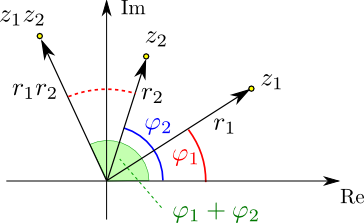
\includegraphics[scale = 0.5]{media/multiplikation-461714259.png}
% % \end{center}

% \begin{center}
%     \begin{tikzpicture}[scale = 1]
%         % Gitter
%         \draw[dashed, very thin, gray] (-4,-4) grid (4,4);

%         % Achsen mit Skala
%         \draw[->] (-4,0) -- (4,0) node[above] {$\RE$};
%         \draw[->] (0,-4) -- (0,4) node[right] {$\IM$};
%         \foreach \x in {-3,-2,-1,1,2,3} 
%             \draw (\x,0) -- (\x,-0.2) ;
%          \foreach \y in {-3,-2, -1,2,3}
%             \draw (0,\y) -- (-0.2,\y) ;
%         \draw (0,1) -- (-0.2,1) node[left] {$i$};
%         \draw (1,0) -- (1,-0.2) node[below] {$1$};


%         % Punkt z1
%         \coordinate (z1) at (60:1.5);
%         \fill[ForestGreen] (z1) circle (0.05) node[above, ForestGreen] {$z_1$};
%         \draw[ForestGreen](0,0) -- (z1);
%         \draw[thick, ->, ForestGreen] (1, 0) arc (0:60:1) node[midway, left] {$\varphi_1$};

%          % Punkt z
%          \coordinate (z) at (130:2);
%          \fill[blue] (z) circle (0.05) node[above, blue] {$z$};
%          \draw[blue](0,0) -- (z);
%          \draw[thick, ->, blue] (1.2, 0) arc (0:130:1.2) node[midway, above left] {$\varphi$};
%          \draw[dashed] (0,0) circle (2);

%          % Punkt z_1*z
%          \coordinate (z1z) at (190:3);
%          \fill[red] (z1z) circle (0.05) node[below, red] {$z_1\cdot z$};
%          \draw[red](0,0) -- (z1z);
%          \draw[thick, ->, red] (130:1.2) arc (130:190:1.2) node[midway, left] {$\varphi_1$};


%     \end{tikzpicture}   
% \end{center}


% \end{satz}
% \begin{bsp}
%     {Rein kubische Gleichung}{}
%     Die Gleichung \(z^3 = -27\) hat in \(\mathbb{C}\) drei Lösungen. Diese findet man am einfachsten, indem man die Polarform verwendet. Sei \(z = r \operatorname{cis}(\varphi)\). Dann ist \(z^3 = r^3 \operatorname{cis}(3\varphi)\). Weiter ist \(-27 = 27 \operatorname{cis}(\pi)\). Also gilt
% \[r^3 \operatorname{cis}(3\varphi) = 27 \operatorname{cis}(\pi)\]

% Daraus folgt
% \[
% \begin{cases}
%     r^3 = 27 \\
%     3\varphi \equiv \pi \pmod{2\pi}
% \end{cases}
% \]

% Daraus ergibt sich
% \[r = 3 \quad \text{und} \quad \varphi = \frac{\pi}{3} \text{ oder } \pi \text{ oder } \frac{5\pi}{3}\]

% Die Lösungen lauten also
% \[z_1 = 3 \operatorname{cis}\left(\frac{\pi}{3}\right), \quad z_2 = 3 \operatorname{cis}(\pi) = -3, \quad z_3 = 3 \operatorname{cis}\left(\frac{5\pi}{3}\right)\]


% \end{bsp}



% \clearpage
%\subsection{Die Exponentialfunktion auf \texorpdfstring{$\C$}{C}}


\clearpage
Mit komplexen Zahlen kann man die vier Grundoperationen ausführen und in den vergangenen Kapitel haben wir gelernt, wie man einige Funktionen wie Sinus, Cosinus und die Funktion $f(x)=e^x$ genau mit diesen vier Grundoperationen berechnen kann. Damit lassen sich diese Funktionen so erweitern, dass auch komplexe Zahlen als Inputs möglich sind!

\begin{definition}
	{}{Die Exponentialfunktion für komplexe Argumente}
	Für \(z \in \mathbb{C}\) sei
	\[e^z = \sum_{k=0}^{\infty} \frac{z^k}{k!} = 1 + \frac{z}{1!} + \frac{z^2}{2!} + \ldots\]

\end{definition}

\begin{bsp}
	{$e^i$}{}
	\[e^i = 1 + \frac{i}{1!} + \frac{i^2}{2!} + \frac{i^3}{3!} + \frac{i^4}{4!} + \frac{i^5}{5!} + \ldots
		%= 1 + i - \frac{1}{2} - \frac{i}{6} + \frac{1}{24} + \frac{i}{120} - \ldots 
		\approx 0.54 + 0.84i\]

\end{bsp}
Der Schweizer Mathematiker Leonhard Euler (1707-1783) gehört zu den bedeutendsten Persönlichkeiten in der Geschichte der Mathematik. In seinem Werk \textit{Introductio in analysin infinitorum}, das 1748 erschienen ist, beweist er die sogenannte Eulersche Formel, die einen Zusammenhang zwischen der komplexen Exponentialfunktion und den trigonometrischen Funktionen herstellt. Eine Folgerung davon ist die berühmte Eulersche Identität, welche eine wahrhaft erstaunliche Beziehung zwischen den fünf wichtigsten Zahlen aufdeckt.


\begin{figure}[h]
	\begin{center}
		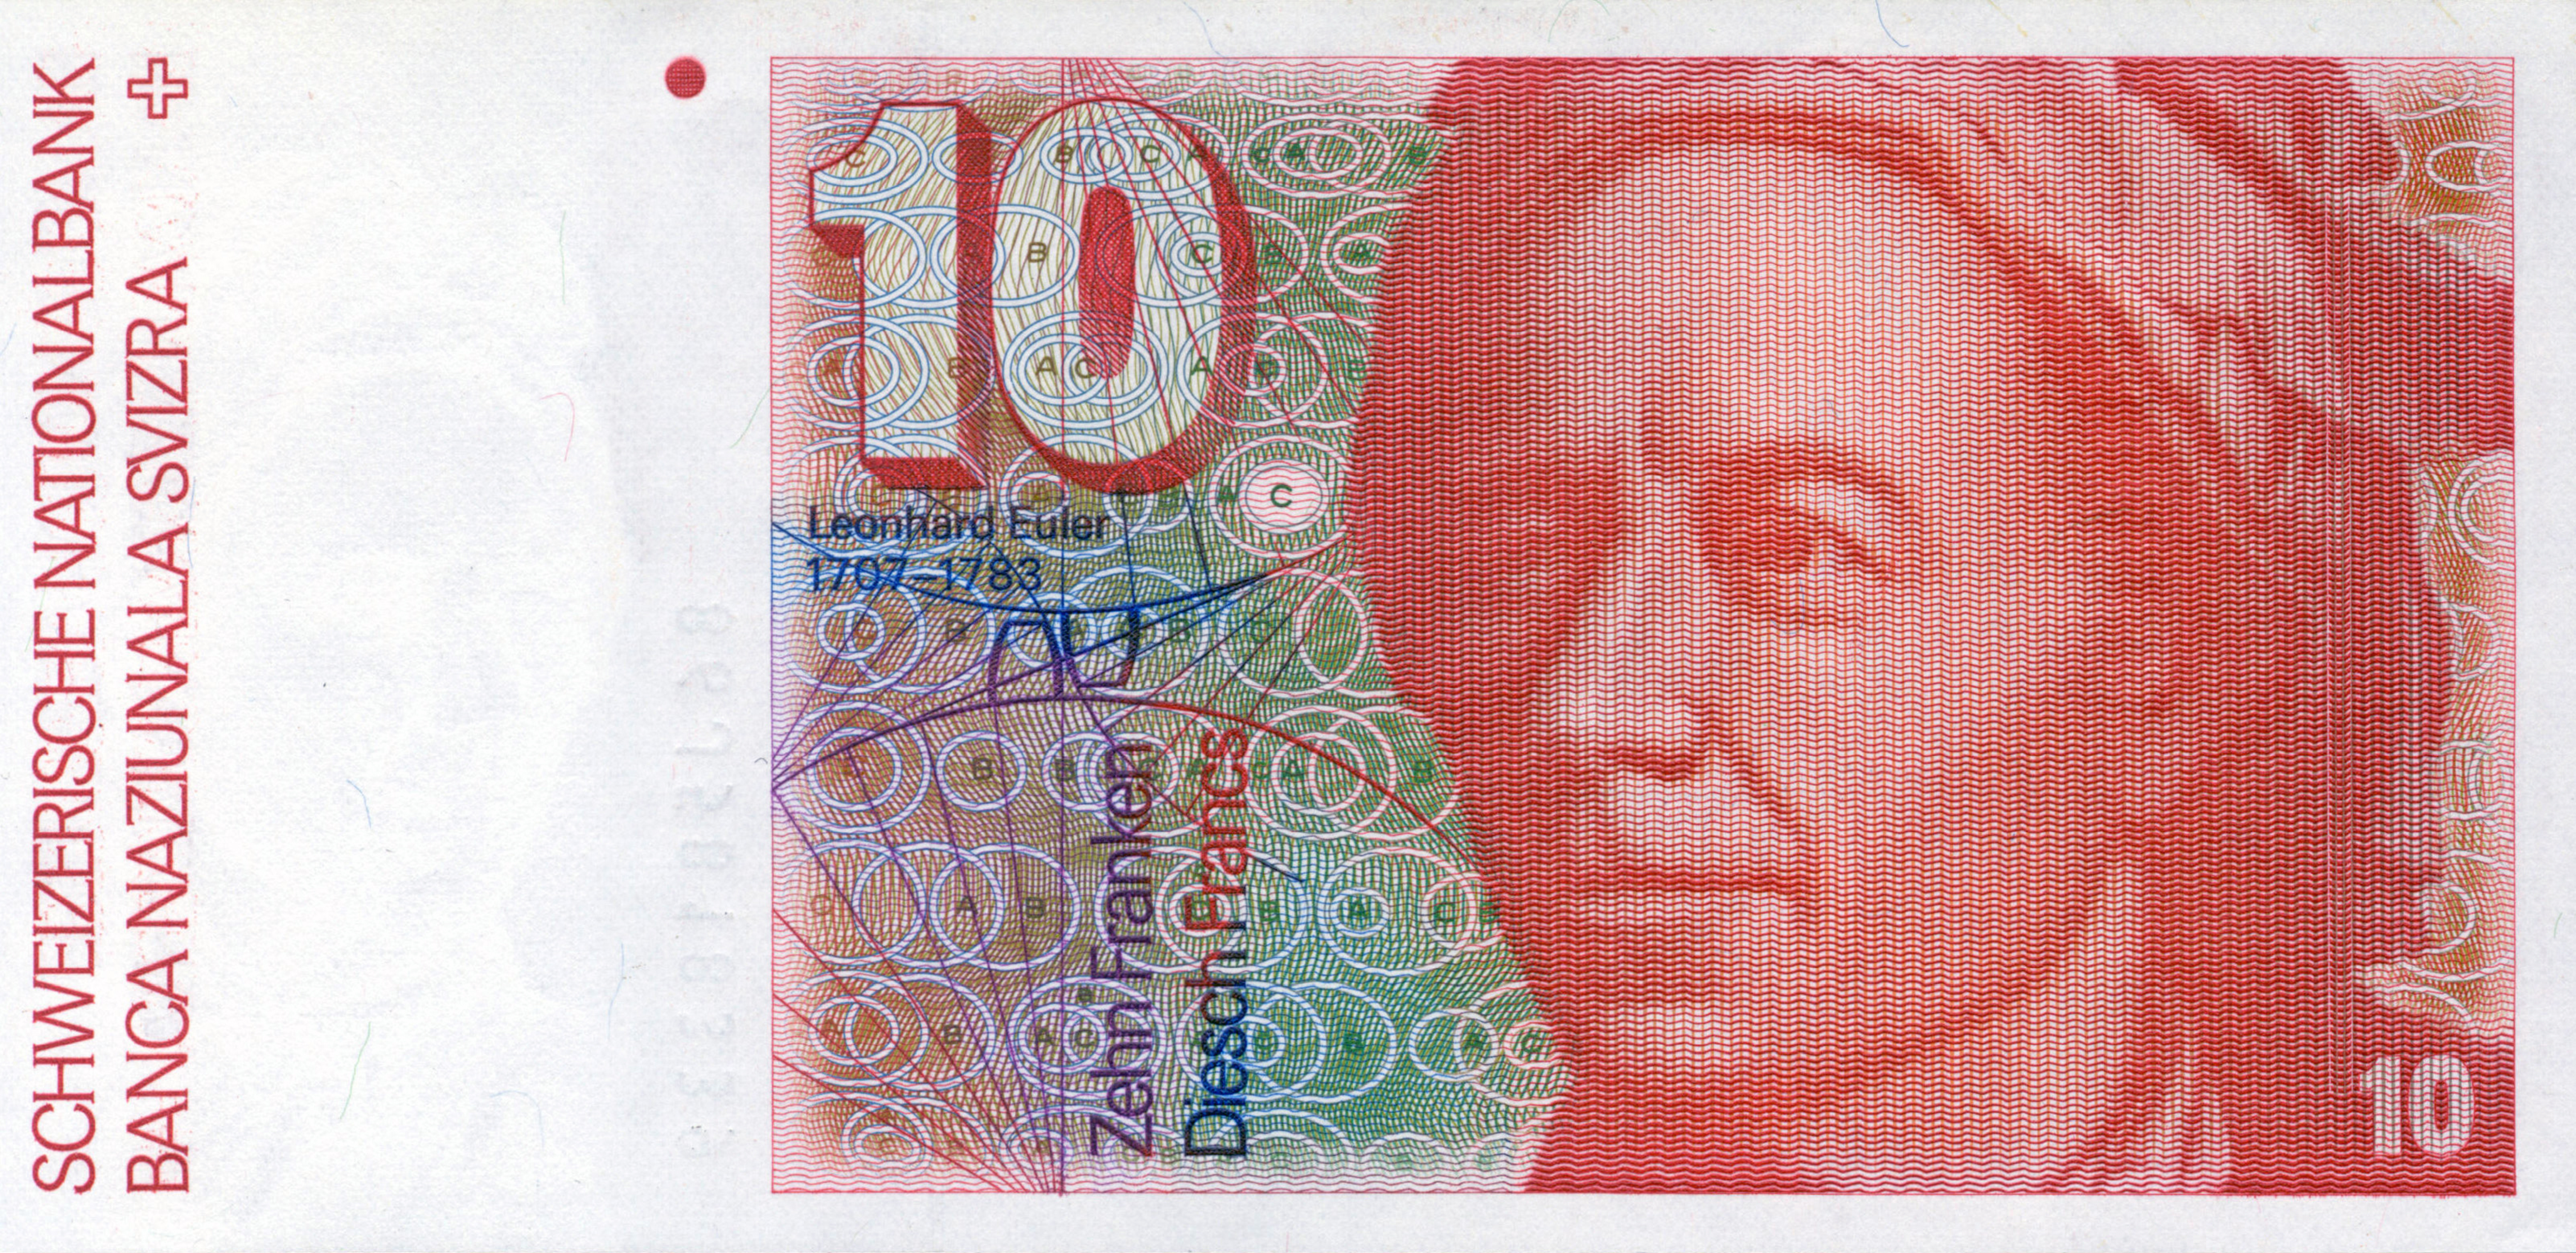
\includegraphics[width = 0.6 \textwidth]{media/Euler-10_Swiss_Franc_banknote_(front).pdf}
		\caption{Schweizer 10-Franken-Note bis 1995}
	\end{center}
\end{figure}



\begin{LA}
	{Entdecken Sie die Eulersche Formel und die Eulersche Identität}{}
	\begin{enumerate}
		\item Berechnen Sie eine Näherung für \(e^{i \pi / 2}\), indem Sie die ersten 6 Summanden der Summe in der Definition berechnen. (Kontrolle: \(e^{i \pi / 2}\approx 0.0200 + 1.0045 i \))
		\item  Sei \(x \in \mathbb{R}\). Stellen Sie die Summe für die Zahl \(e^{i \cdot x}\) auf und vereinfachen Sie den Real- und Imaginärteil. Am Schluss sollten Sie ein schönes Resultat erhalten: Die Eulersche Formel!
		\item   Bestimmen Sie mit der Formel aus 2. die Zahl \(e^{i \pi}\).
	\end{enumerate}



\end{LA}

\clearpage
\begin{satz}
	{Eulersche Identität und Eulersche Formel}{}
	Sei \(\varphi \in \mathbb{R}\). Dann gilt
	\[e^{i \cdot \varphi} =\phantom{\cos(\varphi) + i \cdot \sin (\varphi)}\]
	% \begin{center}
	%     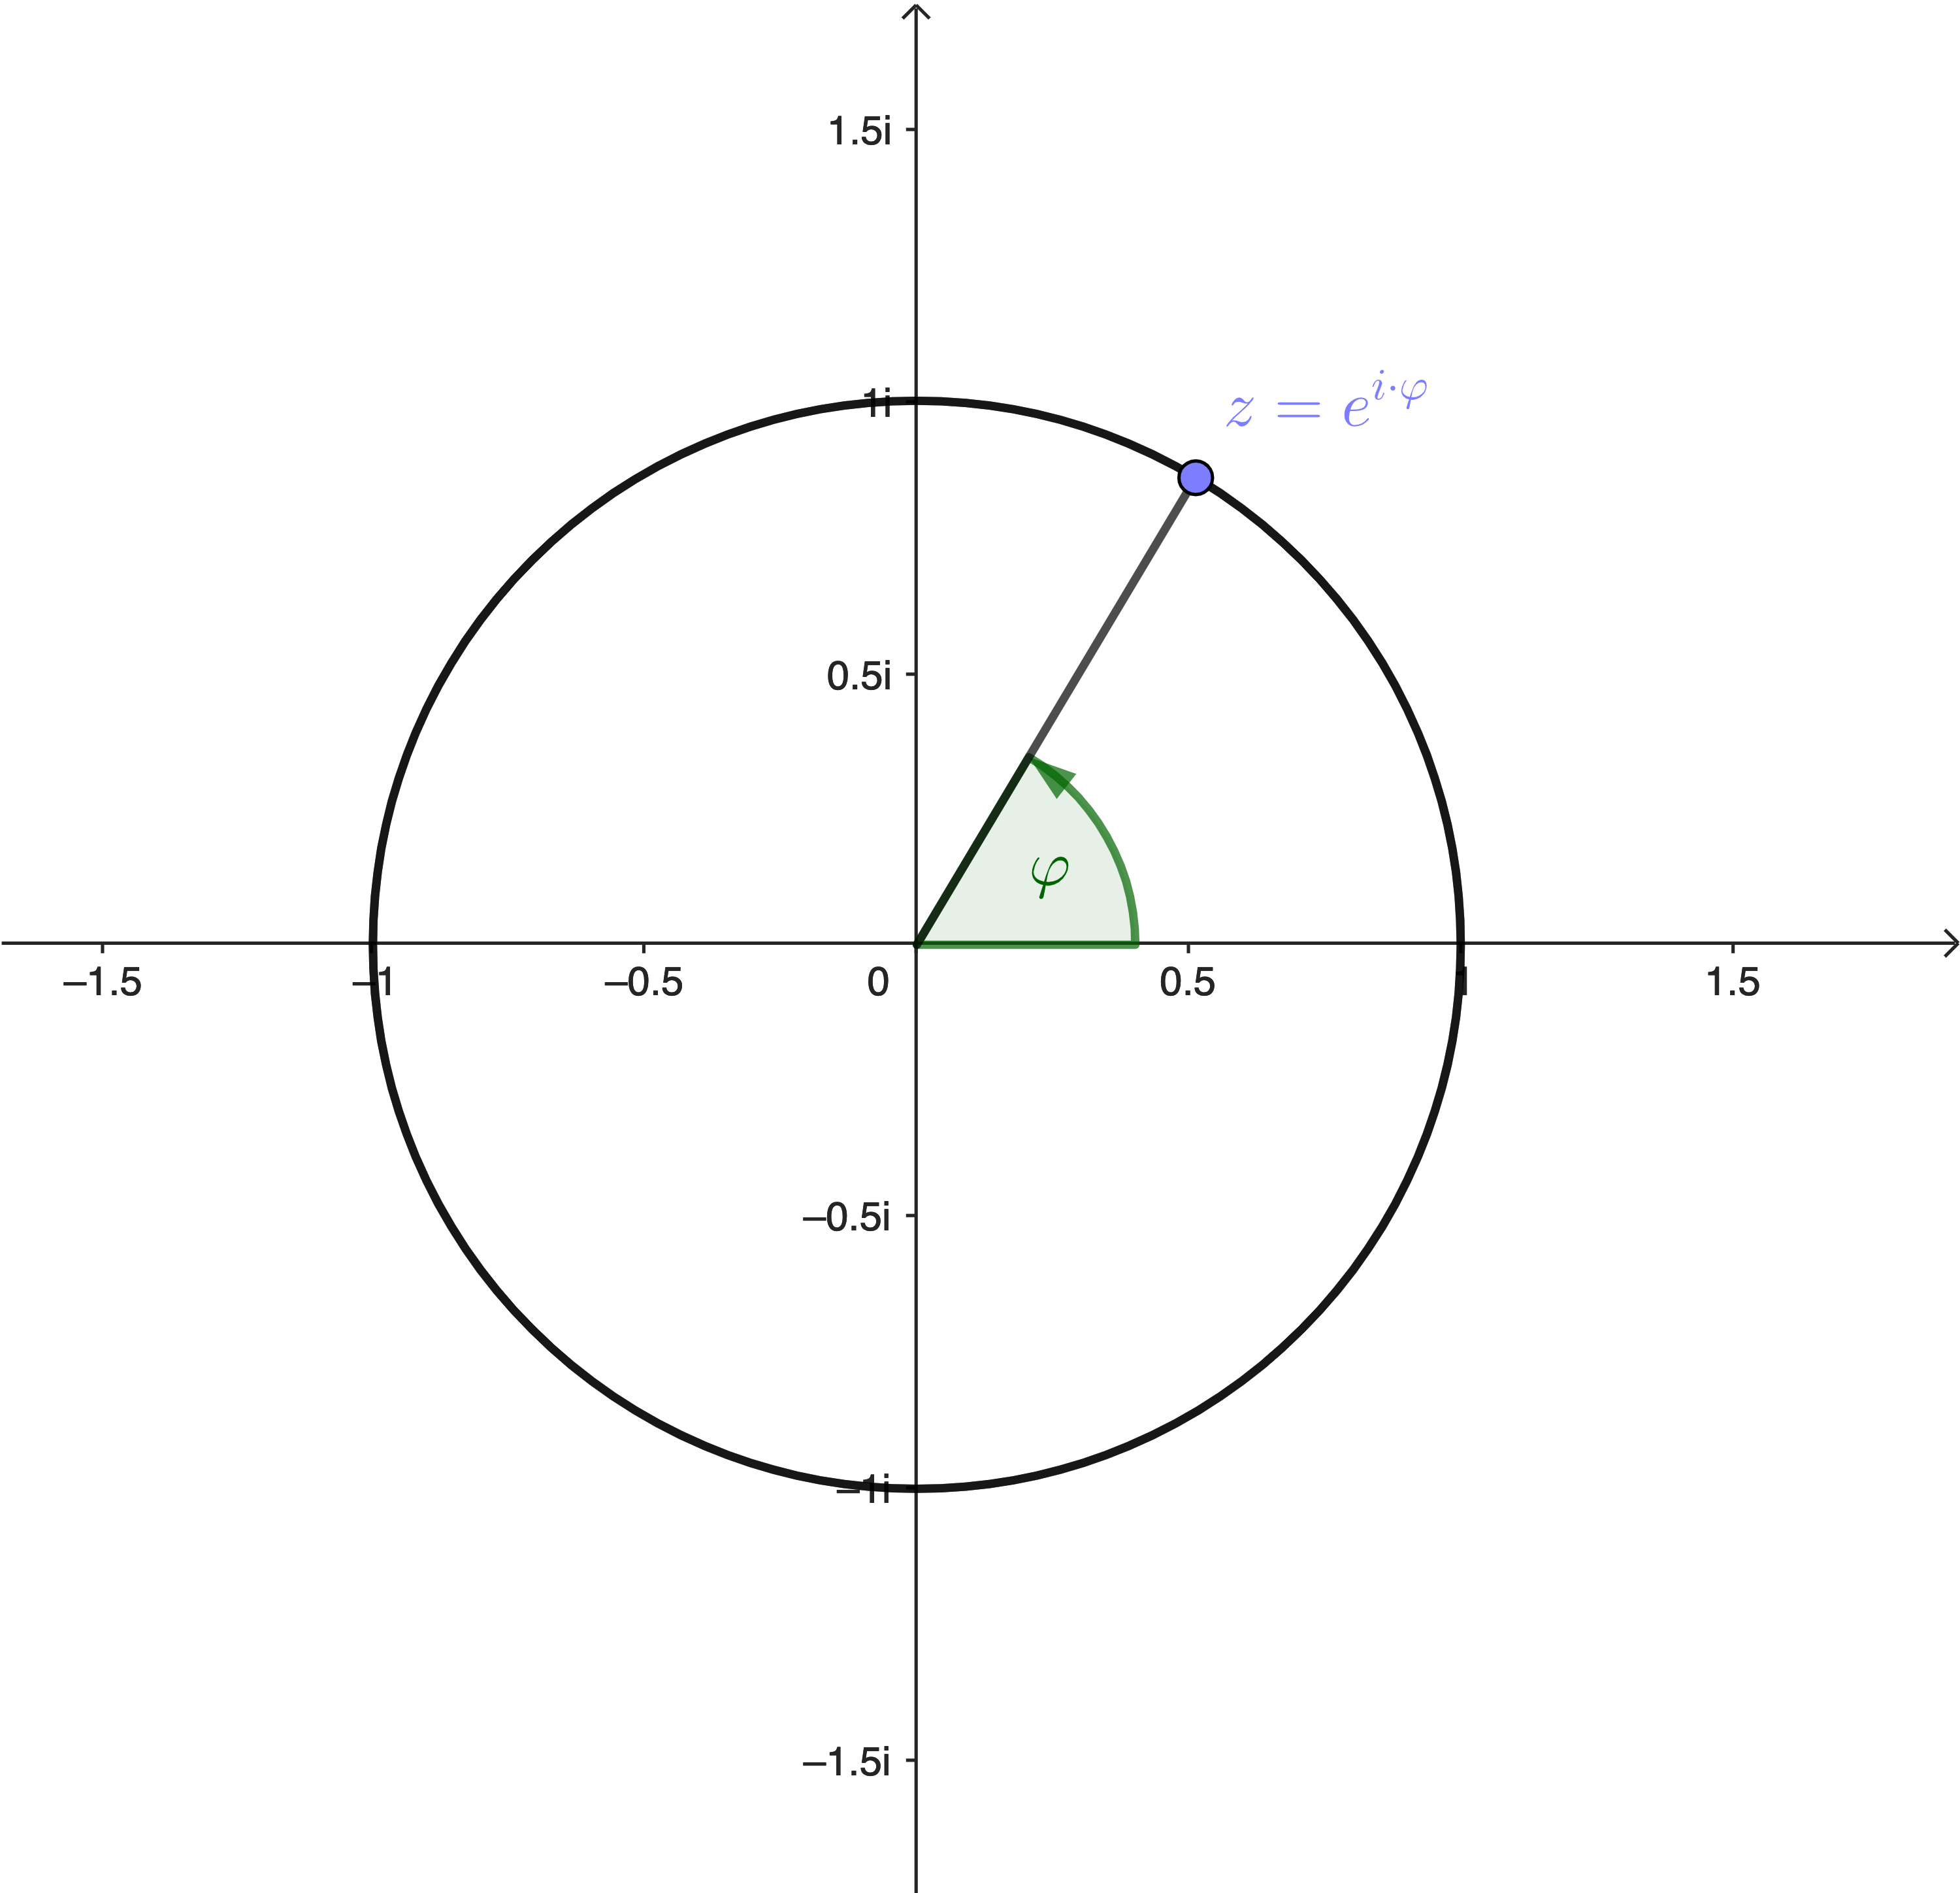
\includegraphics[width = 0.5 \textwidth]{media/eulerformel.png}
	% \end{center}


	\begin{center}
		\begin{tikzpicture}[scale = 1.5]
			% Gitter
			\draw[dashed, very thin, gray] (-2,-2) grid (2,2);

			% Achsen mit Skala
			\draw[->] (-2,0) -- (2,0) node[above] {$\RE$};
			\draw[->] (0,-2) -- (0,2) node[right] {$\IM$};
			\foreach \x in {-1,1}
			\draw (\x,0) -- (\x,-0.2) ;
			\foreach \y in {-1}
			\draw (0,\y) -- (-0.2,\y) ;
			\draw (0,1) -- (-0.2,1) node[above left] {$i$};
			\draw (1,0) -- (1,-0.2) node[below right] {$1$};



			% Einheitskreis
			\draw[dashed] (0,0) circle (1);
			% Punkt z
			\coordinate (z) at (40:1);
			\fill[blue] (z) circle (0.05) node[above right, blue] {$e^{i \cdot \varphi}$};
			\draw[orange](0,0) -- (z);
			\draw[thick, ->, red] (0.5, 0) arc (0:40:0.5) node[midway, right] {$\varphi$};


			%  % Punkt z^2
			%  \coordinate (z2) at (80:1);
			%  \fill[blue] (z2) circle (0.05) node[above right, blue] {$z^2$};
			%  \draw[orange](0,0) -- (z2);
			%  \draw[thick, ->, red] (40:0.5) arc (40:80:0.5) node[midway, above right] {$\varphi$};

			%   % Punkt z^3
			%   \coordinate (z3) at (120:1);
			%   \fill[blue] (z3) circle (0.05) node[above left, blue] {$z^3$};
			%   \draw[orange](0,0) -- (z3);
			%   \draw[thick, ->, red] (80:0.5) arc (80:120:0.5) node[midway, above] {$\varphi$};

		\end{tikzpicture}
	\end{center}
	Im Spezialfall \(\varphi = \pi\)   erhält man die berühmte eulersche Identität:

	\vspace{2 cm}
\end{satz}



\emph{Bemerkungen:}
\begin{itemize}
	\item Die Eulersche Identität vereinigt die „fünf wichtigsten Zahlen des Universums“ in einer einfachen Gleichung. Das Erstaunliche ist, dass diese fünf Zahlen aus ganz verschiedenen Gebieten der Mathematik stammen:
	      \begin{itemize}
		      \item $e$ spielt eine wichtige Rolle in der Differenzialrechnung
		      \item $i$ ist die imaginäre Einheit
		      \item $\pi$ ist die Kreiszahl
		      \item $1$ ist das neutrale Element der Multiplikation
		      \item $0$ ist das neutrale Element der Addition.
	      \end{itemize}
	\item Der Winkel \( \varphi \) ist im Bogenmass.
	\item In Zukunft schreiben wir nicht mehr \( z = r \cdot \text{cis} (\varphi) \), sondern \( z = r\cdot e^{i\varphi} \).
	\item Die Potenzgesetze gelten auch für komplexe Exponenten. Insbesondere gelten die Formeln von De Moivre:
	      \[ e^{i\varphi} \cdot e^{i\psi} = \text{cis}(\varphi) \cdot \text{cis}(\psi) = \text{cis}(\varphi+\psi) = e^{i(\varphi+\psi)} \]
	      \[ (e^{i\varphi})^k = e^{i \cdot k\varphi} \]
\end{itemize}




\clearpage
\begin{ueb}
	{}{}
	\begin{enumerate}
		\item Berechnen Sie den Realteil $\operatorname{Re}(e^{x+iy})$, wobei $x, y \in \mathbb{R}$. Verwenden Sie: $e^{x+iy} = e^x \cdot e^{iy}$.

		\item Berechnen Sie $|e^{i(x+iy)}|$.

		\item Geben Sie eine Lösung der Gleichung $e^z = -2i$ an. Finden Sie auch eine zweite?

		\item Zeigen Sie, dass die Exponentialfunktion $2\pi i$-periodisch ist, das heisst: Für alle $z \in \mathbb{C}$ gilt $e^{z+2\pi i} = e^z$.

		\item Was ist das Bild der folgenden Mengen unter der Exponentialfunktion?
		      \begin{enumerate}
			      \item Imaginäre Achse: $\operatorname{Re}(z) = 0$
			      \item Reelle Achse: $\operatorname{Im}(z) = 0$
			      \item $\operatorname{Re}(z) = 2$
			      \item $\operatorname{Im}(z) = 2$
		      \end{enumerate}
		\item Zur Erinnerung: Die Funktionen Cosinus hyperbolicus und Sinus hyperbolicus sind definiert als:
		      $$ \cosh(x) = \frac{e^x+e^{-x}}{2} \qquad \sinh(x) = \frac{e^x-e^{-x}}{2} $$
		      und es gilt, dass $\cosh'(x) = \sinh(x)$ und $\sinh'(x) = \cosh(x)$.

		      Verwenden Sie die Reihendarstellung von $\sin$ und $\cos$ und die Taylorentwicklung um die Stelle $x_0 = 0$ der Funktionen $\cosh$ und $\sinh$, um zu zeigen, dass für $x\in\R$ gilt:
		      $$\cos(ix) = \cosh(x)\quad\text{und} \quad \frac{\sin(ix)}{i} = \sinh(x)$$

		      %   \begin{enumerate}
		      %       \item Zeigen Sie, dass $\cosh^2(x) - \sinh^2(x) = 1$ ist.
		      %       \item Berechnen Sie die Ableitungen von $\cosh(x)$ und $\sinh(x)$ mit der Kettenregel.

		      %       \item Verwenden Sie die Reihendarstellung von $\sin$ und $\cos$ und die Taylorentwicklung um die Stelle $x_0 = 0$ der Funktionen $\cosh$ und $\sinh$, um zu zeigen, dass für $x\in\R$ gilt:
		      %             $$\cos(ix) = \cosh(x)\quad\text{und} \quad \frac{\sin(ix)}{i} = \sinh(x)$$
		      %   \end{enumerate}
	\end{enumerate}
\end{ueb}

\clearpage
\emph{Lösungen}
\begin{enumerate}
	\item $\operatorname{Re}(e^{x+iy}) = e^x \cos y$
	\item $|e^{i(x+iy)}| = e^{-y}$
	\item $z = \ln(2) + \frac{3\pi}{2} i$. Ausserdem alle Zahlen der Form $z = \ln(2) + \left(\frac{3\pi}{2}+2k\pi\right) i$. Aus diesem Grund gibt es keinen Logarithmus für komplexe Zahlen.
	\item $e^{z+2\pi i} = e^z\cdot e^{2\pi i} = e^z\cdot 1 = e^z$
	\item Bildmengen:
	      \begin{enumerate}
		      \item Einheitskreis
		      \item Positive reelle Achse
		      \item Kreis um den Ursprung mit Radius $e^2$
		      \item Halbgerade $\{t\cdot e ^{2i} | t \in \R^+\}$
	      \end{enumerate}
	\item Die Taylorentwicklung von $\cosh$ lautet:
	      $$\cosh(x) = 1+\frac{x^2}{2!}+\frac{x^4}{4!}+\frac{x^6}{6!} +\dots  $$
	      Wenn man $ix$ in die Reihendarstellung von $\cos$ einsetzt, erhält man:
	      \begin{align*}
		      \cos(ix) & = 1-\frac{(ix)^2}{2!}+\frac{(ix)^4}{4!}-\frac{(ix)^6}{6!} +\dots \\
		               & = 1+\frac{x^2}{2!}+\frac{x^4}{4!}+\frac{x^6}{6!} +\dots          \\
		               & = \cosh(x)
	      \end{align*}
	      Analog für $\sinh$

	      % Cosh und Sinh:
	      %       \begin{enumerate}

	      % 	      \item \begin{align*}
	      % 		            \cosh^2(x) - \sinh^2(x) & =\left(\frac{e^x+e^{-x}}{2}\right)^2 - \left(\frac{e^x-e^{-x}}{2}\right)^2 \\
	      % 		                                    & = \frac{e^{2x} +2 + e^{-2x}}{4} - \frac{e^{2x} - 2 + e^{-2x}}{4}           \\
	      % 		                                    & = \frac{4}{4}                                                              \\
	      % 		                                    & = 1
	      % 	            \end{align*}
	      % 	      \item $(\cosh(x))' = \sinh(x), \quad (\sinh(x))' = \cosh(x)$
	      % 	      \item Die Taylorentwicklung von $\cosh$ lautet:
	      % 	            $$\cosh(x) = 1+\frac{x^2}{2!}+\frac{x^4}{4!}+\frac{x^6}{6!} +\dots  $$
	      % 	            Wenn man $ix$ in die Reihendarstellung von $\sin$ einsetzt, erhält man:
	      % 	            \begin{align*}
	      % 		            \cos(ix) & = 1-\frac{(ix)^2}{2!}+\frac{(ix)^4}{4!}-\frac{(ix)^6}{6!} +\dots \\
	      % 		                     & = 1+\frac{x^2}{2!}+\frac{x^4}{4!}+\frac{x^6}{6!} +\dots          \\
	      % 		                     & = \cosh(x)
	      % 	            \end{align*}
	      % 	            Analog für $\sinh$
	      %   \end{enumerate}
\end{enumerate}




\clearpage
\subsection*{Additum: Matrixexponential}
Die Erweiterung der Exponentialfunktion auf komplexe Argumente (letztes Kapitel) wird die Behandlung von Differentialgleichungen vereinfachen. Bei Systemen von mehreren Differentialgleichungen wird es nützlich sein, Matrizen als Inputs der Exponentialfunktion in Betracht zu ziehen.
\begin{definition}
	{Matrixexponential}{}
	Für eine quadratische Matrix $A$ sei
	$$e^A = \sum_{k=0}^\infty \frac{A^k}{k!} = E + \frac{A}{1!} + \frac{A^2}{2!} + \dots $$
	Wobei $E$ die Einheitsmatrix ist.
\end{definition}
\begin{bsp}
	{Matrixexponential einer nilpotenten Matrix}{}
	Betrachten Sie die Matrix $N$:

	$$
		N = \begin{pmatrix}
			0 & 1 & 0 \\
			0 & 0 & 1 \\
			0 & 0 & 0 \\
		\end{pmatrix}
	$$

	Es gilt
	$$
		N^2 = \begin{pmatrix}
			0 & 0 & 1 \\
			0 & 0 & 0 \\
			0 & 0 & 0 \\
		\end{pmatrix},
		\qquad
		N^3 = \begin{pmatrix}
			0 & 0 & 0 \\
			0 & 0 & 0 \\
			0 & 0 & 0 \\
		\end{pmatrix}
	$$

	Für alle weiteren Potenzen der Matrix gilt dann $N^k=0, \, k\ge3$. Solche Matrizen nennt man \emph{nilpotent}. Die Matrixexponentialfunktion für diese Matrix kann dann wie folgt geschrieben werden:

	$$
		e^N = E + \frac{N}{1!} + \frac{N^2}{2!} = \begin{pmatrix}
			1 & 1 & \frac{1}{2} \\
			0 & 1 & 1           \\
			0 & 0 & 1           \\
		\end{pmatrix}
	$$


\end{bsp}

\begin{bsp}
	{Matrixexponential einer Diagonalmatrix}{eHochDiagonalmatrix}
	Betrachten Sie die Diagonalmatrix $D$:

	$$
		D = \begin{pmatrix}
			1 & 0 \\
			0 & 2 \\
		\end{pmatrix}
	$$

	Dann gilt
	$$ D^k = \begin{pmatrix}
			1 & 0   \\
			0 & 2^k \\
		\end{pmatrix}
	$$

	Das Matrixexponential $e^D$ für diese Matrix kann direkt berechnet werden:

	$$
		e^D = \sum_{k=0}^{\infty} \frac{D^k}{k!} = \begin{pmatrix}
			1 & 0 \\
			0 & 1 \\
		\end{pmatrix} + \frac{\begin{pmatrix}
				1 & 0 \\
				0 & 2 \\
			\end{pmatrix}}{1!} + \frac{\begin{pmatrix}
				1 & 0   \\
				0 & 2^2 \\
			\end{pmatrix}}{2!} + \frac{\begin{pmatrix}
				1 & 0   \\
				0 & 2^3 \\
			\end{pmatrix}}{3!} + \ldots
	$$

	Die Einträge der Matrix $e^D$ lauten dann:
	$$
		e^D = \begin{pmatrix}
			\sum_{k=0}^{\infty} \frac{1}{k!} & 0                                  \\
			0                                & \sum_{k=0}^{\infty} \frac{2^k}{k!}
		\end{pmatrix}
		= \begin{pmatrix}
			e^1 & 0   \\
			0   & e^2 \\
		\end{pmatrix}
	$$
	Wobei im letzten Schritt die Taylorreihe $e^x = \sum_{k=0}^{\infty} \frac{x^k}{k!}$ für $x=1$ und $x=2$ verwendet wurde.
\end{bsp}

\begin{bsp}{Matrixexponential einer diagonalisierbaren Matrix}{}
	Betrachten Sie die  Matrix $A$:

	$$
		A = \begin{pmatrix}
			2 & -1 \\
			0 & 3  \\
		\end{pmatrix}
	$$

	Um die Matrix $e^A$ zu bestimmen, müssen wir $A$ zuerst diagonalisieren. Wie man leicht nachrechnet, hat $A$ die Eigenwerte $\lambda_1 = 2$ und $\lambda_2 = 3$ mit den dazugehörigen Eigenvektoren $\vec{v}_1 = \begin{pmatrix}
			1 \\ 0
		\end{pmatrix}$ und $\vec{v}_2 = \begin{pmatrix}
			-1 \\ 1
		\end{pmatrix}$. Damit gilt
	$$
		A = TDT^{-1} = \begin{pmatrix}
			1 & -1 \\
			0 & 1  \\
		\end{pmatrix} \cdot
		\begin{pmatrix}
			2 & 0 \\
			0 & 3 \\
		\end{pmatrix} \cdot
		\begin{pmatrix}
			1 & -1 \\
			0 & 1  \\
		\end{pmatrix}^{-1}
	$$

	Für $A^2$ gilt dann $A^2 = TD\underbrace{T^{-1} T}_{E} DT^{-1} = TD^2T^{-1}$. Oder allgemein:
	%Damit lassen sich die Potenzen von $A$ leicht berechnen:
	$$
		A^k =TD^kT^{-1}=
		\begin{pmatrix}
			1 & -1 \\
			0 & 1  \\
		\end{pmatrix} \cdot
		\begin{pmatrix}
			2 & 0 \\
			0 & 3 \\
		\end{pmatrix}^k \cdot
		\begin{pmatrix}
			1 & -1 \\
			0 & 1  \\
		\end{pmatrix}^{-1}
	$$

	Für das Matrixexponential gilt nun:

	\begin{align*}
		e^A & = E + \frac{A}{1!} + \frac{A^2}{2!} + \dots                      \\
		    & = TET^{-1} + \frac{TDT^{-1}}{1!} + \frac{TD^2T^{-1}}{2!} + \dots \\
		    & = T\left(E + \frac{D}{1!} + \frac{D^2}{2!} + \dots\right) T^{-1} \\
		    & = T e^D T^{-1}
	\end{align*}
	Das Matrixexponential $e^D$ lässt sich nun leicht wie im Beispiel \ref*{bsp:eHochDiagonalmatrix} berechnen und man erhält schliesslich
	$$
		e^A = T e^D T^{-1} = \begin{pmatrix}
			1 & -1 \\
			0 & 1  \\
		\end{pmatrix} \cdot
		\begin{pmatrix}
			e^2 & 0   \\
			0   & e^3 \\
		\end{pmatrix}\cdot
		\begin{pmatrix}
			1 & -1 \\
			0 & 1  \\
		\end{pmatrix}^{-1} = \begin{pmatrix}
			e^2 & e^2-e^3 \\
			0   & e^3
		\end{pmatrix}
	$$

\end{bsp}
\clearpage
\begin{ueb}
	{}{}
	\begin{enumerate}
		\item Gegeben sei die  $2 \times 2$-Matrix $N$:
		      \[
			      N = \begin{pmatrix} 0 & 0 \\ 4 & 0 \end{pmatrix}
		      \]

		      Berechnen Sie $e^N$.
		\item Gegeben sei die  $3 \times 3$-Matrix $D$:
		      \[
			      D = \begin{pmatrix} 3 & 0 & 0 \\ 0 & -1 & 0 \\ 0& 0 & 0 \end{pmatrix}
		      \]

		      Berechnen Sie $e^D$.
		\item Gegeben sei die  $2 \times 2$-Matrix $A$:
		      \[
			      A = \begin{pmatrix}
				      5  & -2 \\
				      12 & -5
			      \end{pmatrix}
		      \]
		      Berechnen Sie $e^A$.
		\item \emph{Challenge}: Sei $x\in\R$ und $$M = \begin{pmatrix}
				      0 & x \\-x & 0
			      \end{pmatrix}$$
		      Berechnen Sie $e^M$.

		      Tipp: Berechnen Sie einige Matrixpotenten $M^k$ für $k = 1, 2, 3, 4, 5, \dots$ und versuchen Sie, darin ein Muster zu finden.



	\end{enumerate}
\end{ueb}
\clearpage
\emph{Lösungen}
\begin{enumerate}
	\item Da $N^2 = 0$, folgt:

	      \[
		      e^N = E + N + \frac{N^2}{2!} + \frac{N^3}{3!} + \ldots = E + N
	      \]

	      Setzen wir die Werte ein:

	      \[
		      e^N = \begin{pmatrix} 1 & 0 \\ 0 & 1 \end{pmatrix} + \begin{pmatrix} 0 & 0 \\ 4 & 0 \end{pmatrix} = \begin{pmatrix} 1 & 0 \\ 4 & 1 \end{pmatrix}
	      \]

	      Daher ist die Lösung $e^N = \begin{pmatrix} 1 & 0 \\ 4 & 1 \end{pmatrix}$.
	\item $D$ ist eine Diagonalmatrix. Also
	      $$
		      e^D = \begin{pmatrix} e^3 & 0 & 0 \\ 0 & e^{-1} & 0 \\ 0& 0 & e^0 \end{pmatrix} = \begin{pmatrix} e^3 & 0 & 0 \\ 0 & 1/e & 0 \\ 0& 0 & 1 \end{pmatrix}
	      $$
	\item $$ e^A = T e^D T^{-1} = \begin{pmatrix}
			      1 & 1 \\
			      3 & 2 \\
		      \end{pmatrix} \cdot
		      \begin{pmatrix}
			      e^{-1} & 0     \\
			      0      & e^{1} \\
		      \end{pmatrix}\cdot
		      \begin{pmatrix}
			      1 & 1 \\
			      3 & 2 \\
		      \end{pmatrix}^{-1} = \begin{pmatrix}
			      -\frac{2}{e}+3e & \frac{e}{e}-e  \\
			      -\frac{6}{e}+6e & \frac{3}{e}-2e
		      \end{pmatrix}
	      $$
	\item Für die Potenzen $M^0$, $M^1$, $M^{2}$, $M^{3}$, $M^{4}$ und $M^{5}$ erhält man:
	      \begin{align*}
		      M^0 & =  \begin{pmatrix} x^{0} &  0\\ 0 & x^{0} \end{pmatrix}  \\
		      M^1 & = \begin{pmatrix} 0 & x^{1} \\ -x^{1} & 0 \end{pmatrix}  \\
		      M^2 & = \begin{pmatrix}  -x^{2} & 0 \\ 0& -x^{2} \end{pmatrix} \\
		      M^3 & = \begin{pmatrix} 0 & -x^{3} \\ x^{3} & 0 \end{pmatrix}  \\
		      M^4 & = \begin{pmatrix} x^{4} &  0\\ 0 & x^{4} \end{pmatrix}
	      \end{align*}
	      Diese Muster setzt sich so weiter fort. Für jedes $k\in\N$ gilt:
	      \begin{align*}
		      M^{4k}   & = \begin{pmatrix} x^{4k} &  0\\ 0 & x^{4k} \end{pmatrix},       \\
		      M^{4k+1} & = \begin{pmatrix} 0 & x^{4k+1} \\ -x^{4k+1} & 0 \end{pmatrix},  \\
		      M^{4k+2} & = \begin{pmatrix}  -x^{4k+2} & 0 \\ 0& -x^{4k+2} \end{pmatrix}, \\
		      M^{4k+3} & = \begin{pmatrix} 0 & -x^{4k+3} \\ x^{4k+3} & 0 \end{pmatrix}.
	      \end{align*}
	      Damit folgt
	      $$ e^M = \begin{pmatrix}
			      \sum_{k=0}^\infty (-1)^k \frac{x^{2k}}{(2k)!}      & \sum_{k=0}^\infty (-1)^k \frac{x^{2k+1}}{(2k+1)!} \\
			      -\sum_{k=0}^\infty (-1)^k \frac{x^{2k+1}}{(2k+1)!} & \sum_{k=0}^\infty (-1)^k \frac{x^{2k}}{(2k)!}     \\
		      \end{pmatrix}
		      = \begin{pmatrix}
			      \cos(x)  & \sin(x) \\
			      -\sin(x) & \cos(x)
		      \end{pmatrix}
	      $$
\end{enumerate}



\end{document}